\documentclass[11pt,a4paper,leqno]{extarticle}
\usepackage[margin=1in]{geometry}
\usepackage[utf8]{inputenc}
\usepackage{booktabs} % for toprule, midrule and bottomrule
\usepackage{adjustbox}
\usepackage{amsmath}
\usepackage{bbold}
\usepackage{etoolbox}
\usepackage{setspace} % for \onehalfspacing and \singlespacing macros
\usepackage[hidelinks]{hyperref}
\usepackage{array}
\usepackage{graphicx}
\usepackage{setspace}
\usepackage{caption}
\usepackage{pdflscape}
\usepackage{caption}
\usepackage{tabularx}
\usepackage{authblk}
\usepackage{float}
\usepackage{siunitx}
\usepackage{titlesec}
\usepackage{pgfplots}
\usepackage[authoryear]{natbib}
\usepackage{scrextend}
\usepackage{nicefrac}
\usepackage{enumitem}
\usepackage{multirow}
\usepackage{xcolor}
\usepackage{cleveref}
\usepackage{varwidth}
\usepackage{gensymb}

% section headings
\renewcommand{\thesection}{\Roman{section}.\hspace{-0.5em}}
\renewcommand\thesubsection{\Alph{subsection}.\hspace{-0.5em}}
\renewcommand\thesubsubsection{\hspace{-1em}}
\newcommand{\subsubsubsection}[1]{\begin{center}{\textit{#1}}\end{center}}

\titleformat{\section}
{\bf\centering\large}{\thesection}{1em}{}
\titleformat{\subsection}
{\itshape\centering}{\thesubsection}{1em}{}
\titleformat{\subsubsection}
{\bf}{\thesubsubsection}{1em}{}

% section referencing
\crefformat{section}{\S#2#1#3}
\crefformat{subsection}{\S#2#1#3}
\crefformat{subsubsection}{\S#2#1#3}
\crefrangeformat{section}{\S\S#3#1#4 to~#5#2#6}
\crefmultiformat{section}{\S\S#2#1#3}{ and~#2#1#3}{, #2#1#3}{ and~#2#1#3}


% multiline cells
\newcommand{\specialcell}[2][c]{%
	\begin{tabular}[#1]{@{}c@{}}#2\end{tabular}}

% proper caption centering
\DeclareCaptionFormat{centerproper}{%
	% #1: label (e.g. "Table 1")
	% #2: separator (e.g. ": ")
	% #3: caption text
	\begin{varwidth}{\linewidth}%
		\centering
		#1#2#3%
	\end{varwidth}%
}

% caption set up
\captionsetup[table]{
	font = {sc},
	labelfont = {bf}
}

% caption set up
\captionsetup[figure]{
	font = {sc},
	labelfont = {bf}
}

% math claims
\newtheorem{theorem}{Theorem}
\newtheorem{corollary}[theorem]{Corollary}
\newtheorem{proposition}{Proposition}
\newtheorem{lemma}{Lemma}
\newenvironment{proof}[1][Proof]{\noindent\textbf{#1:} }{\ \rule{0.5em}{0.5em}}

%math shortcuts
\DeclareMathOperator*{\argmax}{arg\,max}
\DeclareMathOperator*{\argmin}{arg\,min}

% hyperlinks
\definecolor{darkblue}{RGB}{0,0,150}
\hypersetup{
	colorlinks=true,
	linkcolor = darkblue,
	urlcolor  = darkblue,
	citecolor = darkblue,
	anchorcolor = darkblue
}

% bibliography
\makeatletter
\renewenvironment{thebibliography}[1]
{\section{References}%
	\@mkboth{\MakeUppercase\refname}{\MakeUppercase\refname}%
	\list{}%
	{\setlength{\labelwidth}{0pt}%
		\setlength{\labelsep}{0pt}%
		\setlength{\leftmargin}{\parindent}%
		\setlength{\itemindent}{-\parindent}%
		\@openbib@code
		\usecounter{enumiv}}%
	\sloppy
	\clubpenalty4000
	\@clubpenalty \clubpenalty
	\widowpenalty4000%
	\sfcode`\.\@m}
{\def\@noitemerr
	{\@latex@warning{Empty `thebibliography' environment}}%
	\endlist}
\makeatother

% etoolbox
\AtBeginEnvironment{quote}{\singlespacing}

\begin{document}
	
	\title{\singlespacing{\textbf{Efficient Pollution Abatement in Electricity Markets with Intermittent Renewable Energy}}}
	
	\author[]{Saketh Aleti\thanks{Saketh Aleti: Graduate Student, Department of Economics, Duke University, 419 Chapel Drive, 213 Social Sciences Bldg., Durham, NC 27708-0097, USA (email: sa400@duke.edu).}  \, and  Gal Hochman\thanks{ Gal Hochman: Professor, Department of Agriculture, Food \& Resource Economics, Rutgers University, 116 Cook Office Building, 55 Dudley Road, New Brunswick, NJ 08901, USA (email: gal.hochman@rutgers.edu).}}
	
%	\date{\vspace{-1em}}
	
	\maketitle
	
	% Syntax: \begin{addmargin}[<left indentation>]{<indentation>}
	\begin{addmargin}[0.5in]{0.5in}
		\textit{In this paper, we present a model of the electricity sector where generation technologies are intermittent. The economic value of a electricity generation technology is given by integrating its production profile with the market price of electricity. We parametrize this model empirically and generate numerical results. The introduction of intermittency results in a non-constant elasticity of substitution between renewable and fossil energy. Consequently, this suggests that the efficacy and welfare effects of carbon taxes and renewable subsidies vary geographically. Subsidizing research into battery technology can mitigate this distributional side effect while complementing traditional policies used to promote renewable energy. 
		}
		\\
		\noindent\textbf{Key words:} renewable energy, intermittency, pollution, environment
		
		\noindent\textbf{JEL Classifications:} Q28, Q41, Q48, Q52, Q55, Q58
	\end{addmargin}
	
	
	
	
	
	
	\section{Introduction}
	
	
	
	
	Renewable energy technologies have seen considerable adoption over the last few decades \citep{EIArenew}. Certain renewables, such as wind and solar power, are particularly unique technologies in that the amount of energy they supply is intermittent. Specifically, by intermittent, we mean that their output changes in predictable ways related to physical constraints. For example, wind turbine output varies with wind speed and direction which can be predicted ahead of time. On the other hand, traditional fossil fuel energy sources offer a constant amount of energy. Intermittency presents a challenge when evaluating the economic value of renewable energy. Traditional approaches such as the levelized cost of electricity (LCOE) fail to capture the true economic value of intermittent technologies, because they neglect to account for variation in output and prices over time \citep{Joskow2011}. Additionally, the intermittency of renewables complicates their ability to substitute for fossil energy, because consumers prefer to have more electricity at certain times than others, while the output of intermittent renewables varies exogenously with the weather. Consequently, modeling and better understanding the effects of intermittency  would help us design more effective policies to promote the adoption of renewable energy. 
	
	
	In this paper, we develop a partial equilibrium model of the electricity sector that takes into account intermittent generation. Specifically, the electricity sector consists of a representative firm that chooses and builds capacity from a set of electricity-generating technologies to maximize profit; some of these technologies are intermittent while others have constant output. Then, we consider a representative consumer who purchases varying quantities of electricity in each period in order to maximize utility. People prefer to smooth their electricity consumption over time, so we model our consumer's preferences using a CES function of electricity consumption differentiated by period.\footnote{ The use of a CES function in this way has been explored earlier by \citet{Schwarz}, \citet{Schwarz}, \citet{Herriges}, and \citet{KS1994}, \citet{Aubin}, and \citet{Moha2016}. Their papers empirically estimate the parameters for this function; we provide a more detailed discussion of the empirical literature in our \hyperref[sec:methodology]{Methodology}.} These two sides of the market reach an equilibrium through the prices of electricity in each period. 
	
	Our model has two important features that distinguish it from present approaches in the literature. Firstly, it accommodates the critique made by \citet{Joskow2011}. In our model, when firms maximize profit, they implicitly measure the economic value of each energy technology by integrating its production profile with electricity prices. That is, firms take into account how much a technology produces in each period and the price of electricity in those periods, as opposed to simply taking the product of the average electricity output of a technology with the average price of electricity. Secondly, our model captures the imperfect substitutability of intermittent and reliable energy technologies  by modeling consumers with a preference for smooth electricity consumption which they signal through prices. When firms respond to this signal and maximize profit, the equilibrium result  is that the intermittency of certain renewables interferes with their ability to perfectly substitute for reliable energy technologies. In other words, we directly link the substitutability of energy technologies with their intermittency. 
	This contrasts with alternative approaches that model electricity as a homogenous good produced according to  a CES function of electricity-generating technologies; such approaches model imperfect substitutability on the supply-side to implicitly capture the effects of intermittency. However, these approaches abstract from key features of intermittency and thus may reach incorrect conclusions. 
	
	Next, we parametrize our model empirically by fitting the parameters of the consumer's utility function using electricity consumption and price data for each US state. Since the consumer's CES utility function is composed of electricity consumption differentiated by time, the elasticity parameter represents the intertemporal elasticity of substitution for electricity consumption; this parameter plays a particularly important role in our model, since it captures the effects of intermittency on demand. Next, to model the supply side, we narrow our framework to a two-period, two-technology setting to focus on the substitutability between renewable and fossil energy. We proxy for renewable and fossil energy using solar and coal, respectively, while parameterizing each accordingly. Finally, we implement our model numerically and provide suggestions for policy and future models. 
	
	
	Our results quantify the relationship between the intertemporal elasticity of substitution for electricity consumption  (IES) and the elasticity of substitution between renewable and fossil energy. The intuition behind the relationship is based on how the IES affects the desire for smoother consumption. When the IES is low, consumers want their electricity consumption to be smooth; so, they prefer not to consume intermittent sources of energy such as solar. This means that the substitutability between renewables and fossils will be small. On the other hand, when the IES is high, consumers care less about smoothing their electricity consumption, so they are more willing to substitute between renewable and fossil energy.  We also find that the elasticity of substitution between renewable and fossil energy is not a simple, constant relationship. This is important because a significant amount of literature has assumed a CES structure between renewable and fossil energy (see \citet{Pap}); this assumption has been motivated, in part, by the need to capture imperfect substitutability between these two generation technologies as a result of intermittency. But, our model finds that the elasticity of substitution between renewable and fossil energy is far from constant as a consequence of intermittency. This elasticity appears to vary with the quantity of each energy technology. Hence, we argue against assuming a CES structure. Alternatively, we find that a variable elasticity of substitution (VES) production function can be used to approximate the relationship that our model finds between the elasticity of substitution and the quantities of each technology.\footnote{ The VES production function was created by \citet{VES}; we describe it in further detail in the \hyperref[sec:VES]{discussion}. } The numerical results suggest this relationship is roughly linear which is exactly what a VES function assumes. Moreover, a VES function is analytically tractable, so it can be implemented in other frameworks without making them overly complicated. 
	
	These results have multiple important implications for environmental/energy policy. Firstly, the welfare burden of both a carbon tax and renewable subsidies vary geographically. This variation is a consequence of differences in the intermittency and availability of renewable energy by location. Moreover, this variability can create a trade-off between equity and efficiency when introducing policy to mitigate climate change. Secondly, we find strong motivation for research and development subsidies aimed at improving battery technology. Better energy storage can greatly increase the substitutability of renewable and fossil energy.  Also, batteries can  lessen the distributional side effects of carbon taxes and renewable subsidies by  reducing intermittency. Thus, research into improving batteries can complement other policies by making them more equitable and by increasing their impact on the adoption of renewables. Finally, we revisit the results of \citet{Ace2012} and qualitatively discuss the implications of our model in their setting.
	
	Some of the literature has approached the question of intermittency by constructing numerical models that find the cheapest renewable technology set while accounting for intermittent supply. For instance, \citet{MN2006} model uncertain renewable output with intertemporal generation constraints, while \citet{NCK2007} model the temporal and spatial characteristics of wind output to optimize its deployment in the UK. Other papers study how intermittent technologies affect the market itself; \citet{AC2012} study the interaction between intermittent renewables and traditional reliable sources of energy in decentralized markets, and \citet{Chao2011} models alternative pricing mechanisms for intermittent renewable energy sources. Additionally, \citet{Boren2012} reviews the effects of present public policies used to promote renewables and the challenges posed by intermittency. Our model comes closest to that of \citet{HH} who build a peak-load pricing model where the availability of renewable capacity varies stochastically. Like \citeauthor{HH}, we model the  equilibrium of a market with dynamic prices\footnote{ \citeauthor{HH} motivate models incorporating the dynamic pricing of electricity. They argue that such approaches to pricing will become the norm with further technological advances and coming regulatory changes.} and access to both renewable and fossil energy. However,  \citeauthor{HH}'s approach  is closer to one of reliability rather than intermittency. In accordance with US Department of Energy's \citet{ORNL}, we define reliability as stochastic variability while intermittency as deterministic variability.\footnote{ 
		The \citeauthor{ORNL} states, ``Power reliability can be defined as the degree to which the performance of the elements in a bulk system results in electricity being delivered to customers within accepted standards and in the amount desired.'' Consequently, stochastic variance in output is better captured by the term  reliability.  Unlike intermittency, this cannot be planned around with 100\% certainty. A practical example may be a wind turbine's systems failing. While we may know the chances of this occurring, it's not always possible to know when it will occur ahead of time; consequently, this may result in a temporary reduction in the quantity and quality of the electricity delivered. 
	} Consequently, since we model a different characteristic of renewable output, our model and results differ in a key way. 
	
	The remainder of the paper proceeds as follows. The Model section states our model and its equilibrium; we also provide a discussion of the (consumer side) IES parameter and how it relates to the substitutability of intermittent and reliable technologies on a theoretical level. The Empirical Methodology section details how we estimate the IES parameter along with a description of our data. This is followed by the Results section where we discuss our estimates. We then empirically parameterize, numerically implement, and study our model further in the Discussion. Finally, in the Conclusion, we summarize our model's policy implications and offer suggestions for future models of intermittency. 
	
	
	
	
	\section{Model}
	\label{sec:Model}
	
	\subsection{Consumers}
	\label{sec:consumers}
	
	Consumers purchase a quantity of electricity $Z_t$ in each period $t$. Furthermore, they demand a greater quantity of electricity in certain periods; for instance, consumers need more electricity during the middle of the day more than at night. At the same time, consumers are willing to shift their consumption from one period to another in response to a shift in prices. Overall, these characteristics can be captured using a standard CES utility function.  Furthermore, since CES preferences are homothetic, we may aggregate the consumers into a single representative consumer. This consumer has the utility function
	\begin{equation}
	U = \left( \sum_t \alpha_t Z_t^\phi  \right)^{1/\phi} \quad \phi < 1
	\end{equation}
	where $\sigma = 1/(1-\phi)$ is the intertemporal elasticity of substitution for electricity consumption. The restriction on $\phi$ implies we have  $\sigma > 0$; additionally, since electricity consumption increases utility, we must have $\alpha_t > 0$ for all $t$.  For simplicity, we also define $\sum_t \alpha_t = 1$, so that a 1\% increase in electricity consumption in all periods increases utility by 1\%; consequently, we then have $\alpha_t \in (0,1)$. The budget constraint is given by
	\begin{equation}
	I = \sum_t p_t Z_t
	\end{equation}
	where $p_t$ is the price of electricity in period $t$ and $I$ is the income. Our representative consumer maximizes utility against this budget constraint; the first order conditions of this problem imply:
	\begin{align}\label{eq:demand}
	Z_t &= \left(\frac{\alpha_t}{p_t} \right)^\sigma \frac{I}{P} \\\label{eq:priceindex}
	P &= \sum_t \alpha_t^\sigma p_t^{1-\sigma}
	\end{align}
	where $P$ is the price index. Note that this model naturally does not allow for blackouts in equilibrium, since the price of electricity in any period gets arbitrarily large as the quantity of energy consumed in that period approaches 0. Furthermore, note that prices must be positive; although this is sometimes violated in reality, we do not believe that this assumption significantly affects our analysis. 
	
	\subsection{Firms}
	
	Secondly, we have firms maximizing profit by picking an optimal set of energy inputs. In reality, electricity markets are fairly competitive, so we can model the set of firms by using a single representative firm that sets marginal revenue equal to marginal cost. 
	
	We let $X_i$  represent the quantity of energy technology $i$ , and we define its output per unit in period $t$ as $\xi_{1,t}$. So, for example, if $i$ is solar power, $X_i$ would be the number of solar panels and $\xi_{i,t}$ may be kWh generated per solar panel in period $t$. Consequently, the energy generated in period $t$, $Z_t$, is given by $\sum_i \xi_{i,t} X_i$. To simplify notation, we have
	\begin{align*}
	\mathbf{X} \equiv \begin{pmatrix}
	X_1\\
	\vdots\\
	X_n
	\end{pmatrix} ,\;
	\mathbf{Z} \equiv \begin{pmatrix}
	Z_1\\
	\vdots\\
	Z_m
	\end{pmatrix} ,\;
	\mathbf{p} \equiv \begin{pmatrix}
	p_1\\
	\vdots\\
	p_m
	\end{pmatrix} ,\;
	\boldsymbol{\xi} \equiv \begin{pmatrix}
	\xi_{1,1} & \dots & \xi_{1,m}\\
	\vdots & \ddots & \\
	\xi_{n,1} &  & \xi_{n,m}
	\end{pmatrix} 
	\end{align*}
	where we have $n$ technologies, $m$ periods, and $\mathbf{Z} \equiv \boldsymbol{\xi}^T \mathbf{X}$. A key element of this model is that $\mathbf{X}$ does not vary by time. This is important because the time scale of our model must be fairly granular to study the effects of intermittency. So, for instance, we may have $t \in \{ 1, \dots, 24\}$ representing each hour of the day. Over such short time scales, the intermittency of renewables like solar and wind can significantly affect their economic value. Additionally, this allows us to assume that producers cannot modify the quantity of the technologies they deploy. And, thirdly, for certain technologies, this time frame is short enough to assume that $\xi$ is exogenous; that is, technologies like coal power cannot significantly modify their output within a day, so $\boldsymbol{\xi}$ can be treated as a given set of constants. These latter two assumptions, that $\mathbf{X}$ cannot change over time and that $\boldsymbol{\xi}$ is exogenous, are important for parsimony, because they prevent more complicated dynamics from entering our model. So, by assuming a sufficiently short time frame, we can continue our study of intermittency in a relatively simpler setting. Furthermore, in this setting, we can use ``intermittent'' to refer to a technology where output per unit, $\xi_{i,t}$, varies over time (with $t$). 	
	
	
	Next, our representative firm sets $\mathbf{X}$ once to maximize total profit; it does so by setting marginal profit equal to marginal cost.  \citet{HH} note that past literature has argued for concave cost functions in the energy market due to effects such as economies of scale and learning-by-doing; on the other hand, standard cost functions are generally convex. So, like Helm and Meir, we take an intermediate approach by using a linear cost function. Specifically, the total cost of the input bundle $\mathbf{X}$ is given by $ \sum_i c_i X_i \equiv \mathbf{c}^T \mathbf{X}$ where $c_i$ is the cost per unit of $X_i$. Total profit is given by 
	\begin{equation}
	\Pi = \mathbf{p}^T \mathbf{Z} - \mathbf{c}^T \mathbf{X}
	\end{equation}
	To simplify the algebra, we set the number of technologies equal to the number of periods $(n=m)$. Additionally, we further require that the output per unit of each technology is unique and non-negative in each period; in other words, the output per unit of one technology is not a linear combination of those of the other technologies in our set. This then implies that $\xi$ is of full rank and therefore invertible.  Now, maximizing profit, we find the first order condition:
	\begin{equation}\label{eq:firm_foc}
	\frac{\partial \Pi}{\partial \mathbf{X}} = 0 \implies \mathbf{p} =  \boldsymbol{\xi}^{-1} \mathbf{c}
	\end{equation}
	Combining this FOC with the demand equation (\autoref{eq:demand}) allows us to find the equilibrium. Generally, the equilibrium results for any number of technologies ($n$) are analytic, but they are difficult to interpret algebraically due to the number of parameters involved. 
	
	\subsection{Equilibrium}
	
	For more tractable results, we consider a simpler scenario where $n = m = 2$ and $\sigma = 1$ (Cobb-Douglas); this particular case is described in greater details in \hyperref[sec:cobbdoug]{Appendix A.A}. These assumptions simplify the discussion of intermittency. In a two-period, two-technology model, we can intuit that the magnitude of intermittency is given by how much $\xi_{i,t}/c_i$ (output per dollar) varies with $t$; this is useful for understanding the link between intermittency and other parameters like $\sigma$. Furthermore, as we will discuss in our \hyperref[sec:results]{results}, assuming $\sigma=1$ is not far from its empirical estimate.
	
	We define two recurring terms in our analysis: cost efficiency and output at period $t$. For period $t$ and technology $i$, we use cost efficiency to refer to $\xi_{i,t}/c_i$ and output to refer to $\xi_{i,t}$. So, for example, with two technologies $i$ and $j$ at period $t$, technology $i$ is more cost efficient than technology $j$ when $\xi_{i,t}/c_i > \xi_{j,t}/c_j$. Additionally, we say a technology is economical if its equilibrium quantity is above 0.
	
	In Lemma 1 we use these two terms to define conditions that avoid an edge-case solution.
	\begin{lemma}
		Assume that, for all technologies $i$ and periods $t$, we have $\xi_{i,t} > 0 \, , \alpha_t > 0 \, ,$ and $ c_i > 0$. Then, for technology $j$ to be economical, there need to exist a period $s$ where the following three conditions are met:
		\begin{itemize}
			\item $\xi_{j,s}/c_j > \xi_{i,s}/c_i$ for all $i$
			\item $\xi_{j,s}/\xi_{j,t} >  \xi_{i,s}/\xi_{i,t} $ where $i \neq j$ and $t \neq s$
			\item Period $s$ demand needs to be sufficiently large, i.e., $\alpha_s$ is large enough
		\end{itemize}
	\end{lemma}
	The first condition is on cost efficiency and is intuitive. Consider its contrapositive: if a technology does not have an advantage in cost efficiency in any period, it will not be used. Alternatively, if a technology is the most cost effective in every single period, it will be the only technology used. The second condition regarding output stems from the invertibility of $\boldsymbol{\xi}$. If we did not have $\boldsymbol{\xi}$ invertible, we either have at least one technology that does not produce in any period or we have at least one technology being a linear combination of the other technologies in terms of output and $\boldsymbol{\xi}$ is of row rank $n < m$ impling that at most $n$ technologies are used in equilibrium. Finally, the intuition behind the demand condition is straightforward; even if a technology is optimal in a certain period, if consumers do not sufficiently demand electricity during that period, then there is little reason to use that technology. 
	
	We may also derive the comparative statics for this simplified scenario.  
	\begin{proposition}
		Suppose that the conditions of Lemma 1 hold for each technology, so we are not in an edge case. Then, 
		\begin{itemize}
			\item The equilibrium quantity of a technology is increasing with its output and decreasing with its cost; at the same time, it is decreasing with the output of other technologies and increasing with the cost of other technologies. 
			\item Also, suppose that some technology $i$ is the most cost effective in period $t$. Then, its equilibrium quantity is increasing with respect to the demand parameter $\alpha_t$ and decreasing with respect to the demand parameters in other periods. 
			\item Furthermore, again assuming technology $i$ is the most cost effective in period $t$, the comparative statics of $Z_t$ and $X_i$ are equivalent. 
		\end{itemize}
	\end{proposition}		
	The comparative statics with respect to $X_i$ and output efficiency and cost of technology $i$ are straight forward. On the other hand, the statics for $Z_t$  follow from the fact that we have $\mathbf{Z} \equiv \boldsymbol{\xi}^T \mathbf{X}$. That is, suppose technology $i$ is the most cost effective source of electricity in period $t$. If consumers demanded that 100\% of their energy arrive in period $t$, then relying solely on technology $i$ for energy would be the most economical solution. Consequently, the comparative statics of $X_i$ follow through to $Z_t$. This intuition can then be generalized to when multiple technologies are employed and there is demand for electricity in multiple periods. Similarly, the comparative statics for the share parameters of the utility function, $\boldsymbol{\alpha} \equiv \left( \alpha_t \;\; \alpha_s \right)^T$, travel in the opposite direction. A rise in $\alpha_t$ would directly raise the optimal quantity of $Z_t$; hence, whichever technology is most cost effective at producing in period $t$ would be used more. We provide a more detailed and formal discussion of the comparative statics and edge cases in \hyperref[sec:appendixa]{Appendix A}. 
	
	These theoretical results assumed $\sigma = 1$. This simplification implies that the utility function is Cobb-Douglas which then results in the first order condition $Z_t = \alpha_t/p_t$. This condition facilitates the analysis of $\mathbf{X}$. In the following section, we empirically estimate $\sigma$ to parameterize the model. Since the empirical estimate is not exactly 1, this complicates the solution for $\mathbf{Z}$; consequently, the solution for $\mathbf{X}$ loses tractability. However, we can study the model analytically when $\sigma$ is asymptotically large and small to see how it affects the equilibrium. 
		
	\begin{proposition}
		Suppose that we have $\sigma \to \infty$. Then, 
		\begin{itemize}
			\item Electricity consumption in each period $t$ is a perfect substitute for electricity consumption in period $s$ for all periods $t,s$; 
			\item The utility function takes on the linear form $U = \sum_t \alpha_t Z_t$; and
			\item The set of optimal bundles of inputs $\mathbf{X}$ is given by 
			$$
			W =
			\{ \mathbf{X} \, : \, \mathbf{c}^T \mathbf{X} = I \,,\;  \mathbf{X} \text{ non-negative} \,,\; \text{and} \;\;  (x_i > 0 \implies i \in S) \;\; \forall i \}
			$$
			$$\text{where} \quad S = \argmax_i \, \sum_t \alpha_t \xi_{i,t}/c_i$$
		\end{itemize}
		$S$ represents the set of indices for technologies that have maximal cost-adjusted marginal utility. In other words, any vector of inputs $\mathbf{X}$ consisting of a feasible (non-negative $\mathbf{X}$) and affordable $(\mathbf{c}^T \mathbf{X} = I$) combination of technologies in $S$ represent a valid equilibrium solution. Furthermore, the set $Y = \{ \mathbf{Z} \,: \, \mathbf{Z} = \boldsymbol{\xi}^T \mathbf{X}  \; \, \forall \, \mathbf{X} \in W \}$ contains all possible equilibrium values of electricity output. 
	\end{proposition}
		
	If $\sigma \to \infty$, then electricity consumption in each period becomes a perfect substitute for electricity consumption in other periods. In this case, the marginal utility of each input is $\sum_t \alpha_t \xi_{i,t}$; hence, the input that offers highest cost-adjusted marginal utility $(1/c_i) \sum_t \alpha_t \xi_{i,t}$ will maximize utility. The perfect substitutability of $Z_t$ implies that consumers do not care about smoothing their electricity consumption over time. But, they still value consumption in particular periods more than others through the $\boldsymbol{\alpha}$ parameter. Consequently, they simply use whatever technology gives them the most total electricity (weighted by $\boldsymbol{\alpha}$). And, there may be multiple technologies that maximize consumer utility in this way; so, any combination of these technologies, indexed by $S$ in Proposition 2, will be optimal. Also, since consumers do not care about smoothing their consumption , the intermittency of an input has no effect on its adoption. A detailed proof of Proposition 2 is given in \hyperref[sec:cobbdoug]{Appendix A.A}. 	
	
	On the other hand, suppose that $\sigma \to 0$; here, electricity consumption in each period is perfectly complementary with that in other periods. Furthermore, the utility function becomes $U = \min_t \, Z_t/\alpha_t$. While the analytic solution is not as clear here, some of the intuition from before carries through. As a result of perfect complementarity, consumers care strongly about smoothing their consumption. For instance, consider again a two period, two technology case with solar (intermittent) and coal (constant-output). Also, suppose that $\alpha_t$ is constant. The utility function here implies that consumers only care about periods when they are getting the least electricity. Since solar performs worse during the off-peak, the implicit demand for solar would solely be based on its off-peak performance. Interestingly, no matter how high solar's output efficiency is during peak hours, the consumer's decisions and utility would be unaffected. On the other hand, when we had $\sigma \to \infty$, the reduced performance of solar in the off-peak could always be compensated for by increasing performance during peak hours. In other words, intermittency plays a much larger role when $\sigma \to 0$, since, in this case, a technology that with low output efficiency in certain periods cannot compensate by having higher output efficiency in other periods. 
	
	To summarize, the channel by which $\sigma$ affects the inputs $\mathbf{X}$ is through the demand for electricity. Specifically, $\sigma$ is inversely related to how much consumers value smoother electricity consumption $\mathbf{Z}$. When $\sigma$ is low, consumers care more about consumption smoothing. They are willing to reduce their total consumption of electricity if it means having more consistent electricity over time. In this case, intermittent energy technologies are less appealing because, by definition, they do not generate a consistent electricity output over time. On the other hand, when $\sigma$ is high, consumers care less about consumption smoothing and are focused more on total consumption. In the extreme case above, when $\sigma \to \infty$, they only care about total consumption and not about when they get their electricity. Intermittency becomes less of a concern, while other factors like cost efficiency and output play a larger role. In short, $\sigma$ is inversely related to how much the intermittency of an input matters. 
	
	
	\section{Empirical Methodology}
	\label{sec:methodology}
	
	In order to better understand the practical implications of our model, we empirically estimate its parameters and study its implications numerically. We are particularly interested in estimating $\sigma$, since it determines the importance of intermittency. As shown earlier, when $\sigma$ is large, consumers care less about when they get their electricity and are thus more likely to adopt intermittent technologies. On the other hand, when $\sigma$ is small, consumers prefer to smooth their electricity consumption and therefore prefer less intermittent sources. Hence, ensuring that we have accurate estimates of $\sigma$ is important for understanding how consumers decide between fossil and renewable energy. The other parameters in our model, $c$,  $\xi$, and $\boldsymbol{\alpha}$, are of secondary interest, since they are easier to obtain directly. 
	
	Recall the demand equation from earlier
	$$Z_t = \left(\frac{\alpha_t}{p_t} \right)^\sigma \frac{I}{P}$$
	where $P$ is the price index and $I$ is income. Retail customers pay fixed rates each month for electricity, hence $p_t$ is constant within each month; and, we expect that income $I$ does not vary significantly on a daily basis. Consequently, all variation in intramonthly demand is due to the share parameter $\boldsymbol{\alpha}$ and the elasticity $\sigma$. But, this creates a problem; since retail consumers do not face prices that vary each hour, we cannot estimate  $\sigma$ on an hourly basis. 
	
	A number of other papers have approached this problem using data from real-time pricing experiments.
	\footnote{ There has also been a large literature that directly estimates the price elasticity of electricity demand without imposing a CES functional form. These papers include \citet{Wolak}, \citet{Zarnikau}, \citet{Woo}, \citet{Zhou}, \citet{Reiss}, \citet{Fan}, and \citet{Deryugina}. These papers estimate own-price elasticities, while some also estimate cross-price elasticities for electricity consumption at different times. Because they do not impose a CES structure, we cannot obtain estimates of $\sigma$ from this literature. } In such experiments, consumers of electricity face prices that vary on an hourly basis; this makes it possible to estimate $\sigma$. Papers that use these experiments include \citet{Schwarz}, \citet{Herriges}, and \citet{KS1994}.
	The latter two papers estimate $\sigma$ to be around $0.15$ while the paper by \citeauthor{Schwarz}  obtains estimates around $0.03$. All three papers study real-time electricity pricing programs for industrial consumers using similar methodologies. Additionally, \citet{Aubin} also provide estimates of the $\sigma$ but using a different methodology; their results find an elasticity of substitution below 0. Under a CES structure, this is problematic, because it would imply upward-sloping demand curves. Finally, \citet{Moha2016} also empirically estimates the share parameters for a CES function of this form, but they do not estimate the elasticity of substitution. 
	
	Overall, the past literature has estimated $\sigma$ by running regressions on the CES demand equation, however we are concerned that this approach suffers from endogeneity. That is, producers may intertemporally substitute electricity output which essentially means that there is a supply equation affecting prices. For instance, during the oil crisis of 1973, refineries increased gasoline stocks expecting future prices to be higher \citep{genie}. The existence of such behavior implies that estimates of $\sigma$ would be biased downwards unless we properly control for endogeneity. This is particularly important because whether $\sigma$ is closer to 0.1 or 1 significantly changes the practical implications of our model. 
	
	So, we take a different approach by using a supply instrument to identify the CES demand parameters. Specifically, we use coal prices which affect the supply of electricity but not the demand. Furthermore, we estimate $\sigma$ on a monthly basis. This decision is primarily due to data limitations, since we do  not have access to the proprietary data on real-time pricing experiments which the past literature has used. Although we are interested in understanding intertemporal substitution over a shorter time scale (since intermittency plays a larger role in shorter periods), estimates of $\sigma$ on a monthly basis may still be applicable on a smaller time frame. For instance, \citet{Schwarz} estimate $\sigma$ on a daily and hourly basis and find fairly close results; similarly, \citet{Herriges} also find no significant difference in their estimates of $\sigma$ for these two intervals. That is, while a daily basis is 24 times larger than an hourly basis, the estimates for $\sigma$, surprisingly, do not appear to change. Hence, we expect our estimates of $\sigma$ on a monthly basis to not be far from estimates on shorter time scales. At the same time, our estimates of $\sigma$ will likely be larger than that of the literature, because we are controlling for endogeneity. We now define our econometric methodology in detail.
	
	\subsection{Theory}
	
	
	We begin with the demand equation from our general model:
	\begin{align*}
	Z_t &= \left(\frac{\alpha_t}{p_t} \right)^\sigma \frac{I}{P} \\
	P &= \sum_t \alpha_t^\sigma p_t^{1-\sigma}
	\end{align*}
	For any pair of electricity outputs $Z_t$ and $Z_s$, we have:
	$$\frac{Z_t}{Z_s} = \left(\frac{\alpha_t \, p_s}{\alpha_s \, p_t} \right)^\sigma \\$$
	Taking logs on both sides and letting $i$ represent different observations, we may rewrite this in a form more suitable for estimation. 
	\begin{align*}
	\ln (Z_{t, i} / Z_{ s, i}) &= -\sigma \ln (P_{t,i} / P_{s,i}) + \sigma \ln (\alpha_{t,i} / \alpha_{s,i}) 
	\end{align*}
	Our data differentiates consumption for each state in the US, so we let $i$ refer to a particular state. Additionally, most consumers pay monthly fixed rates for electricity, so we can, at most, estimate this equation on a monthly basis; hence, $t$ and $s$ refer to different months. Also, note that each observation only corresponds to a single state $i$; this is because consumers within each state can substitute consumption across time, but consumers in different states do not substitute consumption with one another. 
	
	In order to estimate this $\sigma$, we further modify this equation. 
	Firstly, note that we cannot observe the demand shifter $\alpha_{t,i}$ directly, so we must replace the $\boldsymbol{\alpha}$ terms with a set of controls that may be responsible for shifts in demand. So, still in general terms, our regression equation is now
	\begin{align*}
	\ln (Z_{t, i} / Z_{ s, i}) &= -\sigma \ln (P_{t,i} / P_{s,i}) +  \gamma_{t,i} A_{t,i} + \gamma_{s,i} A_{s,i} + u_i
	\end{align*}
	where $A$ represents set of controls for changes in demand while $u_i$ is a normal error term. Note that the control  $A_{t,i}$ replaces $\sigma \ln(\alpha_{t,i})$ and likewise for the period $s$ term; this substitution is valid because the $\ln(\alpha_{t,i}) \in \mathbb{R}$ and the $\sigma$ term is simply absorbed into the estimated coefficient $\gamma_{t,i}$. For the demand controls themselves, we consider degree days and the difference in months between periods $t$ and $s$. Firstly, we use degree days rather than temperature due to the aggregation of the data. A degree day is defined as the difference between the average temperature for a day and a base temperature -- our data uses 65 \degree F (18 \degree C). Cooling degree days (CDDs) and heating degree days (HDDs) further split this measure into deviations above and below the base temperature. That is, if the average temperature of a day is $x$ \degree F, its CDD is $\max \{0, x-65\}$ and its HDD is $\max \{0, 65-x\}$ . Since these measures are linear, CDDs and HDDs can be aggregated without losing information. This does not hold true for temperature; averaging temperature over a month causes daily variation to be lost. Secondly, the demand for electricity may rise over time. Hence, we include, as a control, the difference in months between time $t$ and $s$; this is represented by $\Delta_{t,s}$. Finally, this panel requires us to consider fixed effects for each state, so we use a fixed effects panel regression. In total, the demand equation is:
	\begin{align*}
	\ln (Z_{ t, i} / Z_{ s, i}) &= -\sigma \ln (P_{t,i} / P_{s,i}) +  \gamma_{t,i} A_{t,i} + \gamma_{s,i} A_{s,i} + \eta \Delta_{t,s} + u_i \\
	&= -\sigma \ln (P_{t,i} / P_{s,i}) +  \gamma_{t,i} \left( CDD_{t,i} + HDD_{t,i} \right) \\
	&\qquad + \gamma_{s,i} \left( CDD_{s,i} + HDD{s,i} \right)  + \eta \Delta_{t,s} + u_i
	\end{align*}
	
	Still, this equation may suffer from bias, since producers can also substitute production over time. To address endogeneity concerns, we define the following supply equation
	\begin{align*}
	\ln (Z_{ t, i} / Z_{ s, i}) &= \beta \ln (P_{t,i} / P_{s,i}) + \xi \ln (C_{t,i} / C_{s,i}) + v_{i}
	\end{align*}
	where $C_{t,i}$ is the average cost of coal used for electricity generation in state $i$ at time $t$ and $v_i$ is a normal error term. Coal prices are independent of the electricity demand error term $u_i$, since residential consumers generally do not  use coal for electricity generation; on the other hand, shocks in the price of coal are linked with the supply of electricity. Hence, coal price is a theoretically valid instrument.  In total, the reduced form equation is given by:
	\begin{equation}
	\ln (P_{t,i} / P_{s,i}) = \left( \beta + \sigma \right)^{-1} \left( \gamma_{t,i} A_{t,i} + \gamma_{s,i} A_{s,i} + \eta \Delta_{t,s} - \xi \ln (C_{t,i} / C_{s,i}) + u_{i} - v_i \right)  
	\end{equation}
	where $A_{t,i}$ consists of CDDs and HDDs at time $t$. 
	
	Finally, we also consider a semiparametric specification. That is, we allow the error terms $u_i$ and $v_i$ to be non-normal and place the demand controls and instruments in unknown functions. So, overall, we have:
	\begin{align}
	\ln (Z_{ t, i} / Z_{ s, i}) &= -\sigma \ln (P_{t,i} / P_{s,i}) +  f \left( A_{t,i}, A_{s,i}, \Delta_{t,s} \right) + u_i \\
	\ln (Z_{ t, i} / Z_{ s, i}) &= \beta \ln (P_{t,i} / P_{s,i}) + g \left( \ln (C_{t,i} / C_{s,i})  \right) + v_{i}
	\end{align}
	where $f$ and $g$ are unknown, bounded functions. We restrict $cov(u_i, v_i) = 0$ but allow for the controls and instruments to be correlated. The advantage of this specification is that we can account for the controls or instrument having any nonlinear effects on the regressands. In order to estimate these equations, we use a procedure based on \citet{Newey} that we describe in further detail in \hyperref[sec:AppendixC]{Appendix C}.  \noindent
	
	\noindent
	\subsection{Data}
	
	
	We collect monthly data from the \cite{EIANetgen} on retail electricity prices and consumption for the 48 contiguous US states from 2010 to 2018. Also from the EIA, we obtain data on the average cost of coal for electricity generation for each state and month.\footnote{ The coal price data set contains a large number of missing values due to privacy concerns; however, we do not expect that these missing values are correlated with the data itself.} We deflated both electricity and coal prices over time using the PCEP Index provided by the  \cite{USBEA}. Finally, we collect data on HDDs and CDDs from the NOAA's Climate Divisional Database (\citeyear{nCLIMDIV}) for the same panel. Then, we merge these three data sets and trim 1\% of outliers for a total of $818$ observations for each month and state. We provide descriptive statistics for this data in \autoref{table:stats}. We use this preliminary data set to construct the data required for our regressions. That is, each observation in our estimation equation belongs to a set $(t,s,i)$ consisting of two time periods and a state. Hence, we construct each row in our regression data set using unique combinations of $t,s$ where $t \neq s$ for each state $i$. This gives us a total of 6817 observations.  All in all, each observation in our regression data set consists the following variables: state ($i$), date 1 ($t$), date 2 ($s$), the log difference in electricity consumption between month 1 and month 2, the log difference in the price of electricity, the log difference in the price of coal, the number of CDDs for each date, the number of HDDs for each date, and the difference in months between dates 1 and 2. 
	
	\vspace{0.15in}
	\begin{center}
		[INSERT Table 1: Descriptive Statistics]
	\end{center}
	\vspace{0.15in}
	

	
	
	\section{Results}
	\label{sec:results}
	
	
	
	
	
	
	
	
	Based on the OLS results reported in \autoref{table:ols} we estimate the intertemporal elasticity of substitution for electricity consumption $\hat{\sigma}  = 1.305$ ($|t| > 24$) when accounting for all degree day covariates and state fixed effects. Additionally, we find that accounting for cooling and heating degree days captures a large amount of variation in demand for electricity; in the fixed effects regressions, adding these controls raises adjusted $R^2$ from 8.5\% to 51.8\%. Also, as expected, the coefficients on the degree day covariates are symmetrical; that is, the coefficient on $CDD_{t}$ is approximately the same as the negative of that on $CDD_{s}$, and the same applies to $HDD_{t}$ and $HDD_{s}$. \footnote{It is important to note that the reason they are not perfectly equal is because our regression data consists of each unique \textit{combination} of $(t,s)$ for each $i$; that is, if we have an arbitrary observation $(t,s,i)$ in our data, then $(s,t,i)$ does not also appear. Including these observations would not affect $\sigma$ and they also don't add any further information to our regression. However, they would make the magnitude of the estimated coefficients for  CDD$_t$ and CDD$_s$ equivalent (and likewise for HDDs). }  Furthermore, we found that electricity consumption seems to rise more in response to CDDs rather than HDDs.  Next, we find that the sign on $\Delta_{t,s}$ is positive in all regressions, so electricity consumption rises over time independent of price. Specifically, fit (6) finds a coefficient of $0.000655$ which implies that electricity consumption rises, on average, by $\approx 0.7\%$ per year. Finally, adding state fixed effects seems to raise the estimates of $\sigma$ for all fits. 
	
	\vspace{0.15in}
	\begin{center}
		[INSERT Table 2: OLS Regression Results]
	\end{center}
	\vspace{0.15in}
	
	
	To account for endogeneity in the OLS results, we provide results for our IV specification in \autoref{table:iv}. Here, we find a much larger estimate of $\hat{\sigma}  = 5.818$ ($|t| > 11.1$) when considering all covariates and fixed effects. F-Statistics on all three specifications are significantly larger than 10, which suggests that the instruments are not weak \citep{SS1997}. These results greatly differ from the literature's estimates probably as a consequence of controlling for endogeneity. That is, ignoring variation on the supply side would bias OLS estimates for the effect of price on demand downwards; by controlling for this, we find larger estimates of $\sigma$ which is expected. Next, with respect to the demand controls, we find results similar to those of OLS. The magnitudes of the coefficients on DDs do not appear to be significantly different. Furthermore, we again find that CDDs affect electricity consumption more than HDDs. But, this time, the coefficients on heating degree days do not appear to be significant. Additionally, in contrast with the OLS results, we find a much larger estimate for the coefficient on $\Delta_{t,s}$ of $0.003$; this implies that electricity consumption seems to rise by about 3.65\% per year. So, overall, our IV results suggest much higher estimates of $\sigma$. 
	
	
	\vspace{0.15in}
	\begin{center}
		[INSERT Table 3: IV (2SLS) Regression Results]
	\end{center}
	\vspace{0.15in}
	
	Finally, we control for nonlinear effects using a partially linear IV regression reported in \autoref{table:pariv}. Here, we find much smaller results than 2SLS when controlling for all possible covariates. Specifically, in fit (3), we have $\hat{\sigma} = 0.8847$ ($|t| > 20$). The estimates of $\sigma$ with fewer controls are much larger. However, both the time and degree day controls were highly significant in the OLS and IV results; thus, it seems appropriate to include both controls in this regression. That is, fit (3) is likely the most appropriate specification. Additionally, all of these estimates are significantly different from the 2SLS results which suggests that the 2SLS results are not robust. In other words, our controls and instrument likely have non-linear effects on price and quantity which cannot be captured by linear models. Specifically, we are likely to see nonlinear effects from to temperature which is proxied by CDDs and HDDs in our model. The intuition here is that the amount of electricity needed to maintain room temperature varies nonlinearly with the outside temperature, so the linear structure of our OLS regression would likely be invalid. Alternatively, there is also no reason to believe that logged electricity prices would vary linearly with logged coal prices.  Either way, there would be a functional form problem with the standard linear regressions. So, we believe that our third semiparametric fit, $\hat{\sigma} = 0.8847$, is the most robust estimate of $\sigma$. 
	
	
	\vspace{0.15in}
	\begin{center}
		[INSERT Table 4: Partially Linear IV Regression Results]
	\end{center}
	\vspace{0.15in}
	
	
	We also consider additional robustness checks for the estimate in fit (3). Firstly, we check if outliers are affecting the results meaningfully. We run the fit (3) regression but trim a larger number of outliers. We find that trimming an additional 1\%, 5\%, or 10\% of outliers does not appear to significantly change the estimate of $\hat{\sigma}$ or meaningfully affect its standard error. Secondly, we test whether any particular states are driving the results. We run regress fit (3) on 48 subsamples; in each subsample, one of the 48 states in our data set is dropped out. We plot the results in the Appendix \autoref{fig:regstaterobust}. The mean and median of the estimates for $\sigma$ are  $0.8873$ and $0.8860$; additionally, 95\% of the estimates lie in $(0.8333, 0.9343)$. All of these estimates are highly significant -- the average $|t|$ value is $19.88$ and the smallest $|t|$ is $18.52$. And, although, it seems that some of the estimates are (statistically) significantly  from the full sample estimate of $\hat{\sigma} = 0.8847$ (stdev = $0.044$), the magnitude of the difference does not appear to be economically meaningful. That is, the largest estimate of $\hat{\sigma}$ is 0.9793 which is only 0.0946 larger than the full sample estimate, while the smallest estimate is 0.8174 which is 0.0674 smaller than the full sample estimate. These differences are not meaningful in the practical application of our model. To elaborate on this and the full economic implications of $\sigma$, we now discuss what these estimates mean in the context of renewable energy policy.
	
	
	
	
	\clearpage
	\section{Discussion}
	\label{sec:Discussion}
	
	\subsection{The Elasticity of Substitution between Renewable and Fossil Energy}
	
	So far, we have primarily focused on the (demand-side) intertemporal elasticity of substitution for electricity consumption $\sigma$. In this subsection, we discuss what implications $\sigma$ has for the (supply-side) elasticity of substitution between energy inputs;\footnote{
	For two commodities $\{W_i, W_j\}$ and their prices $\{p_i, p_j\}$, the elasticity of substitution between the two is given by $\partial \log (W_i/ W_j) / \partial \log (p_j/p_i)$. 
	}  from here on, we will refer to this latter elasticity as $e$. Understanding this elasticity is important, because the substitutability of energy inputs determines the trade-offs required to transition into greener economy in the future. For instance, \citet{Ace2012} provide a model where they argue that, ``When the two	sectors [clean and dirty energy] are substitutable but not sufficiently so, preventing an environmental disaster requires a permanent policy intervention. Finally, when the two sectors are complementary, the only way to stave off a disaster is to stop long-run growth."

	The elasticity $e$ is often assumed to be a constant value in the literature \citep{Pap}. This is because existing models often represent the electricity sector using the production function
	\begin{equation}
	\tilde{Z} = \left( \sum_i \beta_i \tilde{X}_i^\omega \right)^{1/\omega}
	\end{equation} 
	where   $\tilde{Z}$ is the quantity of electricity output, $\tilde{X}_i$ is the quantity of electricity-producing input, $\beta_i$ is a share parameter, and $(\omega-1)^{-1} $ is the elasticity of substitution between the inputs. Since $\omega$ is a fixed parameter, the implied elasticity of substitution is constant. The literature often represents electricity production using a CES function and treats electricity as a single, homogeneous good. Furthermore, such models would generally have firms maximizing profit against a  demand function based on some utility-maximizing agent. This approach captures the imperfect substitution between energy inputs in a tractable way. However, any results based on this model may be driven by on the assumption that the  elasticity of substitution between energy inputs, $e$, is constant. 
	
	Different from the exiting literature, our model implies that $e$ is non-constant. We arrive at this conclusion through the numerical results which will follow, although we can also see that $e$ is non-constant in a simpler setting. Specifically, when $\sigma = 1$ and we have two periods and two technologies, the elasticity of substitution is given by\footnote{The full derivation is given in  \hyperref[sec:EOS_derivation]{Appendix A.A}.}
	\begin{equation}\label{eq:eosmath}
	e = 
	\frac{-\alpha _{s}\,\alpha _{t}\,c_{1}\,c_{2}\,{\left(\xi _{\mathrm{1s}}\,\xi _{\mathrm{2t}}-\xi _{\mathrm{1t}}\,\xi _{\mathrm{2s}}\right)}^2 \left(\alpha _{s}\,c_{1}\,\xi _{\mathrm{1t}}\,\xi _{\mathrm{2s}}-\alpha _{s}\,c_{2}\,\xi _{\mathrm{1s}}\,\xi _{\mathrm{1t}}+\alpha _{t}\,c_{1}\,\xi _{\mathrm{1s}}\,\xi _{\mathrm{2t}}-\alpha _{t}\,c_{2}\,\xi _{\mathrm{1s}}\,\xi _{\mathrm{1t}}\right)^{-1}}{
		\,\left(\alpha _{s}\,c_{1}\,\xi _{\mathrm{2s}}\,\xi _{\mathrm{2t}}-\alpha _{s}\,c_{2}\,\xi _{\mathrm{1s}}\,\xi _{\mathrm{2t}}+\alpha _{t}\,c_{1}\,\xi _{\mathrm{2s}}\,\xi _{\mathrm{2t}}-\alpha _{t}\,c_{2}\,\xi _{\mathrm{1t}}\,\xi _{\mathrm{2s}}\right)
	}
	\end{equation}
	It is clear from the above equation that $e$ will vary with the cost of the inputs $\mathbf{c}$. However, what is not clear from this equation is the extent to which $e$ varies with $\mathbf{c}$ or the link between intermittency and the elasticity $\sigma$. Since $e$ does not have a tractable solution when $\sigma \neq 1$, we parameterize and implement our model numerically. 
	
	To start, let technology 1 be coal power and technology 2 be solar power. These two technologies exemplify consistent fossil energy and intermittent renewable energy.  Furthermore,  let period $t$ represent peak hours and period $s$ represent off-peak hours. We assume that, holding prices equal, consumers prefer that approximately 60\% of their energy arrive in period $t$ and the remaining 40\% arrive in period $s$; that is, we have $\alpha_t = 0.6$ and $\alpha_s = 0.4$. Since the union of both periods makes up only a single day, our model's assumption of an exogenous and constant $\xi$ is fairly reasonable in this context. 
	
	Next, we normalize the remaining parameters in our model to a MWh basis rather than a per unit basis. This is has no effect on the model at the theoretical level but makes it easier to empirically parametrize the cost of electricity production $\mathbf{c}$. This is because the cost of electricity generation is generally reported in terms of \$ per unit of electricity, while we originally set $\mathbf{c}$ to represent cost per unit of input. Here, we set the cost parameters for each input equal to their LCOE (\$/MWh).\footnote{ The LCOE for a generation technology is equal to the sum of its lifetime costs divided by its lifetime energy output. \citet{Joskow2011} explains the flaws of comparing generation technologies solely on the basis of LCOE; but,  our use of this measure is unrelated to his critique. That is, he argues that the economic value of an intermittent technology should also account for when it produces electricity and the prices of electricity in those periods (see Table 2 of his paper). Our model does exactly this; but, we still need to  use LCOE to parametrize the cost of developing capacity. 
	} In particular, we use estimates for 2023 for "Solar PV" and "Coal with 30\% CCS" from Table 1b in  \citet{EIALCOE}. Additionally, normalizing cost parameter requires us to normalize $\boldsymbol{\xi}$ as well; this ensures the rest of the model is unaffected. Consequently, $\boldsymbol{\xi}$  represents the percent of total capacity utilized in each period; we assume coal uses 100\% of its capacity in both periods, while solar can access 100\% during peak hours and only 10\% during the off-peak. In total, we have the following parameters. 
	
	\begin{center}
		\noindent \textbf{Model Parameters:} $\alpha_t = 0.6$, $\alpha_s = 0.4$, $\xi_1 = (1, \, 1)$, $\xi_2 = (1, \, 0.1)$, $c_1 = 104.3$, $c_2 = 60$. 
		\label{Params: Example A}
	\end{center}
	
	We use these parameters with the theoretical results in the \hyperref[sec:Model]{Model} section to numerically compute the equilibrium. Specifically, given $\boldsymbol{\xi}$ and $\mathbf{c}$, we can compute the equilibrium prices using the firm FOC $\mathbf{p} = \boldsymbol{\xi}^{-1} \mathbf{c}$ (\autoref{eq:firm_foc}). Then, knowing the prices, we can compute the price index given by the solution to the consumer's utility maximization problem $P = \sum_t \alpha_t^\sigma p_t^{1-\sigma}$ (\autoref{eq:priceindex}). Next, using the consumer's demand function $Z_t = (\alpha_t / p_t)^{\sigma} (I/P)$, we are able to compute the solution for $\mathbf{Z}$ (\autoref{eq:demand}).\footnote{ 
	The numerical solutions that will follow are invariant to the parametrization of I. This is because CES preferences are homothetic -- the utility function is homogeneous of degree 1. Consequently, the implied consumer preferences are invariant to income. 
	} Finally, by definition, we have $\mathbf{Z} \equiv \boldsymbol{\xi}^T \mathbf{X}$ which gives us the solution for $\mathbf{X}$. In total, we have the equilibrium quantities $\mathbf{X}, \mathbf{Z}$ and prices $\mathbf{p}$.

	Now, we explore how the elasticity of substitution $e$ between these two technologies, solar and coal, changes with $\sigma$. Recall that, for any two technologies $i$ and $j$, the elasticity  of substitution $e_{i,j}$ is given by:
	$$e_{i,j} = \frac{\partial \log (X_i/ X_j)}{\partial \log (c_j/c_i)}$$
	We compute and plot our numerical estimates of $e_{1, 2}$, the elasticity of substitution between solar and coal power, in \autoref{fig:eosnum}. To compute $e_{1,2}$, we numerically differentiate $\log(X_1/X_2)$ with respect to $\log(c_2/c_1)$. This is done by first computing the equilibrium quantities $\mathbf{X}$ across a range of cost vectors $\mathbf{c}$; the results, in terms of $\log(X_1/X_2)$ and $\log(c_2/c_1)$, are shown in the first subplot of \autoref{fig:eosnum}. We only keep the results for $\mathbf{X}$ that correspond to interior solutions.  Then,  we numerically estimate $e$ by computing the slope of $\log(X_1/X_2)$ with respect to $\log(c_2/c_1)$; this result is plotted in the lower subplot. Since $\log(X_1/X_2)$ is rising at an increasing rate with respect to $\log(c_2/c_1)$, we see that $e$ is positive and increasing.  We repeat this process with different values of $\sigma$, the IES in the consumer's utility function. Specifically, we use our estimate of $\hat{\sigma} = 0.8847\, (0.044)$ and its 95\%  confidence interval $(0.7985, 0.9709)$. Overall, this shows how elasticity of substitution between solar and coal, $e_{1,2}$, changes with costs $\mathbf{c}$ and the consumer-side elasticity $\sigma$. 
		
	
	\vspace{0.15in}
	\begin{center}
		[INSERT Figure 1: The Elasticity of Substitution between Solar and Coal]
	\end{center}
	\vspace{0.15in}
	
	
	We see in \autoref{fig:eosnum} is that $e_{1,2}$ varies non-linearly with the relative costs of each technology; in particular, it appears to take on a hockey stick shape.  This shape can be understood as the interaction of two effects: intermittency and costs. The \textit{intermittency effect} is that $e$ falls when our electricity output is highly intermittent. The \textit{cost effect} is that $e$ is high when costs $(c_1, c_2)$ differ significantly.
	
	First, we explain the intermittency effect.  Suppose that a majority of our energy came from solar; this corresponds to the left side of the graph where $\log(c_2/c_1)$ is lower and, as shown in the  first subplot, $\log(X_1/X_2)$ is higher. In this case, the overall output of electricity is intermittent. Since most of the supply comes from solar, we have a majority of electricity arriving during peak hours and much less during the off-peak. The intermittency of the overall supply is high here, since consumers are being starved of electricity during the off-peak. So, it is difficult to replace even more of the coal input with solar. This reduces the elasticity $e$. On the other hand, suppose that a majority of our electricity supply comes from coal; this corresponds to the right side of \autoref{fig:eosnum}. In this case, the electricity output is quite consistent over time. Consequently, replacing a marginal amount of coal input with solar input is not an issue. That is, making the overall energy output slightly more intermittent when it is already stable does not create as much disutility.  Hence, when the intermittency of output is low, the elasticity $e$ is relatively higher, since it is easier to substitute between the energy inputs.  In short, as the electricity output becomes less intermittent, $e$ should rise. 
	
	Next, we study the effects of costs on $e$. We see quantities become more sensitive to costs when costs greatly differ.\footnote{We explore this point further in Appendix B in which we consider a numerical example where technologies are minimally intermittent. That is, we again consider a two-period, two-technology example, but assume that $\xi_1$ and $\xi_2$ are nearly constant over time. We plot our results in \autoref{fig:eosrange} and find that the elasticity of substitution takes on a u-shape. In other words, when intermittency is not a concern as a result of the output parameters $\boldsymbol{\xi}$, we see $e$ rise significantly whenever costs differ significantly. 
	} To understand why, suppose that cost efficiencies of two inputs are drastically different. And, note that consumers want more electricity during peak hours compared to the off-peak based on the parametrization of $\boldsymbol{alpha}$. This demand profile can only be achieved by combining solar and coal, since the electricity output of coal is constant while solar produces more during peak hours. But, if solar is extremely expensive, this makes it expensive to get relatively more electricity during peak hours than off-peak hours.  Consequently, it may actually be more economical for consumers rely primarily on coal. In other words, they would have to give up too much of their income to get more power during peak-hours than off-peak hours.  Now, note that the elasticity $e$ refers to how log inputs change with respect to their costs. Consequently, when costs are very different, we would expect that small changes in costs would do much to change quantities, since costs (as opposed to other factors like intermittency) are primarily driving the market equilibrium. So, $e$ would be high when $\log(c_2/c_1)$ takes extreme values. On the other hand, when costs are similar, the cost of generation does not matter for consumers as much as intermittency; so, we would expect $e$ to be low when $\log(c_2/c_1)$ takes more intermediate values. 
	
	We can add up the intermittency and cost effects to understand the shape of $e$. This means looking at three cases. The first case is the left-hand side of the second subplot of \autoref{fig:eosnum} where solar is much cheaper. Here, the overall energy supply is highly intermittent so $e$ gets strongly pushed downwards; at the same time the cost effect pushes $e$ upwards. These two effects cancel out and we see $e$ take an intermediate value. The second case is near the middle of the subplot where we have more intermediate costs. Here, the intermittency effect moderately increases $e$ while the cost effect moderately decreases $e$. So, again, $e$ takes an intermediate value. Finally, the third case is the right-hand side of the subplot where the majority of the electricity comes from coal. Both the intermittency and cost effect push $e$ upwards. So, in this case, we see $e$ being relatively high. In total, the two effects cause $e$ to stay flat when the cost ratio, $\log(c_2/c_1)$, is low and then rise sharply when the cost ratio is high. 
	
	%% OLD
	%Additionally, note that the elasticity of substitution $e_{1,2}$ between solar and coal becomes larger and more non-linear as $\sigma$ rises. Firstly, the reason why  it becomes larger is fairly intuitive. When a consumer's intertemporal elasticity of substitution for electricity consumption $\sigma$ is large, they will be more sensitive to changes in the price of electricity and more willing to substitute their electricity consumption across periods. As a result, the intermittency of solar becomes less of an  issue for consumers, but its relative price with respect to coal will play a bigger role. Consequently, this implies that the elasticity of substitution $e_{1, 2}$ will be larger. Hence, in the lower subplot of \autoref{fig:eosnum}, we see that $e_{1, 2}$ rises with $\sigma$ when holding the  relative prices of each technology constant. Secondly, we find that $e_{1,2}$ becomes more u-shaped as $\sigma$ rises. This is because larger values of $\sigma$ weaken the disincentive created by intermittency. Consequently, the shape of the elasticity of substitution $e_{1,2}$ becomes more dependent on the relative costs. As argued earlier, when costs differ greatly between technologies, the elasticity of substitution $e_{1,2}$ is higher.
	
	
	
	Secondly, we can see that the elasticity of substitution $e_{1,2}$ between solar and coal becomes larger  as $\sigma$ rises. To  explain why, we first study the magnitude of $e$ in two extreme cases:  $\sigma \to 0$ and $\sigma \to \infty$. Specifically, we show that $e$ will be small when $\sigma \to 0$ and $e$ will be large when $\sigma \to \infty$. Understanding these two cases helps develop the intuition for why $e$ rises with $\sigma$. 
	
	To start, consider the case where $\sigma \to \infty$. Here, electricity consumption in each period is a perfect substitute for electricity consumption in other periods. Furthermore, from the equilibrium results, recall that the optimal solution was to only use whatever input had the highest cost-adjusted marginal utility $\sum_t \alpha_t \xi_{i,t} /c_i$. This is because $\sigma \to \infty$ causes utility becomes a linear function of electricity output in each period. So, consumers only care about their total electricity consumption rather than when they get their electricity.\footnote{ To be precise, they maximize $U = \boldsymbol{\alpha}^T \mathbf{Z}$ which is a weighted sum of electricity output in each period. 
	}  As a result, solutions generally turn into edge cases where we rely entirely on one input -- whichever has the highest cost-adjusted marginal utility. Small changes in the cost of input $i$ can cause it to become suboptimal. This means that the equilibrium quantity of the input may go from its maximum level to zero. Since $e_{12} = \partial \log(X_1/X_2) / \partial \log(c_2/c_1)$ measures the sensitivity of the quantities of each input with respect to prices, we expect $e$ to be extremely large in this case. 
	
	Next, consider the case where $\sigma \to 0$. Here, electricity consumption across periods becomes perfect complementary, so  the optimal solution was to use some combination of inputs that make electricity output as smooth as possible. This is because, when $\sigma \to 0$, utility takes on a Leontiff functional form: $\min_t \, Z_t/\alpha_t$. In the context of our parametrization, this would  imply that consumers want a relatively fixed ratio of peak and off-peak consumption. We know that coal offers a strictly smooth output while solar offers more during peak hours. Hence, the equilibrium would be one which primarily uses coal and then a small amount of solar to account for the fact that consumers demand slightly more electricity during peak hours. Furthermore, even if costs change, the optimal solution would still require the consumer to maintain a relatively fixed ratio of peak and off-peak electricity cosnumption to maximize utility; this then requires maintaining a fixed ratio of solar and coal. Consequently, changes in the cost of solar and coal would do little to affect the equilibrium ratio of inputs. Thus, since $e$ measures how sensitive the two inputs are with respect to their costs, it would be close to zero in this case. 
	
	These two extreme cases illustrate the link between $e$ and $\sigma$. When $\sigma$ rises, consumers care less about smoother consumption. Consequently, consumers are more willing to accept intermittency in the electricity supply. This causes the implicit demand for inputs to become relatively less sensitive to intermittency and relatively more sensitive to their costs. As a result, the substitutability of intermittent and consistent technologies rises; so, we see $e$ increase. 
	
	Thirdly, we can see that the higher levels of $\sigma$ cause $e$ to change shape. To understand why, we can appeal to the intermittency effect and the cost effect. Note that $\sigma$ rising makes intermittency matter less; this diminishes the intermittency effect. As a result, we see the cost effect dominate. Recall that the cost effect creates a u-shape while the intermittency effect is what causes $e$ to fall when we rely heavily on solar. Now, note how when $\sigma$ rises, the shape of $e$ becomes more u-shaped. This is because the intermittency effect becomes more diminished and the cost effect takes over.  By this logic, if we keep raising $\sigma$, the level of $e$ becomes increasingly larger; at the same time, we would also see it become more u-shaped as the cost effect takes over. 
	
	
	To summarize, $e$ depends on two factors, cost and intermittency, while $\sigma$ affects the importance of intermittency. When costs are highly different, $e$ rises -- this is the cost effect. When the output of electricity is highly intermittent, $e$ falls -- this is the intermittency effect. These two effects combine to give $e$ the shape we see in \autoref{fig:eosnum}. Furthermore, at higher levels of $\sigma$, consumers care less about smoother electricity consumption and thus intermittency matters less. So, higher $\sigma$ diminishes the magnitude of the intermittency effect and makes  $e$ is larger overall. Additionally, a smaller intermittency effect causes  $e$ to take on more of a u-shape as the cost effect dominates. Overall, these numerical results for $e$ are consistent with the analytic results and intuition from earlier. 
	

	
	
	\subsection{Implications for Environmental Policy}
	
	A simple but important finding here is that $e$, the elasticity of substitution between  renewable and fossil energy, is not constant. Furthermore, it appears to fall with the level of intermittency. What implications does this result have?
	
	\subsubsection{Revisiting Past Models}
	
	To start, we consider how  a variable elasticity of substitution affects past models of the energy sector. As an example, consider the results of \citet{Ace2012}. Firstly, they find that the short-run cost of policy intervention is increasing with the elasticity of substitution between clean and dirty technologies.\footnote{ See Corollary 1 of their paper for a proof and intuitive explanation.} Additionally, their paper states that the cost of delaying intervention is increasing with the elasticity of substitution. Secondly, Acemoglu et al. argue that, when the discount rate and elasticity of substitution between clean and dirty energy ($e$) is sufficiently low, a disaster cannot be avoided under laissez-faire.\footnote{ See Proposition 9 of their paper.} And, finally, Acemoglu et al. find that, ``when the elasticity of substitution is high\dots\, a relatively small carbon tax is sufficient to redirect R\&D towards clean technologies."
	
	Based on our results, each of these statements has a complementary interpretation in terms of intermittency. For instance, the first statement suggests that the cost of policy intervention is decreasing with the intermittency of clean technologies; the cost of delaying intervention is decreasing with intermittency as well. This is because the elasticity of substitution between renewables and fossil fuels becomes small when renewables are more intermittent.  So, in other words, delaying policy intervention will be the most costly in regions with access to clean, non-intermittent energy (such as hydro and geothermal energy). Secondly,  when the discount rate is sufficiently low and the intermittency of clean energy is sufficiently high, a disaster cannot be avoided under laissez-faire. The intuition here is that, even if clean energy became relatively cheap, its intermittency would prevent it from adequately substituting for fossil energy. Finally, Acemoglu et al. argue that the size of a carbon tax should be inversely proportional to the elasticity of substitution and should decrease over time. Recall that, in our model, the elasticity of substitution $e$ changes with relative prices; when fossil fuels are relatively cheap, $e$ is large. Hence, this implies we need a relatively small carbon tax early on to spur research. As technological change makes renewables cheaper, fossil fuels will become relatively more expensive so $e$ will fall; thus, the carbon tax will need to increase over time. These dynamics (a rising carbon tax) contrast with the results of Acemoglu et al. who numerically show that an optimal carbon tax should decrease over time when $e$ is sufficiently large. A potential resolution to these contradictory solutions may be to take an intermediate route and maintain a constant carbon tax over time. 
	
	
	\vspace{0.15in}
	\begin{center}
		[INSERT Figure 2: The Price Elasticity of Demand for Coal Power]
	\end{center}
	\vspace{0.15in}
	

	
	
	\subsubsection{Carbon Taxes and their Distributive Consequences}
	
	Our results also suggest that carbon taxes can have important distributional consequences. Earlier, we showed that the elasticity of substitution between renewable and fossil fuels $(e)$ is non-constant and falls with the intermittency of present generation. This further implies that the elasticity of demand for generation technologies is non-constant as well. Specifically, the elasticity of demand for non-intermittent energy increases then decreases with respect to its own price. Using the earlier numerical example of solar and coal power, we show this explicitly in \autoref{fig:coalelas}. As the price of coal power rises significantly beyond its current price, demand gets more elastic because its price becomes the primary factor disincentivizing its use. But, initially, a rise in the cost of coal power causes its demand to become inelastic. This is because a rise in the price of coal shifts generation towards solar;  consequently, generation becomes more intermittent and demand for coal becomes less price sensitive since it is needed to help smooth electricity generation. This relationship should be of concern for policy makers considering a pollution tax. Consumers in regions without access to clean, non-intermittent energy will have the most inelastic demand for fossil fuels; hence, they will bear the greatest welfare losses from a tax on pollution/carbon. On the other hand, consumers in regions that have access to dispatchable, renewable energy such as hydropower will see smaller welfare losses; the demand for fossil fuels in these regions will not be as inelastic, because dirty generation can be replaced with non-intermittent, clean generation. All in all, if a carbon tax were implemented federally and its revenue were distributed equally, it may nevertheless function as an inequitable, between-state welfare transfer due to differences in the availability of renewable energy technology. This same argument would apply  to carbon quotas.
	
	
	\vspace{0.15in}
	\begin{center}
		[INSERT Figure 3: The Effect of Battery Storage on the Elasticity of Substitution between Solar and Coal]
	\end{center}
	\vspace{0.15in}
	

	
	\subsubsection{The Case for Subsidizing Battery Research}
	
	However, there are alternative policies that can mitigate this distributional side effect. One such policy is a research subsidy for improving battery technologies. Reducing battery costs, improving their storage capacity, and reducing their  energy loss can allow intermittent renewables to far more easily substitute for traditional, fossil energy. To understand the magnitude of this effect, we again provide a numerical example using solar and coal. We aim to understand how batteries effect substitutability, so consider a parsimonious model where batteries are used to shift a portion of solar energy output from its high-output period to its low-output period.\footnote{Because we are only interested in the effects of batteries on $e$, we ignore the energy losses and costs of battery storage. Furthermore, if our goal instead was to economically optimize battery storage and deployment, we would have to   rewrite our model as a dynamic optimization problem and solve using optimal control theory. However, we set aside these complications and consider a second-best solution where batteries are used to shift a fraction of solar output from its low-output period to its high-output period. But, since we are shifting relatively marginal fractions of energy output, this is likely equivalent to the first-best solution. } Specifically, we initially parametrized solar with $\xi_{2} = (1, 0.1)$ implying that it functions at 100\% of its potential capacity during the peak and at 10\% of its potential capacity during the off-peak; this is far from matching consumer demand. So, we represent solar output with batteries using $\xi_2 = (0.95, 0.15)$ and $\xi_2 = (0.90, 0.20)$; this is equivalent to transferring 5\% and 10\% of solar output.  We plot our results in \autoref{fig:battery}. It is immediately clear that making solar output more consistent through the day results in a large increase in the elasticity of substitution $e_{1,2}$. Moreover,  $e_{1,2}$ no longer tapers off around 4 as solar becomes the dominant source of electricity. Rather, with batteries, cost plays a much larger role in determining the optimal quantity of each technology even when solar is relatively cheap. Overall, shifting even a small fraction of solar output using batteries can significantly improve solar power's substitutability with coal. 
	
	\vspace{0.15in}
	\begin{center}
		[INSERT Figure 4: The Effect of Battery Storage on the  Elasticity of Demand for Coal Power]
	\end{center}
	\vspace{0.15in}
	
	
	Consequently, batteries can complement reductions in the cost of intermittent renewables and mitigate the distributional side effects of a carbon tax. As shown in \autoref{fig:battery}, the elasticity of substitution between solar and coal rises significantly as solar becomes less intermittent; this implies that a change in the relative price of solar would have a far greater effect on solar adoption if batteries were employed with solar. Hence, if policy makers aim to promote the use of renewables, they should subsidize research that reduces the cost of renewables as well as research that improves battery technology. Using both policy instruments can be more effective than either alone. Additionally, the second benefit of batteries is that they mitigate the distributional problems of a carbon tax. This is because, by reducing the intermittency of renewables, batteries make demand for fossil fuels less inelastic. We specifically show this elasticity would change with another numerical example in \autoref{table:storelas}; like  \autoref{fig:battery}, we model batteries that shift solar output towards the off-peak. We then estimate the elasticity of demand for coal power around its initial price; this elasticity is decreasing at an increasing rate with the percent shift in solar output. The practical implications of this are straightforward. Researching and implementing battery technology can reduce the welfare losses from a carbon tax. Moreover, regions without clean, consistent renewables would benefit in particular, because they will be able to combine intermittent technologies with better energy storage to help transition away from fossil fuel energy. In short, subsidizing battery research can reduce some of the unintended distributional consequences of carbon taxes while mitigating environmental damage. 
	
	\subsubsection{Learning-by-Doing and Intermittency}
	
	Lastly, our results suggest that renewable subsidies aimed at correcting the positive externalities of ``learning-by-doing" should also vary geographically. This is because the adoption rate of a renewable technology depends on its intermittency and the pre-existing technologies used for generation. For instance, hydropower plants can easily substitute for fossil fuel technologies, because hydropower is non-intermittent. Consequently, developing a larger initial capacity of hydropower to promote learning-by-doing can be done with a relatively small subsidy. On the other hand, suppose a region's only source of renewable energy is wind power. In this case, the intermittency of wind power reduces its elasticity of substitution with fossil fuel technologies. Thus, relatively larger subsidies are required to raise the capacity of wind power. Furthermore, the intermittency of renewable technologies (especially wind and solar) is linked to the weather which varies geographically. Hence, two regions with access to the same intermittent renewables at the same cost may still experience differing levels of intermittency based on their location. So, optimal renewable subsidies may also vary geographically simply due to differences in the weather. Thirdly, as discussed earlier, the elasticity of substitution between clean and dirty energy rises when prices differ greatly. This implies that regions with relatively expensive renewables (relatively cheap fossil energy) can benefit more from subsidies; again, this can vary geographically since the costs of both fossil fuels and renewables vary geographically. So, in total, correcting the externality from learning-by-doing should take into account the geographic differences in the availability of renewable technologies, weather conditions that may influence renewable output, and the relative prices of renewable and fossil energy. 
	
	This implies that optimal renewable subsidies should differ geographically but only to the extent that the spillovers of learning-by-doing balance out differences in welfare gains. That is, recall that subsidies for renewables have two benefits: promoting learning-by-doing and raising consumer and producer surplus. The first effect  can spur innovation that affects technology in all regions while the latter effect is mostly local. Now, consider two edge-case policy solutions targeting one benefit but ignoring the other. The first extreme solution may be to maximize learning by doing while ignoring the effects of subsidies on welfare. This solution would suggest that we subsidize renewables wherever they can best substitute for fossil fuels. The other extreme solution would be to distribute subsidies almost equally to ensure welfare gains are equitable; this assumes policymakers do not want to concentrate welfare gains for some regions but not others. Since we know the effect of subsidies on renewable adoption varies geographically, these two extreme solutions must differ; in other words, there's likely a trade-off between efficiently and equitably promoting renewables. Consequently, ignoring an edge case, an intermediate choice between these two approaches is a valid second-best solution for policymakers looking to balance efficiency and equity. Alternatively, a first-best solution would simply maximize efficiency with the first approach and then make welfare outcomes more equitable with direct monetary transfers. And finally, like before with carbon taxes, improving battery technology can also help mitigate the distributional side effects of efficient renewable subsidies. 
	
	\subsection{Adjusting Future Models}
	
	Given that traditional assumption of a CES relationship between renewable and fossil energy appears to be inaccurate, we offer two alternative approaches for future models. The first approach is to directly integrate our model within a given framework. The second approach is to assume a variable elasticity of substitution (VES) structure\footnote{ The VES function was originally introduced by \citet{VES}; we detail its structure in  } between clean and dirty energy. These two approaches have their own advantages/disadvantages and serve different purposes. 
	
	\subsubsection{Direct Integration}
	
	The first approach is better suited for numerical models. For example, our model of the energy sector can be embedded within a Computational General Equilibrium (CGE) model. CGEs, specifically ones designed to study energy and environmental policy, tend to assume a CES relationship between generation technologies and treat electricity as a homogeneous good. On the other hand, our representation of the energy sector makes more realistic assumptions and directly models the source of imperfect substitutability between generation technologies -- intermittency. Consequently, embedding our model within a CGE would improve its predictive accuracy by giving it more realistic microfoundations. 
	
	Furthermore, implementation can be done with relatively few modifications to standard CGE. To start, CGEs already use CES utility to model consumer preferences. In order to integrate our method of modeling electricity consumption, a CGE practitioner need only to rewrite preferences as:
	\begin{equation}
	U =   \left( \sum_{i \neq elc} \alpha_{i} Z_{i}^\eta +  \alpha_{elc} \left( \sum_{t=1}^T \alpha_{elc,t} Z_{elc, t}^\phi \right)^{\eta/\phi} \right)^{1/\eta}
	\end{equation}
	where the intertemporal elasticity of substitution for electricity consumption is given by $\sigma = 1/(1-\phi)$,  the elasticity of substitution between all consumer goods is given by $1/(1-\eta)$, the consumption of each good is given by $Z_{i}$, and the consumption of electricity in each period $t$ is given by $Z_{elc, t}$. This can be simplified to: 
	\begin{align}
	U &= \left(  \left( \sum_{i \neq elc} \alpha_{i} Z_{i}^\eta \right) + \alpha_{elc} Z_{elc}^\eta \right)^{1/\eta} \\
	Z_{elc} &= \left(  \sum_{t=1}^T \alpha_{elc,t} Z_{elc, t}^\phi \right)^{1/\phi}
	\end{align}
	where $Z_{elc}$ is an aggregate electricity good. Next, we consider the production functions for electricity production in each period. These are simply linear, since the total  electricity produced in a period is equal to the sum of electricity produced by each technology in that period. That is, we have 
	\begin{equation}
	Z_{elc,t} = \sum_i \xi_{i,t} X_i 
	\end{equation}
	where $X_i$ is a generation technology and $\xi_{i,t}$ is its output in period $t$. The parameters for $\xi_{1,t}$ must be estimated using additional data. For fossil fuels, $\xi_i$ can remain constant over time. For intermittent renewables, $\xi_{i,t}$ may be set to empirical estimates of the average output per unit of $X_i$ in period $t$.\footnote{ It is important to note that each period $t$ should describe a short time frame. For instance, each period may represent an hour of a day, or, as in our examples, we may have two periods that represent peak and off-peak. If larger periods are chosen, the underlying assumptions behind our model are no longer relevant. That is, technologies like coal and nuclear can change their output over longer periods of time to respond to changes in price; on the other hand, as discussed earlier, we assume here that output in each period is exogenous.}  Additionally, the supply-side equations for building capacity in each technology can be modeled using the usual  CGE approach; total cost is given by the sum of costs for each input factor and total quantity is given by a CES of the input factors used to build capacity $(X_i)$. Finally, since these functional forms equivalent\footnote{ Linear production functions simply a special case of CES production functions where the elasticity of substitution is arbitrarily high.} to those used in standard CGEs, they can be calibrated using the usual procedures and a social accounting matrix. So, overall, implementing our model within a CGE can be done in a fairly simple way. 
	
	\subsubsection{VES Approximation}
	\label{sec:VES}
	
	
	\vspace{0.15in}
	\begin{center}
		[INSERT Figure 4: The VES Approximation of the Elasticity of Substitution between Solar and Coal]
	\end{center}
	\vspace{0.15in}
	
	
	The second approach is to use a variable elasticity of substitution function to model the relationship between clean and dirty energy.  A VES function would approximately capture the dynamics of $e$, the elasticity of substitution between clean and dirty technology,  while keeping a theoretical model relatively simple. The latter is because assuming a VES structure between clean and dirty energy only requires considering one more parameter than a traditional CES function. To be more precise, the VES function is defined in \citet{VES} as
	\begin{align}
	Z &= \gamma X_1^{\omega(1-\delta \rho)} \left( X_2 + (\rho - 1) X_1 \right)^{\omega \delta \rho} \\
	e &= 1 + \beta (X_1 / X_2) \\
	\beta &= (\rho - 1) / ( 1- \delta \rho ) 
	\end{align}
	\vspace{-4ex}
	$$\gamma > 0, \quad \omega > 0, \quad0 < \delta < 1, \quad 0 \leq \delta \rho \leq 1 , \quad (X_2/X_1) >  -\beta $$
	where $\omega, \delta, \rho$, and $\gamma$ are parameters. Additionally, $\mathbf{Z}$ is the output, $X_1$ and $X_2$ are the inputs, and $e$ is the elasticity of substitution between $X_1$ and $X_2$. In our case, we can think of $\mathbf{Z}$ as electricity output while $X_1$ and $X_2$ represent dirty and clean technology. Note that $e$ is a linear function of $X_1/X_2$; this relationship allows a VES function to approximate the effects of intermittency. To show why, we plot $e$ against its VES approximation $\hat{e}$ for solar and coal in \autoref{fig:ves}. This approximation was fit by running OLS against the numerical results for $e$ while holding the intercept fixed at 1.\footnote{ There also exists a VES function described by \citet{VES} with the form $e = \beta_0 + \beta (X_1/X_2)$. This function may provide a better approximation of $e$, but there is no tractable production function that underlies it for $\beta_0 \neq 1$. Hence, we only consider the case where $\beta_0 = 1$, since the entire point of taking a VES approximation, in this case, is for analytical tractability. } We can see that, as either the capacity of solar or coal dominates the market, the approximation becomes weaker. But, overall, it seems to mimic the shape of the true elasticity of substitution $e$ implied by our model of intermittency. Hence, a  VES function is a reasonable alternative to a CES function -- it better models intermittency while also maintaining parsimony. 
	
	
	One potential objection to using the VES function is that it assumes the elasticity of substitution $e$ approaches 1 when the majority of electricity output comes from renewables ($X_1/X_2 \to 0$). And, a VES structure assumes linear $e$ which does not seem to be the case in \autoref{fig:ves}. However, both these assumptions may still be fairly reasonable in the right context. That is, suppose renewable energy was highly intermittent and that the consumer's elasticity of substitution $\sigma = 1$. Firstly, this results in renewable  and fossil energy entering a Cobb-Douglas relationship ($e = 1$) as $X_1/X_2 \to 0$ which supports the VES assumption of an intercept of 1. Secondly, no matter the relative prices, whenever the renewable technology is highly intermittent, $e$ becomes perfectly linear with respect to $X_1/X_2$; this supports the VES assumption of linearity. The proofs for both are given in \hyperref[sec:asympeos]{Appendix A.C}. Hence, in these cases, a VES approximation  can perfectly match $e$. Additionally, even when consumer's elasticity of substitution is not $1$, $e$ may still be approximately linear; this is shown in \autoref{fig:ves_int} where we consider our estimated $\hat{\sigma} = 0.8847$. In short, the assumptions made by a VES structure may nevertheless be accurate in certain cases. 
	
	
	
	Overall, using a VES function is a reasonable alternative to directly modeling intermittency. It allows theorists to derive policy implications from intermittency without relying too heavily on numerical models. Furthermore, it keeps theory simple since the elasticity of substitution can be represented as a linear function of a single parameter $\beta$. And, this parameter can be estimated econometrically, so theoretical models assuming a VES structure can offer empirically-based results. Finally, it may even be of use for CGE modelers. Its structure is simple enough to be calibrated with a given set of data, while its implementation can produce simple but reasonably accurate models of energy sectors with intermittency. 
	
	\subsection{Robustness}
	
	As a robustness check, we reproduce the estimates of $e$ shown in \autoref{fig:eosnum} across a larger range of values for $\sigma$. This allows us to  evaluate the extent to which our results for $e$ are driven by our estimate of $\sigma$. Specifically, we consider parametrizations of $\sigma$ closer to estimates from the literature. \citet{Herriges} and \citet{KS1994} estimated $\sigma$ to be between 0.1 and 0.3, while estimates by \citet{Schwarz} were between $0.02$ and $0.04$. We estimate $e$ using values of $\sigma$ around these values and plot our results in  \autoref{fig:eosrobust}. 
	
	
	\vspace{0.15in}
	\begin{center}
		[INSERT Figure 6: The Elasticity of Substitution Between between Solar and Coal \newline  (Robustness Check)]
	\end{center}
	\vspace{0.15in}
	
	As expected, we find that lower values of $\sigma$ result in lower values of $e$. The estimate for $e$ near the parameterized value of $\mathbf{c}$ is  $10.29$ when $\sigma = 0.8847$ (our estimate) and $8.93$ when $\sigma = 0.1$. Furthermore, the difference between the implied elasticities $e$ when $\sigma = 0.1$ and when $\sigma = 0.01$ is fairly small. On the other hand, we see that the elasticity $e$ is larger when $\sigma$ is closer to our estimate. Furthermore, the difference between the results implied by our estimate of $\sigma$ and that of the literature gets  bigger when solar is relatively cheaper (left-hand side of the plot); this is because of the intermittency effect as discussed earlier. 
	
	Although these differences appear to be large, they do not negatively affect the implications of our results. Thus far, we have discussed how intermittency complicates environmental policy. If consumers did not care about intermittency, then these complications would be less relevant in terms of consumer welfare. However,  the literature's estimates of $\sigma$ are lower than our own; in other words, the literature finds that consumers care strongly about smoothing their electricity consumption.  Consequently, if one puts more weight on the literature's estimates, then intermittency is even more significant than our results imply. That is, when $\sigma$ is lower, it is harder to substitute between intermittent renewable and reliable fossil energy; this is shown in \autoref{fig:eosrobust} where $e$ is lower at all relative prices $\log(c_2/c_1)$ when $\sigma$ is lower. As a result, the distributional consequences of energy policy to be more pronounced and makes research into batteries more important. Hence, our results are robust to the literature's estimates of $\sigma$ which increase the importance of intermittency. 
	
	
	
	\section{Conclusion}
	
	
	In this paper, we have offered a framework for understanding the economics of intermittent renewable energy that bears in mind the critique offered by \citet{Joskow2011}. That is, our model evaluates the economic feasibility of a technology by integrating its production profile with the market value of electricity in equilibrium. Moreover, this equilibrium is reached using a fairly realistic model of consumer behavior. The empirical parameterization of our model and its numerical results suggest that the elasticity of substitution between renewable and fossil energy is non-constant. We have shown that this has important implications for policy and future models. 
	
	With respect to policy, we have shown (i) the welfare effects of carbon taxes and renewable subsidies depend on the intermittency of renewables and thus vary geographically; (ii) the effect that renewable subsidies have on promoting the adoption of renewables varies geographically; (iii) the combination of (i) and (ii) can create a trade-off between efficiently and equitably preventing climate change; (iv) subsidizing battery research can complement other policies by increasing the substitutability of renewable and fossil energy; (v) improving batteries can mitigate the unintentional distributional consequences of carbon taxes and research subsidies.  Additionally, we have qualitatively evaluated the results of \citet{Ace2012} in a setting where renewables and fossil fuels have a non-linear elasticity of substitution. Based on their framework, we have further argued that: (vi) the short-run cost of policy intervention is decreasing with intermittency;  (vii) the cost of delaying intervention is decreasing with intermittency; (viii) when the discount rate is sufficiently low and the intermittency of renewables is sufficiently high, a laissez-faire equilibrium would require policy intervention to prevent disaster; (ix) when renewables are moderately intermittent, an optimal carbon tax should remain approximately constant over time. 
	
	Given how strongly the elasticity of substitution between renewable and fossil energy varies with relative price, future models of intermittency should not assume a CES structure. So, we have shown to integrate our framework within a numerical model, such as a CGE; this may improve predictive accuracy by providing more realistic microfoundations. On the other hand, theoretical models would be better served by more a analytically tractable alternative. Therefore, we suggest theoretical models use a VES production function to approximate the effect of intermittency on the elasticity of substitution between renewable and fossil energy. Under certain conditions, our own model simplifies to a VES case; hence, the VES production function can reasonably approximate for our full model in a more tractable way. 
	
	While constructing our model, we made several simplifications for tractability. For instance, we set aside modeling reliability -- stochastic or otherwise unpredictable variation in output. An aim for future research may be to develop a model of clean and dirty energy that incorporates both intermittency and reliability in a multi-period setting. This could involve integrating our framework with that of \citet{HH}. Additionally, another avenue for future research may be to explicitly model the effects of battery technology and how storage interacts with intermittency and reliability. Such models can offer more accurate predictions/suggestions for policymakers and bring theory closer to reality.
	
	\section{Acknowledgments}
	
	This work was supported by the Northeast Sun Grant \#5701-RU-SDSU-G640. We would also like to thank Prof. Roger Klein and the participants of the NAREA 2019 Workshop for helpful comments.\\\\
	\noindent
	\textbf{Transparency and Openness Promotion Statement}: The data and code for replication are available \href{https://github.com/SA3291/Energy-Intermittency-Paper.git}{here}. 
	
	
	
	\begin{thebibliography}{9}
		
		\bibitem[Acemoglu et al.(2012)]{Ace2012}
		Acemoglu, D., Aghion, P., Bursztyn, L., \& Hemous, D. 2012. ``The Environment and Directed Technical Change." \textit{American Economic Review} 102(1): 131–166. https://doi.org/10.1257/aer.102.1.131
		
		\bibitem[Adelman(1995)]{genie}
		Adelman, M. A. 1995. \textit{The Genie Out of the Bottle: World Oil since 1970}. MIT Press.
		
		\bibitem[Ambec and Crampes(2012)]{AC2012}
		Ambec, S., \& Crampes, C. 2012. ``Electricity provision with intermittent sources of energy." \textit{Resource and Energy Economics} 34(3): 319–336. https://doi.org/10.1016/j.reseneeco.2012.01.001
		
		\bibitem[Aubin et al.(1995)]{Aubin}
		Aubin, C., Fougere, D., Husson, E., \& Ivaldi, M. 1995. ``Real-time Pricing of Electricity for Residential Customers: Econometric Analysis of an Experiment." \textit{Journal Of Applied Econometrics} 10(S1): S171-S191. doi:10.1002/jae.3950100510
		
		\bibitem[Borenstein(2012)]{Boren2012}
		Borenstein, S. 2012. ``The Private and Public Economics of Renewable Electricity Generation." \textit{Journal of Economic Perspectives} 26(1): 67–92. https://doi.org/10.1257/jep.26.1.67
		
		\bibitem[Chao(2011)]{Chao2011}
		Chao, H. 2011. ``Efficient Pricing and Investment in Electricity Markets with Intermittent Resources." \textit{Energy Policy} 39(7): 3945–3953. https://doi.org/10.1016/j.enpol.2011.01.010
		
		
		\bibitem[Delarue et al.(2010)]{Delarue}
		Delarue, E., De Jonghe, C., Belmans, R., and D’Haeseleer, W. 2010. ``Applying Portfolio Theory to the Electricity Sector: Energy versus Power." \textit{Energy Economics} 33(1): 12–23. https://doi.org/10.1016/j.eneco.2010.05.003
		
		\bibitem[Deryugina and Mackay(2017)]{Deryugina}
		Deryugina, T., Mackay, A., and Reif, J. 2017. ``The Long-Run Dynamics of Electricity Demand: Evidence from Municipal Aggregation." \textit{NBER Working Paper Series} https://doi.org/10.3386/w23483
		
		\bibitem[EIA(2019a)]{EIANetgen}
		[dataset] Electricity Information Administration. 2019a. ``Net generation, United States, all sectors, annual. Electricity Data Browser." https://www.eia.gov/electricity/data/browser
		
		\bibitem[EIA(2019b)]{EIALCOE}
		Electricity Information Administration. 2019b. ``Levelized Cost and Levelized Avoided Cost of New Generation." \textit{Annual Energy Outlook 2019} https://www.eia.gov/outlooks/aeo/pdf/electricity\_generation.pdf
		
		\bibitem[EIA(2019c)]{EIArenew}
		Electricity Information Administration. 2019c. ``U.S. Renewable Electricity Generation has Doubled since 2008." \textit{Today in Energy} https://www.eia.gov/todayinenergy/detail.php?id=38752
		
		\bibitem[Fan and Hyndman(2011)]{Fan}
		Fan, S., \& Hyndman, R. 2011. ``The price elasticity of electricity demand in South Australia." \textit{Energy Policy} 39(6): 3709–3719. https://doi.org/10.1016/j.enpol.2011.03.080
		
		\bibitem[Foley et al.(2012)]{Foley2012}
		Foley, A., Leahy, P., Marvuglia, A., and Mckeogh, E. 2012. ``Current methods and advances in forecasting of wind power generation." \textit{Renewable Energy} 37(1): 1–8. https://doi.org/10.1016/j.renene.2011.05.033
		
		\bibitem[Geroski(1957)]{Geroski2000}
		Geroski, P. 2000. ``Models of technology diffusion." \textit{Research Policy}. https://doi.org/10.1016/S0048-7333(99)00092-X
		
		\bibitem[Helm and Mier(2019)]{HH}
		Helm, C. and Mier, M. 2019. ``On the Efficient Market Diffusion of Intermittent Renewable Energies." \textit{Energy Economics} 80: 812–830. https://doi.org/10.1016/j.eneco.2019.01.017
		
		
		\bibitem[Herriges et al.(1993)]{Herriges}
		Herriges, J., Baladi, S., Caves, D., and Neenan, B. 1993. ``The Response of Industrial Customers to Electric Rates Based Upon Dynamic Marginal Costs." \textit{The Review of Economics and Statistics} 75(3): 446-454. https://doi.org/10.2307/2109458
		
		
		\bibitem[Joskow(2011)]{Joskow2011}
		Joskow, P. 2011. ``Comparing the Costs of Intermittent and Dispatchable Electricity Generating Technologies." \textit{American Economic Review} 101(3): 238–241. https://doi.org/10.1257/aer.101.3.238
		
		\bibitem[King and Shatrawka(2011)]{KS1994}
		King, K. and Shatrawka, P. 1994. "Customer Response to a Permanent Time- Varying
		Pricing Program in the United Kingdom." Madison, WI: Laurits R. Christensen Associates.
		
		\bibitem[Mohajeryami et al.(2016)]{Moha2016}
		Mohajeryami, S., Moghaddam, I., Doostan, M., Vatani, B., and Schwarz, P. 2016. ``A Novel Economic Model for Price-Based Demand Response." \textit{Electric Power Systems Research} 135: 1–9. https://doi.org/10.1016/j.epsr.2016.03.026
		
		\bibitem[Musgens and Neuhoff(2006)]{MN2006}
		Musgens, F., and Neuhoff, K. 2006.`` Modelling Dynamic Constraints in Electricity Markets and the Costs of Uncertain Wind Output."
		
		\bibitem[Neuhoff et al.(2007)]{NCK2007}
		Neuhoff, K., Cust, J. and Keats, K. 2007. ``Implications of intermittency and transmission constraints for renewables deployment." \textit{Cambridge Working Papers in Economics 0711}.
		
		\bibitem[Newey(1990)]{Newey}
		Newey, W. 1990. ``Efficient Instrumental Variables Estimation of Non-linear Models." \textit{Econometrica} 58(4): 809–837. https://doi.org/10.2307/2938351
		
		\bibitem[ORNL(2004)]{ORNL}
		Oak Ridge National Laboratory 2004. ``Measurement Practices for Reliability and Power Quality. a Toolkit of Reliability Measurement Practices." U.S. Department of Energy. https://info.ornl.gov/sites/publications/Files/Pub57467.pdf
		
		\bibitem[Papageorgiou et al.(2017)]{Pap}
		Papageorgiou, C., Saarn, M., and Schulte, P. 2017. ``Substitution Between Clean and Dirty Energy Inputs: A Macroeconomic Perspective." \textit{Review of Economics and Statistics} 99(2): 201–212. https://doi.org/10.1162/REST\_a\_00623
		
		\bibitem[Reiss and White(2005)]{Reiss}
		Reiss, P., and White, M. 2005. ``Household Electricity Demand, Revisited." \textit{The Review of Economic Studies} 72(3): 853-883. http://www.jstor.org/stable/3700676
		
		\bibitem[Revankar(1971)]{VES}
		Revankar, N. 1971. ``A Class of Variable Elasticity of Substitution Production Functions." \textit{Econometrica} 39(1): 61–71. https://doi.org/10.2307/1909140
		
		\bibitem[Schwarz et al.(2002)]{Schwarz}
		Schwarz, P., Taylor, T., Birmingham, M., and Dardan, S. 2002. ``Industrial Response to Electricity Real-Time Prices: Short Run and Long Run." \textit{Economic Inquiry} 40(4): 597–610. https://doi.org/10.1093/ei/40.4.597
		
		\bibitem[Shahriari and Blumsack(2018)]{SB2018}
		Shahriari, M., and Blumsack, S. 2018. ``The Capacity Value of Optimal Wind and Solar Portfolios." \textit{Energy} 148: 992–1005. https://doi.org/10.1016/j.energy.2017.12.121
		
		\bibitem[Silverman(1986)]{Silverman}
		Silverman, B. 1986. \textit{Density Estimation for Statistics and Data Analysis}. London: Chapman and Hall.
		
		\bibitem[Zhou and Teng(2013)]{Zhou}
		Zhou, S. and Teng, F., 2013. ``Estimation of urban residential electricity demand in China using household survey data." \textit{Energy Policy} 61: 394–402.
		
		\bibitem[Staiger and Stock(1997)]{SS1997} 
		Staiger, D. and Stock, J. 1997. Instrumental Variables Regression with Weak Instruments. \textit{Econometrica} 65(3): 557–586. https://doi.org/10.2307/2171753
		
		\bibitem[US BEA(2019)]{USBEA}
		U.S. Bureau of Economic Analysis. 2019. ``Personal consumption expenditures: chain-type price index." \textit{FRED, Federal Reserve Bank of St. Louis}. https://fred.stlouisfed.org/series/PCEPI
		
		\bibitem[Vos et al.(2019)]{nCLIMDIV}
		[dataset] Vos, R.S., Applequist, S., Squires, M., Durre, I., Menne, M.J., Williams, C.N., Fenimore, C., Gleason, K., Arndt, D. 2019. ``NOAA's Gridded Climate Divisional Dataset (CLIMDIV)", NOAA National Climatic Data Center. doi:10.7289/V5M32STR
		
		
		\bibitem[Wolak and Patrick(2001)]{Wolak}
		Wolak, F. and Patrick, R. 2001. ``The Impact of Market Rules and Market Structure on the Price Determination Process in the England and Wales Electricity Market." \textit{NBER Working Paper Series}. https://doi.org/10.3386/w8248
		
		\bibitem[Woo et al.(1996)]{Woo}
		Woo, C., Chow, P., and Horowitz, I. 1996. ``Optional Real-Time Pricing of Electricity for Industrial Firms." \textit{Pacific Economic Review} 1(1): 79–92. https://doi.org/10.1111/j.1468-0106.1996.tb00175.x
		
		\bibitem[Zarnikau(1990)]{Zarnikau}
		Zarnikau, J. 1990. ``Customer Responsiveness to Real-Time Pricing of Electricity." \textit{The Energy Journal} 11(4): 99. https://doi.org/10.5547/ISSN0195-6574-EJ-Vol11-No4-6
		
		
		
		
	\end{thebibliography}	

	\clearpage

	
	\section{Appendix A: Supplementary Proofs}
	\label{sec:appendixa}
	
	\subsection{Cobb-Douglas Case with Two Periods \& Two Technologies}
	\label{sec:cobbdoug}
	
	In this section, we consider a simpler case of our general model to better understand its implications. Firstly, we restrict the utility function to its Cobb-Douglas form which is simply the case where the elasticity of substitution $\sigma = 1$. Secondly, we limit the number of periods and technologies to 2. And, thirdly, we normalize the prices such that our representative consumer's income $I$ is $1$.
	
	\subsubsection{Equilibrium Results}
	
	Firstly, our demand equations simplify to:
	\begin{align}
	Z_t &= \alpha_t / p_t \\
	Z_s &= \alpha_s / p_s
	\end{align}
	where $t$ and $s$ are our two periods. Next, solving for the FOC condition for profit maximization, we have:
	\begin{align}
	\mathbf{p} &=  \boldsymbol{\xi}^{-1} \mathbf{c} = \begin{pmatrix}
	-\dfrac{c_{1}\,\xi _{\mathrm{2s}}-c_{2}\,\xi _{\mathrm{1s}}}{\xi _{\mathrm{1s}}\,\xi _{\mathrm{2t}}-\xi _{\mathrm{1t}}\,\xi _{\mathrm{2s}}}  \\[2ex]
	\dfrac{c_{1}\,\xi _{\mathrm{2t}}-c_{2}\,\xi _{\mathrm{1t}}}{\xi _{\mathrm{1s}}\,\xi _{\mathrm{2t}}-\xi _{\mathrm{1t}}\,\xi _{\mathrm{2s}}} 
	\end{pmatrix} 
	\end{align}
	And, substituting back into our demand equations, we find the equilibrium quantities for $\mathbf{Z}$ and $\mathbf{X}$. 
	\begin{align}
	\mathbf{Z} &= \begin{pmatrix}
	\dfrac{\alpha _{t}\,\left(\xi _{\mathrm{1s}}\,\xi _{\mathrm{2t}}-\xi _{\mathrm{1t}}\,\xi _{\mathrm{2s}}\right)}{c_{2}\,\xi _{\mathrm{1s}} - c_{1}\,\xi _{\mathrm{2s}}} \\[2ex]
	\dfrac{\alpha _{s}\,\left(\xi _{\mathrm{1s}}\,\xi _{\mathrm{2t}}-\xi _{\mathrm{1t}}\,\xi _{\mathrm{2s}}\right)}{c_{1}\,\xi _{\mathrm{2t}}-c_{2}\,\xi _{\mathrm{1t}}} 
	\end{pmatrix}\\
	\implies 
	\mathbf{X} &= \begin{pmatrix}
	\dfrac{\alpha _{t}\,\xi _{\mathrm{2s}}}{c_{1}\,\xi _{\mathrm{2s}}-c_{2}\,\xi _{\mathrm{1s}}}+\dfrac{\alpha _{s}\,\xi _{\mathrm{2t}}}{c_{1}\,\xi _{\mathrm{2t}}-c_{2}\,\xi _{\mathrm{1t}}} \\[2ex] 
	-\dfrac{\alpha _{t}\,\xi _{\mathrm{1s}}}{c_{1}\,\xi _{\mathrm{2s}}-c_{2}\,\xi _{\mathrm{1s}}}-\dfrac{\alpha _{s}\,\xi _{\mathrm{1t}}}{c_{1}\,\xi _{\mathrm{2t}}-c_{2}\,\xi _{\mathrm{1t}}}
	\end{pmatrix}
	\end{align}
	Furthermore, we derive restrictions on the parameters $\xi$ and $c$ by assuming $Z, X > 0$. These restrictions are detailed in \autoref{tab:paramrest}. There are two possible sets of symmetrical restrictions. The first set, Case 1, assumes that technology 2 is more cost effective in period $t$, while the second set, Case 2, assumes that technology 1 is more cost effective in period $t$. If a given set of parameters do not fall into either case, we are left with an edge case where one of the technologies is not used. Additionally, these inequalities compare two types of efficiency -- output efficiency and cost efficiency; we define output efficiency as electricity output per unit of input and cost efficiency in terms of electricity output per dollar of input. We refer to the last set of restrictions as mixed, because they relate both cost and output efficiency. 


	\vspace{0.15in}
	\begin{center}
		[INSERT Table 6: Parameter Restrictions for $\mathbf{Z}, \mathbf{X} > 0$]
	\end{center}
	\vspace{0.15in}
	
	\hfill\\
	\begin{proof}
		We aim to derive conditions on $\xi$ and $c$ required to have positive $\mathbf{Z}$ and $\mathbf{X}$, so we begin by assuming $\mathbf{Z}, \mathbf{X} > 0$. Second, since the equations so far are symmetrical, note that there be two symmetrical sets of potential restrictions we must impose on the parameters. Thus, we first assume the inequality $c_1 \xi_{2t} - c_2 \xi_{1t} > 0$ to restrict ourselves to one of the two cases. This assumption results in the denominator of $Z_s$ being positive. Hence, we must also have $\xi_{1s}\xi_{2t} - \xi_{2s}\xi_{1t} > 0 $ for $Z_s > 0$. This same term appears in the numerator for $Z_t$, hence its denominator must be positive: $c_2 \xi_{1s} - c_1 \xi_{2s} > 0$. Now, rewriting these inequalities, we have:
		\begin{align*}
		c_1 \xi_{2t} - c_2 \xi_{1t} > 0 &\implies \xi_{2t}/c_2 > \xi_{1t}/c_1 \\
		c_2 \xi_{1s} - c_1 \xi_{2s} > 0 &\implies \xi_{1s}/c_1 > \xi_{2s}/c_2 \\
		\xi_{1s}\xi_{2t} - \xi_{2s}\xi_{1t} > 0 &\implies \xi_{1s}/\xi_{1t} > \xi_{2s}/\xi_{2t} \\
		&\implies \xi_{1t}/\xi_{1s} < \xi_{2t}/\xi_{2s} 
		\end{align*}
		Note that the latter two restrictions can be derived from the former two. Additionally, we implicitly assume that we have $\xi > 0$. However, this is not necessary assumption, since $\xi$ invertible only requires $\xi_{1t} \xi_{2s} > 0$ or $\xi_{1s} \xi_{2t} > 0$. Instead, we may leave the latter two inequalities in the form $ \xi_{1s}\xi_{2t} > \xi_{2s}\xi_{1t}$ which remains valid when values of $\xi$ are equal to $0$. Lastly, the mixed efficiency restrictions come from $X > 0$. To start, for $X_1$, we have:
		\begin{align*}
		X_1 > 0 &\implies (\alpha_t \xi_{2s})(c_1 \xi_2t - c_2\xi_1t) + (\alpha_s \xi_{2t})(c_1 \xi_{2s} - c_2 \xi_{1s}) < 0\\
		&\implies (\alpha_t \xi_{2s})(c_1 \xi_2t - c_2\xi_1t) < (\alpha_s \xi_{2t})(c_2 \xi_{1s} - c_1 \xi_{2s}) \\
		&\implies (\xi_{2s}/\xi_{2t}) < (\alpha_s (c_2 \xi_{1s} - c_1 \xi_{2s}))/(\alpha_t(c_1 \xi_{2t} - c_2\xi_{1t})) \\
		&\implies (\xi_{2s}/\xi_{2t}) < (\alpha_s (\xi_{1s}/c_1 -  \xi_{2s}/c_2))/(\alpha_t(\xi_{2t}/c_2 - \xi_{1t}/c_1)) 
		\end{align*}
		Similarly, for $X_2$, note that only the numerators differ; $\xi_{2s}$ is replaced with $-\xi_{1s}$ and $\xi_{2t}$ is replaced with $-\xi_{1t}$. Hence, we have
		\begin{align*}
		X_2 > 0 &\implies (\alpha_t \xi_{1s})(c_1 \xi_2t - c_2\xi_1t) + (\alpha_s \xi_{1t})(c_1 \xi_{2s} - c_2 \xi_{1s}) > 0\\
		&\implies (\xi_{1s}/\xi_{1t}) > (\alpha_s (\xi_{1s}/c_1 -  \xi_{2s}/c_2))/(\alpha_t(\xi_{2t}/c_2 - \xi_{1t}/c_1)) 
		\end{align*}
		To double check, note that combining the inequalities from $X_1>0$ and $X_2 > 0$ leads to $\xi_{2s}/\xi_{2t} < \xi_{1s}/\xi_{1t}$. This is precisely the earlier result obtained from $Z > 0$. Again, it is  important to note that we assume $\xi > 0$ for to simplify the inequalities of $X_1 > 0$ and $X_2 > 0$ . Otherwise, we may leave the inequalities in their original forms and they are still valid when  $\xi_{1t} \xi_{2s} > 0$ or $\xi_{1s} \xi_{2t} > 0$.   \\ \hfill
	\end{proof}
	
	Let us consider the set of restrictions belonging to Case 1. The first inequality, our initial assumption, states that technology 2 is relatively more cost effective in period $t$. The second inequality claims technology 1 is relatively more cost effective in period $s$. The implications are fairly straightforward; if a technology is to be used, it must have an absolute advantage in cost efficiency in at least one period. The third condition states that the relative output efficiency of technology 2 is greater than that of the first technology in period $t$. And, the fourth condition makes a symmetrical claim but for the technology 1 and period $s$. These latter two restrictions regarding output efficiency enter $\mathbf{Z}$ and $\mathbf{X}$ through $\mathbf{p}$; they're simply a restatement of the invertibility of $\xi$ and can also be derived through the cost efficiency restrictions. 
	
	The mixed efficiency restrictions are less intuitive. Firstly, note that $\left(\xi_{1s}/c_1 - \xi_{2s}/c_2\right)$ is the difference in cost efficiency for the two technologies in period $s$; this is equivalent to the increase in $Z_s$ caused by shifting a marginal dollar towards technology 1. Similarly, the bottom term $\left( \xi_{2t}/c_2 - \xi_{1t}/c_1 \right)$ represents the change in $Z_t$ caused by shifting a marginal dollar towards technology 1. Both these terms are then multiplied by the share parameter of the utility function for their respective time periods. Furthermore, note that $\alpha_t$ $(\alpha_s)$ is the elasticity of utility with respect to $Z_t$ $(Z_t)$. Hence, in total, the mixed efficiency restrictions relate the relative cost efficiencies of each technology with their output efficiency and the demand for energy. So, for example, suppose that consumers prefer, \textit{ceteris paribus}, that nearly all their electricity arrives in period $t$. This would imply $\alpha_t$ is arbitrarily large which results in the left-hand side of the fraction becoming arbitrarily small. This violates the first mixed efficiency restriction but not the second; consequently, use of the first technology, which is less cost effective in period $t$, approaches $0$. 
	
	
	
	In more practical terms, suppose that our first technology is coal power and the latter is solar power. Although coal power is dispatchable, it does not easily ramp up or down within a day; hence, it is reasonable to apply our model where capacities are fixed over time so long as our time frame is sufficiently short. Hence, we now assume periods $t$ and $s$ represent the peak and off-peak for a day. And, we expect that there is more available solar radiation during peak hours than off-peak hours, since peak hours are usually during the middle of the day. This implies that the output efficiency of solar power is higher in period $t$ due to more available solar radiation. Additionally, since the energy output of a unit of coal is independent of time, we know that the output efficiency of coal is constant. In total, this implies that we have met the output efficiency restrictions, since we have $\xi_{2t}/\xi_{2s} > \xi_{1t}/\xi_{1s}$. Next, we can reasonably assume that coal is more cost effective than solar in the off-peak period when there is less sun; hence, the second cost efficiency restriction is satisfied. Then, for there to be an incentive to use solar power, we must satisfy the first cost-efficiency condition; that is, solar needs be cost effective during peak hours otherwise we hit an edge case where no solar is employed. And, finally, solar must also satisfy the mixed efficiency condition, which essentially implies that there must be sufficient demand for electricity during period $t$, when solar is more effective, for it to be a feasible technology. So, overall, for a technology to be economical, it must meet three conditions: it must the most cost effective technology for a particular period, it must have a comparative advantage in output efficiency in the same period, and there must be a sufficient amount of demand in that period. 
	
	
	%\footnote{This same analysis can be further extended to any $n$ technologies. However, the number restrictions and different cases to ensure $X , Z > 0$ expands very quickly ($O(n!)$). For instance, if we had 3 technologies and 3 periods, we must first assume each technology is more cost effective than the other two in a unique period; this adds 3*2 restrictions. Then, we must make the output efficiency restrictions comparing each pair of technologies for each pair of periods.} 
	
	\subsubsection{Comparative Statics}
	
	
	The comparative statics are similarly intuitive. The equilibrium quantity of a technology is increasing with its output efficiency and decreasing with its cost per unit. Additionally, the equilibrium quantities for a particular technology move in the opposite direction with respect to the output efficiency and cost of the other technologies. For a practical example, consider again coal and solar power from before. An increase in the output efficiency of solar or a decrease in solar power's cost will reduce the optimal quantity of coal power. Likewise, as coal power's efficiency improves, it's adoption rises. To find the effects of $\boldsymbol{\alpha}$ on $\mathbf{X}$, we must assume one of the cases of restrictions shown in  \autoref{tab:paramrest}. So, again, let us assume Case 1 is true; this implies that $X_2$ is the most cost effective technology in period $t$ and likewise for $X_1$ in period $s$. Firstly, note that $\boldsymbol{\alpha}$ determines the demand for electricity in a period. Hence, when $\alpha_t$ rises, we see the optimal level of $X_2$ rise as well; likewise, $X_1$ rises with $\alpha_s$. In short, the optimal quantity of a technology rises linearly with the demand for electricity in the period it specializes in. Moreover, these relationships are reversed with respect to demand in each technology's suboptimal period. So, for example, we would expect the use of solar energy to rise when the demand for electricity during peak hours rises, and it would fall when demand for energy in the off-peak rises. On the other hand, use coal power would rise with off-peak demand and fall with peak demand. This concept carries through for the comparative statics of $\mathbf{Z}$. When the output efficiency of technology 1 rises or its cost falls, we see output $Z_s$ rise and output $Z_t$ fall. This is because technology 1 is optimal in period $s$ given the Case 1 restrictions. Likewise, we see symmetrical results for the output with respect to the cost and output efficiency of technology 2; improvements in the efficiency of $X_2$ result in greater output in $Z_t$ and smaller output in $Z_s$.  
	
	
	\hfill \\
	\begin{proof}
		We begin by deriving the comparative statics of the cost and efficiency parameters with respect to $\mathbf{X}$.   Firstly, we take derivatives with respect to the cost vectors:
		\begin{align*}
		\frac{\partial X_1}{\partial \mathbf{c}} &= 
		\begin{pmatrix}
		\dfrac{-\alpha _{t}\,{\xi _{\mathrm{2s}}}^2}{{\left(c_{1}\,\xi _{\mathrm{2s}}-c_{2}\,\xi _{\mathrm{1s}}\right)}^2}-\dfrac{\alpha _{s}\,{\xi _{\mathrm{2t}}}^2}{{\left(c_{1}\,\xi _{\mathrm{2t}}-c_{2}\,\xi _{\mathrm{1t}}\right)}^2}<0 \\
		\dfrac{\alpha _{t}\,\xi _{\mathrm{1s}}\,\xi _{\mathrm{2s}}}{{\left(c_{1}\,\xi _{\mathrm{2s}}-c_{2}\,\xi _{\mathrm{1s}}\right)}^2}+\dfrac{\alpha _{s}\,\xi _{\mathrm{1t}}\,\xi _{\mathrm{2t}}}{{\left(c_{1}\,\xi _{\mathrm{2t}}-c_{2}\,\xi _{\mathrm{1t}}\right)}^2}>0
		\end{pmatrix}\\
		\frac{\partial X_2}{\partial \mathbf{c}} &= 
		\begin{pmatrix}
		\dfrac{\alpha _{t}\,\xi _{\mathrm{1s}}\,\xi _{\mathrm{2s}}}{{\left(c_{1}\,\xi _{\mathrm{2s}}-c_{2}\,\xi _{\mathrm{1s}}\right)}^2}+\dfrac{\alpha _{s}\,\xi _{\mathrm{1t}}\,\xi _{\mathrm{2t}}}{{\left(c_{1}\,\xi _{\mathrm{2t}}-c_{2}\,\xi _{\mathrm{1t}}\right)}^2}>0 \\
		\dfrac{-\alpha _{t}\,{\xi _{\mathrm{1s}}}^2}{{\left(c_{1}\,\xi _{\mathrm{2s}}-c_{2}\,\xi _{\mathrm{1s}}\right)}^2}-\dfrac{\alpha _{s}\,{\xi _{\mathrm{1t}}}^2}{{\left(c_{1}\,\xi _{\mathrm{2t}}-c_{2}\,\xi _{\mathrm{1t}}\right)}^2}<0
		\end{pmatrix}
		\end{align*}
		The first and second terms of $\partial X_1 / \partial c_1$ are clearly both negative independent of the restrictions on the parameters. Similarly, all terms of  $\partial X_1 / \partial c_2$ are positive independent of any restrictions. Since the structure of this problem is symmetrical with respect to $X_1$ and $X_2$, the same comparative statics apply but in reverse for $X_1$. Next, we derive comparative statics for each element of $\xi$.
		\begin{alignat*}{1}
		\frac{\partial X_1}{\partial \boldsymbol{\xi}} &= 
		\begin{pmatrix}
		\dfrac{\alpha _{s}\,c_{2}\,\xi _{\mathrm{2t}}}{{\left(c_{1}\,\xi _{\mathrm{2t}}-c_{2}\,\xi _{\mathrm{1t}}\right)}^2}>0 & \dfrac{\alpha _{t}\,c_{2}\,\xi _{\mathrm{2s}}}{{\left(c_{1}\,\xi _{\mathrm{2s}}-c_{2}\,\xi _{\mathrm{1s}}\right)}^2}>0 \\
		\dfrac{-\alpha _{s}\,c_{2}\,\xi _{\mathrm{1t}}}{{\left(c_{1}\,\xi _{\mathrm{2t}}-c_{2}\,\xi _{\mathrm{1t}}\right)}^2}<0 & \dfrac{-\alpha _{t}\,c_{2}\,\xi _{\mathrm{1s}}}{{\left(c_{1}\,\xi _{\mathrm{2s}}-c_{2}\,\xi _{\mathrm{1s}}\right)}^2}<0 \\
		\end{pmatrix}\\
		\frac{\partial X_2}{\partial \boldsymbol{\xi}} &= 
		\begin{pmatrix}
		\dfrac{-\alpha _{s}\,c_{1}\,\xi _{\mathrm{2t}}}{{\left(c_{1}\,\xi _{\mathrm{2t}}-c_{2}\,\xi _{\mathrm{1t}}\right)}^2} <0& \dfrac{-\alpha _{t}\,c_{1}\,\xi _{\mathrm{2s}}}{{\left(c_{1}\,\xi _{\mathrm{2s}}-c_{2}\,\xi _{\mathrm{1s}}\right)}^2} <0\\
		\dfrac{\alpha _{s}\,c_{1}\,\xi _{\mathrm{1t}}}{{\left(c_{1}\,\xi _{\mathrm{2t}}-c_{2}\,\xi _{\mathrm{1t}}\right)}^2}>0& \dfrac{\alpha _{t}\,c_{1}\,\xi _{\mathrm{1s}}}{{\left(c_{1}\,\xi _{\mathrm{2s}}-c_{2}\,\xi _{\mathrm{1s}}\right)}^2} >0\\
		\end{pmatrix}
		\end{alignat*}
		Again, the signs are fairly straightforward. The optimal quantity of $X_1$ increases with its output efficiency in both periods; however, it decreases with the output efficiency of $X_2$ in both periods. Similarly, symmetrical results are shown for $X_2$. Next, we study the effects of $\boldsymbol{\alpha}$ on $\mathbf{X}$; this requires us to place some restrictions on the parameters, so we use those belonging to Case 1 in \autoref{tab:paramrest}. Then, we have 
		\begin{align*}
		\frac{\partial X_1}{\partial \boldsymbol{\alpha}} &= 
		\begin{pmatrix}
		\dfrac{\xi _{\mathrm{2s}}}{c_{1}\,\xi _{\mathrm{2s}}-c_{2}\,\xi _{\mathrm{1s}}}<0 \\
		\dfrac{\xi _{\mathrm{2t}}}{c_{1}\,\xi _{\mathrm{2t}}-c_{2}\,\xi _{\mathrm{1t}}}>0
		\end{pmatrix}\\
		\frac{\partial X_2}{\partial \boldsymbol{\alpha}} &= 
		\begin{pmatrix}
		\dfrac{-\xi _{\mathrm{1s}}}{c_{1}\,\xi _{\mathrm{2s}}-c_{2}\,\xi _{\mathrm{1s}}}>0 \\
		\dfrac{-\xi _{\mathrm{1t}}}{c_{1}\,\xi _{\mathrm{2t}}-c_{2}\,\xi _{\mathrm{1t}}}<0
		\end{pmatrix}
		\end{align*}
		Note that our restrictions imply that $c_1 \xi_{2t} - c_2 \xi_{1t} > 0$ and $c_2 \xi_{1s} - c_1 \xi_{2s} > 0$. From here, the intuition is clear; we assume that $X_2$ is more cost efficient in period $t$, so increases in demand during period $t$ (caused by increases in $\alpha_t$) will increase the optimal quantity of $X_2$. And, the same applies to $X_1$ with respect to period $s$ and $\alpha_s$. Again, due to symmetry, the statics are reversed when the technologies are flipped. Similarly, the signs would also be flipped if we used the restrictions given by Case 2 instead. 
		
		Next, we derive the comparative statics for $\mathbf{Z}$. From our restrictions, we have $\xi_{1s}\xi_{2t} > \xi_{2s}\xi_{1t}$. All the results above follow from this inequality and the cost efficiency restrictions. 
		\begin{align*}
		\frac{\partial Z_t}{\partial \mathbf{c}} &= 
		\begin{pmatrix}
		\dfrac{\alpha _{t}\,\xi _{\mathrm{2s}}\,\left(\xi _{\mathrm{1s}}\,\xi _{\mathrm{2t}}-\xi _{\mathrm{1t}}\,\xi _{\mathrm{2s}}\right)}{{\left(c_{1}\,\xi _{\mathrm{2s}}-c_{2}\,\xi _{\mathrm{1s}}\right)}^2}>0\\
		\dfrac{-\alpha _{t}\,\xi _{\mathrm{1s}}\,\left(\xi _{\mathrm{1s}}\,\xi _{\mathrm{2t}}-\xi _{\mathrm{1t}}\,\xi _{\mathrm{2s}}\right)}{{\left(c_{1}\,\xi _{\mathrm{2s}}-c_{2}\,\xi _{\mathrm{1s}}\right)}^2}<0
		\end{pmatrix}\\
		\frac{\partial Z_s}{\partial \mathbf{c}} &= 
		\begin{pmatrix}
		\dfrac{-\alpha _{s}\,\xi _{\mathrm{2t}}\,\left(\xi _{\mathrm{1s}}\,\xi _{\mathrm{2t}}-\xi _{\mathrm{1t}}\,\xi _{\mathrm{2s}}\right)}{{\left(c_{1}\,\xi _{\mathrm{2t}}-c_{2}\,\xi _{\mathrm{1t}}\right)}^2} <0\\
		\dfrac{\alpha _{s}\,\xi _{\mathrm{1t}}\,\left(\xi _{\mathrm{1s}}\,\xi _{\mathrm{2t}}-\xi _{\mathrm{1t}}\,\xi _{\mathrm{2s}}\right)}{{\left(c_{1}\,\xi _{\mathrm{2t}}-c_{2}\,\xi _{\mathrm{1t}}\right)}^2} >0
		\end{pmatrix}\\
		\frac{\partial Z_t}{\partial \boldsymbol{\xi}} &= 
		\begin{pmatrix}
		\dfrac{\alpha _{t}\,\xi _{\mathrm{2s}}}{c_{1}\,\xi _{\mathrm{2s}}-c_{2}\,\xi _{\mathrm{1s}}} < 0& \dfrac{-\alpha _{t}\,\xi _{\mathrm{2s}}\,\left(c_{1}\,\xi _{\mathrm{2t}}-c_{2}\,\xi _{\mathrm{1t}}\right)}{{\left(c_{1}\,\xi _{\mathrm{2s}}-c_{2}\,\xi _{\mathrm{1s}}\right)}^2} <0 \\
		\dfrac{-\alpha _{t}\,\xi _{\mathrm{1s}}}{c_{1}\,\xi _{\mathrm{2s}}-c_{2}\,\xi _{\mathrm{1s}}} >0& \dfrac{\alpha _{t}\,\xi _{\mathrm{1s}}\,\left(c_{1}\,\xi _{\mathrm{2t}}-c_{2}\,\xi _{\mathrm{1t}}\right)}{{\left(c_{1}\,\xi _{\mathrm{2s}}-c_{2}\,\xi _{\mathrm{1s}}\right)}^2} >0\\
		\end{pmatrix}\\
		\frac{\partial Z_s}{\partial \boldsymbol{\xi}} &= 
		\begin{pmatrix}
		\dfrac{-\alpha _{s}\,\xi _{\mathrm{2t}}\,\left(c_{1}\,\xi _{\mathrm{2s}}-c_{2}\,\xi _{\mathrm{1s}}\right)}{{\left(c_{1}\,\xi _{\mathrm{2t}}-c_{2}\,\xi _{\mathrm{1t}}\right)}^2}> 0& \dfrac{\alpha _{s}\,\xi _{\mathrm{2t}}}{c_{1}\,\xi _{\mathrm{2t}}-c_{2}\,\xi _{\mathrm{1t}}} > 0\\
		\dfrac{\alpha _{s}\,\xi _{\mathrm{1t}}\,\left(c_{1}\,\xi _{\mathrm{2s}}-c_{2}\,\xi _{\mathrm{1s}}\right)}{{\left(c_{1}\,\xi _{\mathrm{2t}}-c_{2}\,\xi _{\mathrm{1t}}\right)}^2} < 0& \dfrac{-\alpha _{s}\,\xi _{\mathrm{1t}}}{c_{1}\,\xi _{\mathrm{2t}}-c_{2}\,\xi _{\mathrm{1t}}} <0\\
		\end{pmatrix}
		\end{align*}
		Again, recall that we have $c_1 \xi_{2t} - c_2 \xi_{1t} > 0$ and $c_2 \xi_{1s} - c_1 \xi_{2s} > 0$; the rest follows. And finally, we have:
		\begin{align*}
		\frac{\partial Z_t}{\partial \boldsymbol{\alpha}} &= 
		\begin{pmatrix}
		\dfrac{-\xi _{\mathrm{1s}}\,\xi _{\mathrm{2t}}-\xi _{\mathrm{1t}}\,\xi _{\mathrm{2s}}}{c_{1}\,\xi _{\mathrm{2s}}-c_{2}\,\xi _{\mathrm{1s}}} > 0  \\
		0
		\end{pmatrix} \\
		\frac{\partial Z_s}{\partial \boldsymbol{\alpha}} &= 
		\begin{pmatrix}
		0 \\
		\dfrac{\xi _{\mathrm{1s}}\,\xi _{\mathrm{2t}}-\xi _{\mathrm{1t}}\,\xi _{\mathrm{2s}}}{c_{1}\,\xi _{\mathrm{2t}}-c_{2}\,\xi _{\mathrm{1t}}} > 0
		\end{pmatrix}
		\end{align*}
		These are fairly trivial, since $Z_t = \alpha_t / p_t$ (and $Z_s = \alpha_s/ p_s$) and prices are positive. \\
		\hfill
	\end{proof}
	
	
	\subsubsection{Elasticity of Substitution}
	\label{sec:EOS_derivation}
	
	We derive the elasticity of substitution in this two-period, two-technology setting. By definition, the elasticity of substitution is 
	$$e_{12} \equiv \frac{\partial \log(X_1/X_2)}{\partial \log(c_2/c_1)} = \frac{\partial X_1/X_2 }{ \partial (c_2/c_1)} \cdot \frac{c_2/c_1}{X_1/X_2} = \frac{\partial X_1/X_2}{ \partial  c_2}  \cdot \frac{\partial c_2}{\partial (c_2/c_1)} \cdot \frac{c_2/c_1}{X_1/X_2} $$
	Note that
	\begin{align*}
		X_1/X_2 &= -\frac{\alpha _{s}\,c_{1}\,\xi _{\mathrm{2s}}\,\xi _{\mathrm{2t}}-\alpha _{s}\,c_{2}\,\xi _{\mathrm{1s}}\,\xi _{\mathrm{2t}}+\alpha _{t}\,c_{1}\,\xi _{\mathrm{2s}}\,\xi _{\mathrm{2t}}-\alpha _{t}\,c_{2}\,\xi _{\mathrm{1t}}\,\xi _{\mathrm{2s}}}{\alpha _{s}\,c_{1}\,\xi _{\mathrm{1t}}\,\xi _{\mathrm{2s}}-\alpha _{s}\,c_{2}\,\xi _{\mathrm{1s}}\,\xi _{\mathrm{1t}}+\alpha _{t}\,c_{1}\,\xi _{\mathrm{1s}}\,\xi _{\mathrm{2t}}-\alpha _{t}\,c_{2}\,\xi _{\mathrm{1s}}\,\xi _{\mathrm{1t}}} \\
		\frac{\partial X_1/X_2}{\partial c_2} &= \frac{\alpha _{s}\,\alpha _{t}\,c_{1}\,{\left(\xi _{\mathrm{1s}}\,\xi _{\mathrm{2t}}-\xi _{\mathrm{1t}}\,\xi _{\mathrm{2s}}\right)}^2}{{\left(\alpha _{s}\,c_{1}\,\xi _{\mathrm{1t}}\,\xi _{\mathrm{2s}}-\alpha _{s}\,c_{2}\,\xi _{\mathrm{1s}}\,\xi _{\mathrm{1t}}+\alpha _{t}\,c_{1}\,\xi _{\mathrm{1s}}\,\xi _{\mathrm{2t}}-\alpha _{t}\,c_{2}\,\xi _{\mathrm{1s}}\,\xi _{\mathrm{1t}}\right)}^2}	 \\
		\frac{\partial c_2}{\partial (c_2/c_1)} &= \left( \frac{\partial (c_2/c_1)}{\partial c_2} \right)^{-1} = c_1
	\end{align*}
	Thus, the elasticity of substitution is
	$$
	e_{12} = 
	\frac{-\alpha _{s}\,\alpha _{t}\,c_{1}\,c_{2}\,{\left(\xi _{\mathrm{1s}}\,\xi _{\mathrm{2t}}-\xi _{\mathrm{1t}}\,\xi _{\mathrm{2s}}\right)}^2 \left(\alpha _{s}\,c_{1}\,\xi _{\mathrm{1t}}\,\xi _{\mathrm{2s}}-\alpha _{s}\,c_{2}\,\xi _{\mathrm{1s}}\,\xi _{\mathrm{1t}}+\alpha _{t}\,c_{1}\,\xi _{\mathrm{1s}}\,\xi _{\mathrm{2t}}-\alpha _{t}\,c_{2}\,\xi _{\mathrm{1s}}\,\xi _{\mathrm{1t}}\right)^{-1}}{
		\,\left(\alpha _{s}\,c_{1}\,\xi _{\mathrm{2s}}\,\xi _{\mathrm{2t}}-\alpha _{s}\,c_{2}\,\xi _{\mathrm{1s}}\,\xi _{\mathrm{2t}}+\alpha _{t}\,c_{1}\,\xi _{\mathrm{2s}}\,\xi _{\mathrm{2t}}-\alpha _{t}\,c_{2}\,\xi _{\mathrm{1t}}\,\xi _{\mathrm{2s}}\right)
	}
	$$
	The mixed efficiency restrictions (either case) from \autoref{tab:paramrest} imply that $(\alpha _{s}\,c_{1}\,\xi _{\mathrm{2s}}\,\xi _{\mathrm{2t}}-\alpha _{s}\,c_{2}\,\xi _{\mathrm{1s}}\,\xi _{\mathrm{2t}}+\alpha _{t}\,c_{1}\,\xi _{\mathrm{2s}}\,\xi _{\mathrm{2t}}-\alpha _{t}\,c_{2}\,\xi _{\mathrm{1t}}\,\xi _{\mathrm{2s}})$ and $(\alpha _{s}\,c_{1}\,\xi _{\mathrm{1t}}\,\xi _{\mathrm{2s}}-\alpha _{s}\,c_{2}\,\xi _{\mathrm{1s}}\,\xi _{\mathrm{1t}}+\alpha _{t}\,c_{1}\,\xi _{\mathrm{1s}}\,\xi _{\mathrm{2t}}-\alpha _{t}\,c_{2}\,\xi _{\mathrm{1s}}\,\xi _{\mathrm{1t}})$ have opposite signs. Then, including the negative sign on the first term, the elasticity of substitution is positive as expected. 	
	
	At this point, we cannot further simplify the elasticity of substitution. Furthermore, this expression and how it changes with the given parameters is not intuitive. Hence, we primarily rely on numerical simulations in the main text. However, in the following two subsections, we look at two special cases for a better theoretical intuition of this elasticity. 
	
	\subsection{Equilibrium in the Case of $\sigma \to \infty $}
	
	Here, we consider what the competitive equilibrium looks like when $\sigma \to \infty$. This corresponds to the case where electricity consumption in each period is a perfect substitute for electricity consumption in the other periods. 
	
	Since $\sigma = 1/(1-\phi)$, we have $\phi \to 1$ which implies
	$$  U = \left( \sum_t \alpha_t Z_t^\phi  \right)^{1/\phi} \to  \sum_t \alpha_t Z_t = \boldsymbol{\alpha}^T \boldsymbol{\xi}^T \mathbf{X}$$
	Utility  here is simply a weighted sum of total electricity consumption. In other words, $Z_T$ is a prefect substitute for $Z_s$ for all periods $t,s$. 
	
	In order to find the equilibrium solution, we can maximize utility directly with respect to $\mathbf{X}$. To see why, first note that we have assumed that markets are perfectly competitive with no frictions; also, the utility function satisfies local  nonsatiation. With these assumptions, we can apply the First Welfare Theorem which states that the market equilibrium will be equivalent to the social planner's solution. Consequently, we can abstract from the firm problem and set $\mathbf{X}$ directly in a way that maximizes consumer utility. 
	
	Firstly, we can see that the marginal utility of each technology is given by $\sum_t \alpha_t \xi_{i,t}$. This is simply the sum of electricity output of each input across periods, weighted by the share parameter. Next, the cost of each input $i$ is $c_i$ by definition. Therefore, the total utility from spending all of income $I$ into a particular input is given by $(I/c_i) \sum_t \alpha_t \xi_{i,t}$. Now, consider the set 
	$$S = \argmax_i \, \sum_t \alpha_t \xi_{i,t}/c_i$$
	This set contains the indices of the inputs that have the maximal cost-adjusted marginal utility. 
	The optimal solution for $\mathbf{X}$ is defined by the set 
	$$
	W =
	\{ \mathbf{X} \, : \, \mathbf{c}^T \mathbf{X} = I \;,\;  \mathbf{X} \geq 0 \;,\; \text{and} \;\;  (x_i > 0 \implies i \in S) \;\; \forall i \}
	$$
	This set contains vectors that define bundles of inputs that maximize utility. The intuition behind this result is based on the linearity of utility. This causes the total utility offered by a particular input to be equal to its quantity multiplied by its marginal utility. Consequently, since each input's marginal utility is a constant, exogenous value, the optimal bundle of inputs consists of a convex combination of those inputs in $S$. Specifically, the indices in $S$ denote the technologies that have maximial cost-adjusted marginal utility, so these inputs  will individually and in combination maximize consumer utility against the budget constraint. 	
	
	\begin{proof}
		
		Consider $\mathbf{Y} \not\in W$ where $\mathbf{Y} \geq 0$ (feasible) and $\mathbf{c}^T  \mathbf{Y} \leq  I$ (affordable).	Note that $\mathbf{Y} \not\in W$ implies we have either $\mathbf{c}^T \mathbf{Y} < I$ or there exists some $i$ such that $y_i > 0$ but $i \not\in S$. 
		
		In the first case, $\mathbf{Y}$ does not satisfy the budget constraint with equality. Consequently, it is possible to raise some element of $\mathbf{Y}$ by $\epsilon$ while maintaining the budget constraint and achieving higher utility. Thus, $\mathbf{Y}$ cannot be optimal. That is, utility is strictly monotonic with respect to each input, so the budget constraint must be satisfied with equality at an optimal solution. 
		
		So, alternatively, that $\mathbf{Y}$ satisfies the budget constraint with equality but does not satisfy the second condition. Specifically, let $j$ be such an index where $y_j > 0$ but $j \not\in S$. Now, pick arbitrary $k \in S$, and define 
		$$ \mathbf{Y}^* =  \mathbf{Y} - e_j y_j  + e_k y_j (c_j/c_k)$$
		where $e_j$ is a unit vector which contains 0 in all entries except the $j$'th where entry which is equal to 1. Note that subtracting   $e_j y_j$ reduces the cost by $c_j y_j$, while adding $ e_k y_j (c_j/c_k)$ increases the cost by $y_j c_j$. Consequently, we have $ \mathbf{c}^T \mathbf{Y}^* = I$. Furthermore, note that subtracting $e_j y_j$ still means that the $j$'th input is feasible since it will then be 0. And, the $k$'th input will still be feasible because adding $ e_k y_j (c_j/c_k)$ means it will remain non-negative. Next, in terms of utility, we have
		\begin{align*}
			U(\mathbf{Y}^*) &= \sum_t \alpha_t \left( \sum_i  \xi_{i,t} ( \mathbf{Y} - e_j y_j  + e_k y_j (c_j/c_k) )_i  \right) \\
			&= \sum_t \alpha_t \left( \sum_i  \xi_{i,t} y_i \right) - \sum_t \alpha_t   \xi_{j,t} y_j   + \sum_t \alpha_t  \xi_{k,t} y_j (c_j/c_k)   
		\end{align*}
		Note that 
		\begin{align*}
			\sum_t \alpha_t  \xi_{k,t} y_j (c_j/c_k) &> \sum_t \alpha_t   \xi_{j,t} y_j \\
			\iff 	\sum_t \alpha_t  \xi_{k,t} /c_k &> \sum_t \alpha_t   \xi_{j,t}  /c_j 
		\end{align*}
		The last inequality must be true given that $k \in S$ but $j \not\in S$. Therefore, we have 
		\begin{align*}
		- \sum_t \alpha_t   \xi_{j,t} y_j   + \sum_t \alpha_t  \xi_{k,t} y_j (c_j/c_k)  &> 0 \\
		\implies 	U(\mathbf{Y}^*) > U(\mathbf{Y})
		\end{align*}
		Thus,  all feasible and affordable vectors of inputs $\mathbf{Y} \not\in W$ must be  suboptimal, since there exists another feasible and affordable vector of inputs that offers higher utility. 
		
		
		Now, we show that every element in $W$ gives the same amount of utility. 
		Consider an arbitrary vector $\mathbf{Y} \in W$. Each input gives a constant marginal utility of $\sum_t \alpha_t \xi_{i,t}$. Since utility is linear, the total utility offered by $\mathbf{Y}$ is
		\begin{align*}
		U(\mathbf{Y}) &=  \sum_i \left(  \sum_t \alpha_t \xi_{i,t} \right) y_i \\
		&= \sum_t \alpha_t \xi_{1,t} y_1 + \dots + \sum_t \alpha_t \xi_{n,t} y_n
		\end{align*}
		where $n$ is the number of inputs. By definition, we have $y_i > 0 \implies i \in S$, so we have $i \not\in S \implies y_i = 0$. Thus, we can simplify the utility to 
		$$U(\mathbf{Y}) = \sum_t \alpha_t \xi_{s_1,t} y_{s_1} + \dots  + \sum_t \alpha_t \xi_{s_m,t} y_{s_m} $$
		where $m$ is the number of elements in $S$. If $m = 1$, there is only one element in $S$, so there is only one element in $W$ and we are done; otherwise, assume that $m > 1$. Now, suppose that we reduce element $s_m$ of $\mathbf{Y}$ to 0 and shift the additional income left over to the first element $s_1$. This gives us 
		$$\mathbf{Y}^{(m)} =  \mathbf{Y} - e_{s_m} y_{s_m} + e_{s_1} y_{s_m} (c_{s_m}/c_{s_1})$$
		Again, linear utility gives us 
		\begin{align*}
		U(\mathbf{Y}^{(m)}) &= U(\mathbf{Y}) - U(e_{s_m} y_{s_m}) + U(e_{s_1} y_{s_m} (c_{s_m}/c_{s_1})) 
		\end{align*}
		And, since $s_1, s_m \in S$, we have
		\begin{align*}
			\sum_t \alpha_t \xi_{s_1, t} /c_{s_1} &=	\sum_t \alpha_t \xi_{s_m, t} /c_{s_m}  \\
			\sum_t \alpha_t \xi_{s_1, t} (c_{s_m}/c_{s_1}) &=	\sum_t \alpha_t \xi_{s_m, t}  \\
			\sum_t \alpha_t \xi_{s_1, t} (c_{s_m}/c_{s_1}) y_{s_m} &=	\sum_t \alpha_t \xi_{s_m, t} y_{s_m} \\
			U(e_{s_1} y_{s_m} (c_{s_m}/c_{s_1})) &=	U(e_{s_m} y_{s_m})\\
		\end{align*}
		Therefore, $U(\mathbf{Y}^{(m)}) = U(\mathbf{Y})$. Furthermore, it is easy to see that $\mathbf{Y}^{(m)}$ is feasible (elements non-negative) and satisfies the budget constraint by an argument similar to one used earlier. Next, if we repeat this procedure $m-1$ times, we arrive at $U(\mathbf{Y}^{(1)}) = U(\mathbf{Y})$ where $\mathbf{Y}^{(1)}$ is a bundle consisting only of the first input. Note that $\mathbf{Y}^{(1)}$ must satisfy the budget constraint with equality, so it must be equal to $e_{s_1} (I/c_{s_1})$. In short, we have shown that every vector in $W$ offers utility $U( e_{s_1} (I/c_{s_1})) = \sum_t \alpha_t \xi_{{s_1},t} (I/c_{s_1})$. 
		
		Overall, we have shown that all bundles in $W$ offer the same utility, and all feasible and affordable bundles not in $W$ offer strictly less utility than those in $W$. \\
		\hfill
	\end{proof}

	
	%This further allows us to write the marginal utility of each input $i$ as $\sum_t \alpha_t \xi_{i,t}$ -- a weighted sum of the electricity produced by a marginal unit of that input. Since we have assumed that firms are competitive, 
	
	\subsection{CES Production as a Special Case}
	
	\label{sec:CESspecialcase}
	
	Our framework nests the case where there exists a CES production structure between each technology. This occurs when each technology can only produce in a single, unique period; note that this is not a realistic scenario. For instance, this would occur if we had one technology that can only output electricity during the day and another that only outputs electricity at night. Anyways, in this case, the CES production function's elasticity parameter  will be equivalent to that of the consumer's CES utility function -- the intertemporal elasticity of substitution for electricity consumption. 
	
	\begin{proof}
		Firstly, note that we can reindex our technologies such that $\xi$ is diagonal, since each technology only produces in one period. Hence, without loss of generality, we have diagonal $\xi$. Next, we may say that the electricity output in period $i$ is given by $Z_i = \xi_{i,i} X_i$. Now, recall that the FOC for profit-maximization is given by $p = \xi^{-1} c$, hence we have $p_i = c_i / \xi_{i,i}$.  Combining these equations with the FOC for utility maximization, we have:
		\begin{align*}
		\frac{Z_i}{Z_j} &= \left( \frac{\alpha_i p_j}{\alpha_j p_i} \right)^\sigma \\
		\implies \frac{ X_i }{X_j} &= \left( \frac{ \alpha_i p_j \xi_{j,j}^{1/\sigma} }{ \alpha_j p_i \xi_{i,i}^{1/\sigma} } \right)^\sigma \\
		\implies \frac{ X_i }{X_j} &= \left( \frac{ \alpha_i c_j \xi_{j,j}^{1/\sigma - 1} }{ \alpha_j c_i \xi_{i,i}^{1/\sigma - 1} } \right)^\sigma
		\end{align*}
		By definition, the elasticity of substitution between any two, arbitrary technologies $i$ and $j$ is constant. Moreover, it can be shown that this FOC can be rearranged to give the following demand equation for each technology $i$
		\begin{align}
		X_i &= \left(\frac{\beta_i}{c_i} \right)^\sigma \frac{I}{P} \\
		P &= \sum_t \beta_i^\sigma p_i^{1-\sigma}
		\end{align}
		where $\beta_i = \alpha_i \xi_{i,i}^{-\phi}$, $\sigma = 1 / (1-\phi)$, and $I$ is the consumers income.	So, in total, accounting for both the producer and consumer's objectives, we are essentially solving for: 
		\begin{align*} 
		V &= \left( \sum_i \beta_i X_i^\phi \right)^{(1/\phi)}  \\
		\text{such that\quad} I &= \sum_i c_i X_i 
		\end{align*}
		This is a standard CES function.
		\\ \hfill
	\end{proof}
	
	\subsection{Asymptotic Elasticity of Substitution}
	
	\label{sec:asympeos}
	
	Suppose we are in a two-period, two-technology setting with $\sigma = 1$. Furthermore, suppose that the output of our first technology is constant in both periods, $\xi_{1t} = \xi_{2t}$, but the output of our second technology is zero in the second period $\xi_{2s} = 0$. And, assume we have the parameter restrictions mentioned in earlier in \autoref{tab:paramrest} that ensure $X, Z > 0$. This is a simple case where we have (1) a constant output technology and (2) a highly intermittent technology. We now show that, in this case, the elasticity of substitution approaches $1$ as the relative cost of our second technology $c_2/c_1$ approaches $0$. Furthermore, we show that the elasticity of substitution between $X_1$ and $X_2$ is a linear function of $X_1/X_2$.  
	
	
	
	\begin{proof}
		Firstly, note that from earlier we have:
		$$
		X = \begin{pmatrix}
		\dfrac{\alpha _{t}\,\xi _{\mathrm{2s}}}{c_{1}\,\xi _{\mathrm{2s}}-c_{2}\,\xi _{\mathrm{1s}}}+\dfrac{\alpha _{s}\,\xi _{\mathrm{2t}}}{c_{1}\,\xi _{\mathrm{2t}}-c_{2}\,\xi _{\mathrm{1t}}} \\[2ex] 
		-\dfrac{\alpha _{t}\,\xi _{\mathrm{1s}}}{c_{1}\,\xi _{\mathrm{2s}}-c_{2}\,\xi _{\mathrm{1s}}}-\dfrac{\alpha _{s}\,\xi _{\mathrm{1t}}}{c_{1}\,\xi _{\mathrm{2t}}-c_{2}\,\xi _{\mathrm{1t}}}
		\end{pmatrix}
		$$
		Let $\xi_1 = \xi_{1t} = \xi_{2t}$ and note that $\xi_{2s} = 0$. Hence, we have:
		$$
		X = \begin{pmatrix}
		\dfrac{\alpha_s}{c_1 - c_2} \\[2ex] 
		\dfrac{\alpha_t}{c_2} - \dfrac{\alpha_s}{c_1 - c_2}
		\end{pmatrix}
		$$
		Now, note that $X_1/X_2$ is given by:
		\begin{align*}
		\frac{X_1}{X_2} &= \frac{\alpha _{s}\,c_{2}}{\alpha _{t}\,c_{1} - c_2}
		\end{align*}
		where $\alpha_t + \alpha_s = 1$ by definition (see \hyperref[sec:consumers]{Section II.A}).  Next, using the earlier result, we have
		\begin{align*}
		e_{12} &= 
		\frac{-\alpha _{s}\,\alpha _{t}\,c_{1}\,c_{2}\,{\left(\xi _{\mathrm{1s}}\,\xi _{\mathrm{2t}}-\xi _{\mathrm{1t}}\,\xi _{\mathrm{2s}}\right)}^2 \left(\alpha _{s}\,c_{1}\,\xi _{\mathrm{1t}}\,\xi _{\mathrm{2s}}-\alpha _{s}\,c_{2}\,\xi _{\mathrm{1s}}\,\xi _{\mathrm{1t}}+\alpha _{t}\,c_{1}\,\xi _{\mathrm{1s}}\,\xi _{\mathrm{2t}}-\alpha _{t}\,c_{2}\,\xi _{\mathrm{1s}}\,\xi _{\mathrm{1t}}\right)^{-1}}{
			\,\left(\alpha _{s}\,c_{1}\,\xi _{\mathrm{2s}}\,\xi _{\mathrm{2t}}-\alpha _{s}\,c_{2}\,\xi _{\mathrm{1s}}\,\xi _{\mathrm{2t}}+\alpha _{t}\,c_{1}\,\xi _{\mathrm{2s}}\,\xi _{\mathrm{2t}}-\alpha _{t}\,c_{2}\,\xi _{\mathrm{1t}}\,\xi _{\mathrm{2s}}\right)
		}\\
		&= \frac{-\alpha_s \, \alpha_t \, c_1 \, c_2 \, (\xi_{1s} \xi_{2t})^2 ( -\alpha_s c_2 \xi_{1s} \xi_{1t} + \alpha_t c_1 \xi_{1s} \xi_{2t} - \alpha_t c_2 \xi_{1s} \xi_{1t})^{-1}}{
		( \alpha_s c_2 \xi_{1s} \xi_{2t})		
		} \\
		&= 
		\frac{-\alpha _{t}\,c_{1}\,\xi _{\mathrm{1t}}}{\alpha _{s}\,c_{2}\,\xi _{\mathrm{1t}}-\alpha _{t}\,c_{1}\,\xi _{\mathrm{1t}}+\alpha _{t}\,c_{2}\,\xi _{\mathrm{1t}}} \\
		&= 
		\frac{\alpha _{t}\,c_{1} }{\alpha _{t}\,c_{1} - c_2}
		\end{align*}
		Finally, it is simple to see that:
		$$ \lim_{c_2/c_1 \to 0} \frac{\partial \log(X_1/X_2)}{\partial \log(c_2/c_1)} = 1$$
		Additionally, we can see that the elasticity of substitution between $X_1$ and $X_2$ is linear with respect to $X_1/X_2$. That is, note that we may rewrite the elasticity above as:
		\begin{align*}
		\frac{\partial \log(X_1/X_2)}{\partial \log(c_2/c_1)} &= \frac{\alpha _{t}\,c_{1} }{\alpha _{t}\,c_{1} - c_2}\\
		&= \left( \frac{\alpha _{s}\,c_{2} }{\alpha _{t}\,c_{1} - c_2} \right) \left( \frac{ \alpha_t c_1 }{ \alpha_s c_2 } \right)\\
		&= \left( \frac{X_1}{X_2} \right) \left( \frac{ \alpha_t c_1  }{\alpha_s c_2 } \right)
		\end{align*}
		Hence, we have shown that $e$ can be written as a linear function of $X_1/X_2$. 
		\\ \hfill
	\end{proof}
	
	
	\pagebreak
	
	
	
	
	
	\section{Appendix B: Supplementary Figures}
	\label{sec:AppendixB}
	
	\autoref{fig:regstaterobust} is a robustness check for fit (3) of \autoref{table:pariv}. We regress fit (3) on subsamples where each state in our dataset is dropped out. In this figure, we plot the regression results; specifically, the estimated coefficients and the inverse of their standard error. 
	
	\vspace{0.15in}
	\begin{center}
		[INSERT Figure 5: Partially Linear IV Regression Estimates with State Drop Outs]
	\end{center}
	\vspace{0.15in}
	
	
	\autoref{fig:eosrange} below models the elasticity of substitution for two technologies that are close to being non-intermittent. That is, for technology 1, we have $\xi_1 = (0.95,\, 1)$, and, for technology 2, we have $\xi_2 = (1, \,0.95)$. We further set their costs, $c_1$ and $c_2$, to equal values and allow $\alpha_t = \alpha_s$. This example illustrates how the elasticity of substitution between technologies $e_{1,2}$ would appear with minimal intermittency. We can see that the $e_{1,2}$ takes on a u-shape. 
	
	
	
	\vspace{0.15in}
	\begin{center}
		[INSERT Figure 7: The Elasticity of Substitution Between Two  Minimally Intermittent Technologies]
	\end{center}
	\vspace{0.15in}
	
	
	Additionally, we repeat the exercise done to produce \autoref{fig:ves} but with $\xi_2 = (1, 0.01)$. That is, we assume here that solar is far more intermittent. We plot our results below in 	\autoref{fig:ves_int}.
	
	
	\vspace{0.15in}
	\begin{center}
		[INSERT Figure 8: The VES Approximation of the Elasticity of Substitution between Highly Intermittent Solar and Coal]
	\end{center}
	\vspace{0.15in}
	
	
	\pagebreak
	
	\section{Appendix C: Econometric Methodology}
	\label{sec:AppendixC}
	
	We aim to estimate $\sigma$ in the following set of equations:
	\begin{align*}
	\ln (Z_{ t, i} / Z_{ s, i}) &= -\sigma \ln (P_{t,i} / P_{s,i}) +  f \left( A_{t,i}, A_{s,i}, \Delta_{t,s} \right) + u_i \\
	\ln (Z_{ t, i} / Z_{ s, i}) &= \beta \ln (P_{t,i} / P_{s,i}) + g \left( \ln (C_{t,i} / C_{s,i})  \right) + v_{i}
	\end{align*}
	We base our estimation procedure on \citet{Newey}. To start, for simplicity, let us rewrite the above set of equations as:
	\begin{align*}
	Q &= P \beta_d + f(T) + u \\
	Q &= P \beta_s + g(W) + v 
	\end{align*}
	where $\beta_d$ is the parameter of interest. Furthermore, we assume that 
	\begin{align*}
	E(u \, | \, T, W) &= 0 \\
	E(v \, | \, T, W) &= 0 
	\end{align*}
	Next, with $\alpha \equiv (\beta_d - \beta_s)^{-1}$ and assuming $\beta_d \neq \beta_s$, note that:
	\begin{align*}
	P &= (\beta_d - \beta_s)^{-1} \, \left(  g(W) - f(T) + v - u \right)  \\
	E(P\,|\,T)   &= \alpha \left( E(g(W)|T) - f(T)  \right)\\
	E(P\,|\,W)   &= \alpha \left( g(W) - E(f(T)|W)  \right) \\
	E(P\,|\,T,W) &= \alpha \left( g(W) - f(T)     \right) 
	\end{align*}
	Now, differencing $Q$ with its conditional expectation, we have:
	\begin{align*}
	Q - E(Q \,|\,T) &= (P - E(P\,|\,T))\beta_d + (f(T) - E(f(T) \,|\,T)) + (u - E(u|T))\\
	&= (\alpha(g(W) - E(g(W)|T)))\beta_d + 0 + u
	\end{align*}
	Furthermore, it can be shown that:
	$$E(P\,|\,T,W) - E(P\,|\,T) = \alpha (g(W) - E(g(W)|T))$$
	Hence, we can regress 
	$$(Q - E(Q \,|\,T)) = (E(P\,|\,T,W) - E(P\,|\,T)) \beta_d + u_d $$
	to estimate $\beta_d$. But, we cannot know the true values of these expectations. Hence, we estimate each conditional expectation in this regression by using Nadaraya–Watson kernel regressions. This requires us to trim the data, so we drop 1\% of outliers of $Q, P, T$, and $W$. Additionally, we use the \citet{Silverman} rule-of-thumb to select bandwidths. After estimating $E(Q \,|\,T)), (E(P\,|\,T,W),$ and $E(P\,|\,T))$ through kernel regressions, we finally regress
	$$(Q - \hat{E}(Q \,|\,T)) = (\hat{E}(P\,|\,T,W) - \hat{E}(P\,|\,T)) \beta_d + u_d $$
	to obtain $\hat{\beta}_d$. Recall the earlier substitution, $Q = \ln (Z_{ t, i} / Z_{ s, i})$ and $P = \ln (P_{t,i} / P_{s,i})$. So, we have  $-\beta_d$ being $\sigma$, the intertemporal elasticity of substitution.
	\pagebreak
	\pagebreak
	
		
	\section{Tables and Figures}
	
	\begin{table}[!h] \centering 
		\caption{Descriptive Statistics}
		\label{table:stats} 
		\begin{tabular}{@{\extracolsep{0pt}}lrrrrrrr@{}}
			\\[-4ex]\hline  
			\hline \\[-1.8ex] 
			{} &     Mean &      StDev  &     Min &     25\% &      50\% &      75\% &       Max \\
			\midrule
			Electricity Price (\$/kWh)     &     0.1184 &     0.0279 &    0.0766 &    0.0987 &     0.1110 &     0.1287 &      0.2090 \\
			Electricity Load (gWh) & 2454.97 &  2380.24 &  144.00 &  790.50 &  1869.50 &  3315.00 &  18621.00 \\
			Coal Price (\$/ton) &    46.00 &    17.68 &   24.04 &   33.43 &    41.40 &    51.83 &    107.49 \\
			Cooling Degree Days      &    64.66 &   134.97 &    0.00 &    0.00 &     0.00 &    47.25 &    761.00 \\
			Heating Degree Days       &   443.20 &   412.27 &    0.00 &   48.00 &   367.00 &   754.50 &   1794.00 \\ [0.5ex]
			\hline 
			\hline \\[-1.8ex] 
			\multicolumn{8}{@{}p{41.5em}@{}}{\textit{Note: } The underlying data covers the 48 contiguous US states from 2011 to 2018; outliers are removed by trimming 1\% of each variable. Each observation corresponds to a particular year, month, and state. }  \\ 
		\end{tabular}
	\end{table}
	\clearpage
	
	
	\begin{table}[!h] \centering 
		\caption{OLS Regression Results}
		\label{table:ols} 
		\small
		\begin{tabular}{@{\extracolsep{5pt}}lcccccc} 
			\\[-4ex]\hline  
			\hline \\[-1.8ex] 
			& \multicolumn{6}{c}{\textit{Dependent variable:} $\ln (Z_{ t, i} / Z_{ s, i})$} \\ [0.5ex]
			\cline{2-7} 
			\\[-1.8ex] & (1) & (2) & (3) & (4) & (5) & (6)\\ [0.5ex]
			\hline \\[-1.8ex] 
			$-\ln (P_{t,i} / P_{s,i})$ & 0.937$^{***}$ & 1.075$^{***}$ & 1.098$^{***}$ & 1.074$^{***}$ & 1.263$^{***}$ & 1.305$^{***}$ \\ 
			& (0.030) & (0.026) & (0.026) & (0.224) & (0.172) & (0.169) \\ 
			& & & & & & \\ 
			$\Delta_{t,s}$ &  &  & 0.0005$^{***}$ &  &  & 0.0065$^{*}$ \\ 
			&  &  & (0.0001) &  &  & (0.0003) \\ 
			& & & & & & \\ 
			CDD$_t$ &  & 1.156$^{***}$ & 1.163$^{***}$ &  & 1.164$^{***}$ & 1.174$^{***}$ \\ 
			
			$\quad(\times 1000^{-1})$ &  & (0.017) & (0.017) &  & (0.072) & (0.075) \\ 
			& & & & & & \\ 
			CDD$_s$ &  & $-$1.143$^{***}$ & $-$1.158$^{***}$ &  & $-$1.200$^{***}$ & $-$1.224$^{***}$ \\ 
			$\quad(\times 1000^{-1})$&  & (0.025) & (0.026) &  & (0.096) & (0.098) \\ 
			& & & & & & \\ 
			HDD$_t$  &  & 0.246$^{***}$ & 0.245$^{***}$ &  & 0.237$^{***}$ & 0.236$^{***}$ \\ 
			$\quad(\times 1000^{-1})$ &  & (0.007) & (0.007) &  & (0.031) & (0.031) \\ 
			& & & & & & \\ 
			HDD$_s$ &  & $-$0.267$^{***}$ & $-$0.265$^{***}$ &  & $-$0.268$^{***}$ & $-$0.263$^{***}$ \\ 
			$\quad(\times 1000^{-1})$ &  & (0.008) & (0.008) &  & (0.038) & (0.038) \\ 
			& & & & & & \\ 
			Intercept & 0.028$^{***}$ & 0.012$^{*}$ & 0.026$^{***}$ &  &  &  \\ 
			& (0.004) & (0.006) & (0.007) &  &  &  \\  [0.9ex]
			\hline \\[-1.8ex] 
			State FEs &   &   &   & Yes & Yes & Yes \\ 
			Observations & 6,817 & 6,817 & 6,817 & 6,817 & 6,817 & 6,817 \\ 
			R$^{2}$ & 0.079 & 0.507 & 0.508 & 0.092 & 0.521 & 0.524 \\ 
			Adjusted R$^{2}$ & 0.079 & 0.506 & 0.508 & 0.085 & 0.518 & 0.520 \\  
			F Statistic & 582$^{***}$  & 1399$^{***}$  & 1172$^{***}$ & 685$^{***}$  & 1474$^{***}$  & 1241$^{***}$  \\ [0.5ex]
			\hline 
			\hline \\[-1.8ex] 
			\multicolumn{7}{@{}p{41.4em}@{}}{\textit{Note: } The sample covers the 48 contiguous US states from 2011 to 2018; outliers are removed by trimming 1\% of each variable except $\Delta_{t,s}$. The unit of observation is a set $(t,s,i)$ where $t \neq s$ are months and $i$ is a state. The coefficient on $-\ln (P_{t,i} / P_{s,i})$ is the estimate of $\sigma$. The variable $\Delta_{t,s}$ is the difference in months between periods $t$ and $s$. CDD$_t$ and HDD$_t$ refer to the total number of heating and cooling degree days in month $t$. We scale the coefficients on degree days for clarity. Robust standard errors are reported in parentheses. *p$\textless$0.05, **p$\textless$0.01, ***p$\textless$0.001}  \\ 
		\end{tabular} 
	\end{table}
	\clearpage
	
	
	\begin{table}[!h] 
		\centering 
		\caption{IV (2SLS) Regression Results}
		\label{table:iv} 
		\small
		\begin{tabular}{@{\extracolsep{4pt}}lcccccc} 
			\\[-4ex]\hline  
			\hline \\[-1.6ex] 
			& \multicolumn{3}{c}{First-Stage} & \multicolumn{3}{c}{Second-Stage} \\ [0.5ex]
			& \multicolumn{3}{c}{\textit{Dep. Variable:} $\ln (P_{t,i} / P_{s,i})$ } & \multicolumn{3}{c}{\textit{Dep. Variable:}  $\ln (Z_{ t, i} / Z_{ s, i})$}\\ [0.5ex]
			\cmidrule(lr){2-4} \cmidrule(lr){5-7}\\[-2.2ex] 
			& (A.1) & (B.1) & (C.1) & (A.2) & (B.2) & (C.2)\\ [0.5ex]
			\hline \\[-1.8ex] 
			$ \ln (C_{t,i} / C_{s,i})$ & $-$0.042$^{***}$ & $-$0.018$^{***}$ & $-$0.018$^{***}$ &  &  &  \\ 
			& (0.002) & (0.002) & (0.002) &  &  &  \\ 
			& & & & & & \\ 
			$-\ln (P_{t,i} / P_{s,i})$ &  &  &  & 2.978$^{***}$ & 5.896$^{***}$ & 5.818$^{***}$ \\ 
			&  &  &  & (0.180) & (0.548) & (0.524) \\ 
			& & & & & & \\ 
			$\Delta_{t,s}$  &  &  & 0.001$^{***}$ &  &  & 0.003$^{***}$ \\ 
			&  &  & (0.00004) &  &  & (0.0004) \\ 
			& & & & & & \\ 
			CDD$_t$  &  & 0.100$^{***}$ & 0.105$^{***}$ &  & 1.637$^{***}$ & 1.657$^{***}$ \\ 
			$\quad(\times 1000^{-1})$ &  & (0.006) & (0.006) &  & (0.068) & (0.067) \\ 
			& & & & & & \\ 
			CDD$_s$ &  & $-$0.096$^{***}$ & $-$0.114$^{***}$ &  & $-$1.688$^{***}$ & $-$1.783$^{***}$ \\ 
			$\quad(\times 1000^{-1})$  &  & (0.009) & (0.009) &  & (0.079) & (0.084) \\ 
			& & & & & & \\ 
			HDD$_t$  &  & $-$0.048$^{***}$ & $-$0.048$^{***}$ &  & 0.001 & 0.007 \\ 
			$\quad(\times 1000^{-1})$ &  & (0.003) & (0.003) &  & (0.031) & (0.030) \\ 
			& & & & & & \\ 
			HDD$_s$  &  & 0.053$^{***}$ & 0.055$^{***}$ &  & 0.0001 & 0.007 \\ 
			$\quad(\times 1000^{-1})$  &  & (0.003) & (0.003) &  & (0.035) & (0.034) \\   [0.9ex]
			\hline \\[-1.8ex] 
			State FEs &  Yes & Yes  & Yes  & Yes & Yes & Yes \\ 
			Observations & 6817 & 6817 & 6817 & 6817 & 6817 & 6817 \\ 
			R$^{2}$ & 0.061 & 0.264 & 0.294 &  &  & \\ 
			Adjusted R$^{2}$ & 0.061 & 0.264 & 0.293 & &  &  \\ 
			F Statistic & 443$^{***}$  & 489$^{***}$ & 472$^{***}$  &  &  &  \\ 
			\hline 
			\hline \\[-1.8ex] 
			\multicolumn{7}{@{}p{41.5em}@{}}{\textit{Note: } The log difference in coal price between period $t$ and $s$, $ \ln (C_{t,i} / C_{s,i})$, is used as an instrument in these regressions. The sample covers the 48 contiguous US states from 2011 to 2018; outliers are removed by trimming 1\% of each variable except $\Delta_{t,s}$. The unit of observation is a set $(t,s,i)$ where $t \neq s$ are months and $i$ is a state. The coefficient on $\ln (P_{t,i} / P_{s,i})$ is an estimate of $-\sigma$. The variable $\Delta_{t,s}$ is the difference in months between periods $t$ and $s$. CDD$_t$ and HDD$_t$ refer to the total number of heating and cooling degree days in month $t$. We scale the coefficients on degree days for clarity. Robust standard errors are reported in parentheses. *p$\textless$0.05, **p$\textless$0.01, ***p$\textless$0.001}  \\ 
		\end{tabular} 
	\end{table}
	\clearpage
	
	\begin{table}[!h] 
		\centering 
		\caption{Partially Linear IV Regression Results}
		\label{table:pariv} 
		\small
		\begin{tabular}{@{\extracolsep{5.3em}}lccc} 
			\\[-4ex]\hline  
			\hline \\[-1.8ex] 
			& \multicolumn{3}{c}{\textit{Instrument: $ \ln (C_{t,i} / C_{s,i})$}} \\ 
			\cline{2-4} 
			%\\[-1.8ex] & ln\_load\_rel \textasciitilde ln\_price\_rel & ln\_load\_rel \textasciitilde (CDD\_1) & ln\_load\_rel \textasciitilde time\_diff + (CDD\_1) \\ 
			\\[-1.8ex] & (1) & (2) & (3)\\ [0.5ex]
			\hline \\[-1.8ex] 
			$\hat{\sigma} $ & 2.9976$^{***}$ & 1.2123$^{***}$ & 0.8847$^{***}$ \\ 
			& (0.169) & (0.052) & (0.044) \\ [0.9ex]
			\hline \\[-1.8ex] 
			Time Control &   &   & Yes  \\ 
			Degree Day Controls &   & Yes  & Yes  \\ 
			Observations & 6817 & 6817 & 6817 \\
			\hline 
			\hline \\[-1.8ex] 
			\multicolumn{4}{@{}p{41.5em}@{}}{\textit{Note: } The log difference in coal price between period $t$ and $s$, $ \ln (C_{t,i} / C_{s,i})$, is used as an instrument in these regressions. The sample covers the 48 contiguous US states from 2011 to 2018; outliers are removed by trimming 1\% of each variable except $\Delta_{t,s}$. The unit of observation is a set $(t,s,i)$ where $t \neq s$ are months and $i$ is a state. The estimation procedure is described \autoref{sec:AppendixC}. Conditional expectations are taken using a Gaussian Kernel with a bandwidth chosen according to \citet{Silverman}. Robust standard errors are reported in parentheses. *p$\textless$0.05, **p$\textless$0.01, ***p$\textless$0.001}  \\ 
		\end{tabular} 
	\end{table} 
	\clearpage
	
	
	\begin{figure}[!h]
		\caption{The Elasticity of Substitution between Solar and Coal} 
		\label{fig:eosnum}
		\footnotesize
		\vspace{-1em}
		\begin{tabular}{@{\extracolsep{0em}}c}
			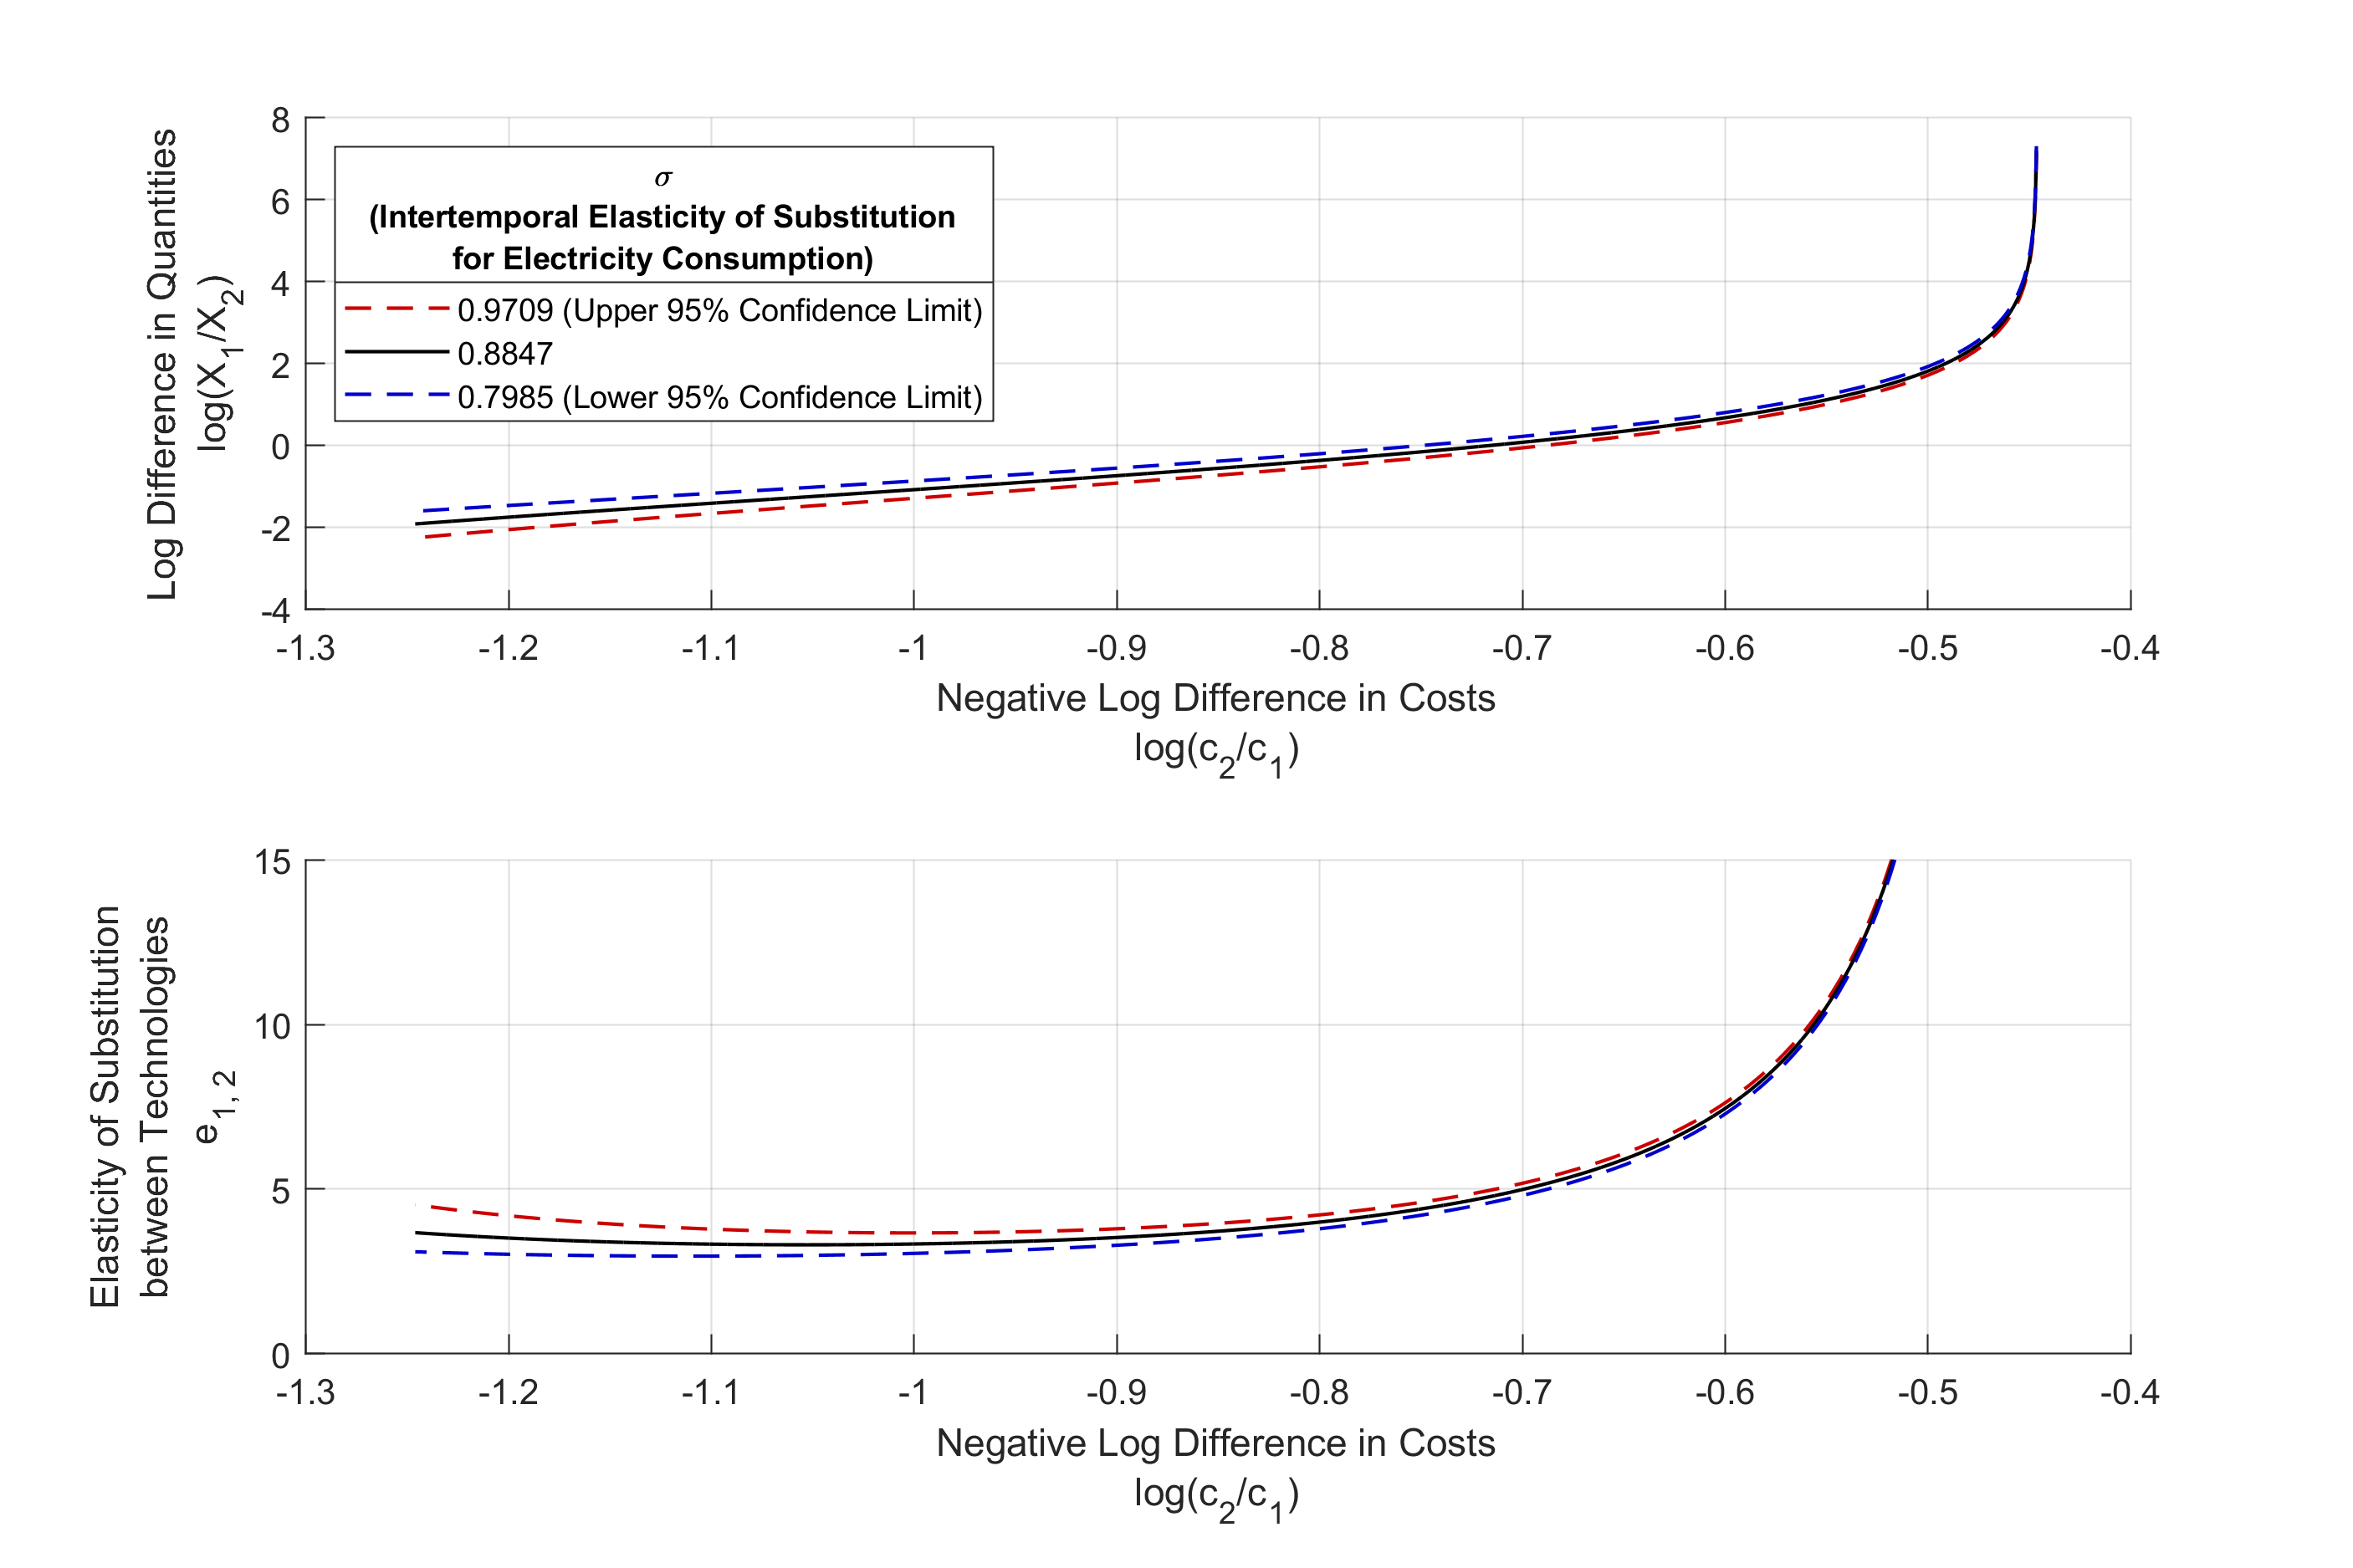
\includegraphics[width=1\linewidth]{../figures/fig_elasticity} \\
			\multicolumn{1}{@{\hspace{0.2in}}p{5.9in}@{}}{ \textit{Note: } Technology 1 is coal and technology 2 is solar. The legend in the upper subplot also applies to the lower subplot. These results were obtained using the following parameters: $\alpha_t = 0.6$, $\alpha_s = 0.4$, $\xi_1 = (1, \, 1)$, $\xi_2 = (1, \, 0.1)$, $c_1 = 104.3$, $c_2 = 60$. Furthermore, we set the parameter for the intertemporal elasticity of substitution for electricity consumption equal to our estimate $\hat{\sigma} = 0.8847$. In order to generate these numerical results, we first found the optimal quantities of $\mathbf{X}$ over a range of prices $c_1^* \in (0.5\, c_1, 2 \,c_1)$. Then, we obtained estimates of the elasticity of substitution by numerically differentiating $\ln(X_1/X_2)$ with respect to $-\ln(c_1/ c_2)$. That is, the elasticity of substitution  between technology 1 and 2 is given by the slope of the upper subplot, and it is graphed in the lower subplot. Finally, we repeat this procedure with $\sigma$ equal to two standard deviations above and below its estimated value $\hat{\sigma}$; that is, the dashed lines represent  $\sigma = 0.8847 \pm (1.96)(0.044)$. }     \\  
		\end{tabular}
	\end{figure}
	\clearpage
	
	\begin{figure}[!h]
		\caption{The Price Elasticity of Demand for Coal Power} 
		\label{fig:coalelas}
		\footnotesize
		\vspace{-1em}
		\begin{tabular}{@{\extracolsep{0em}}c}
			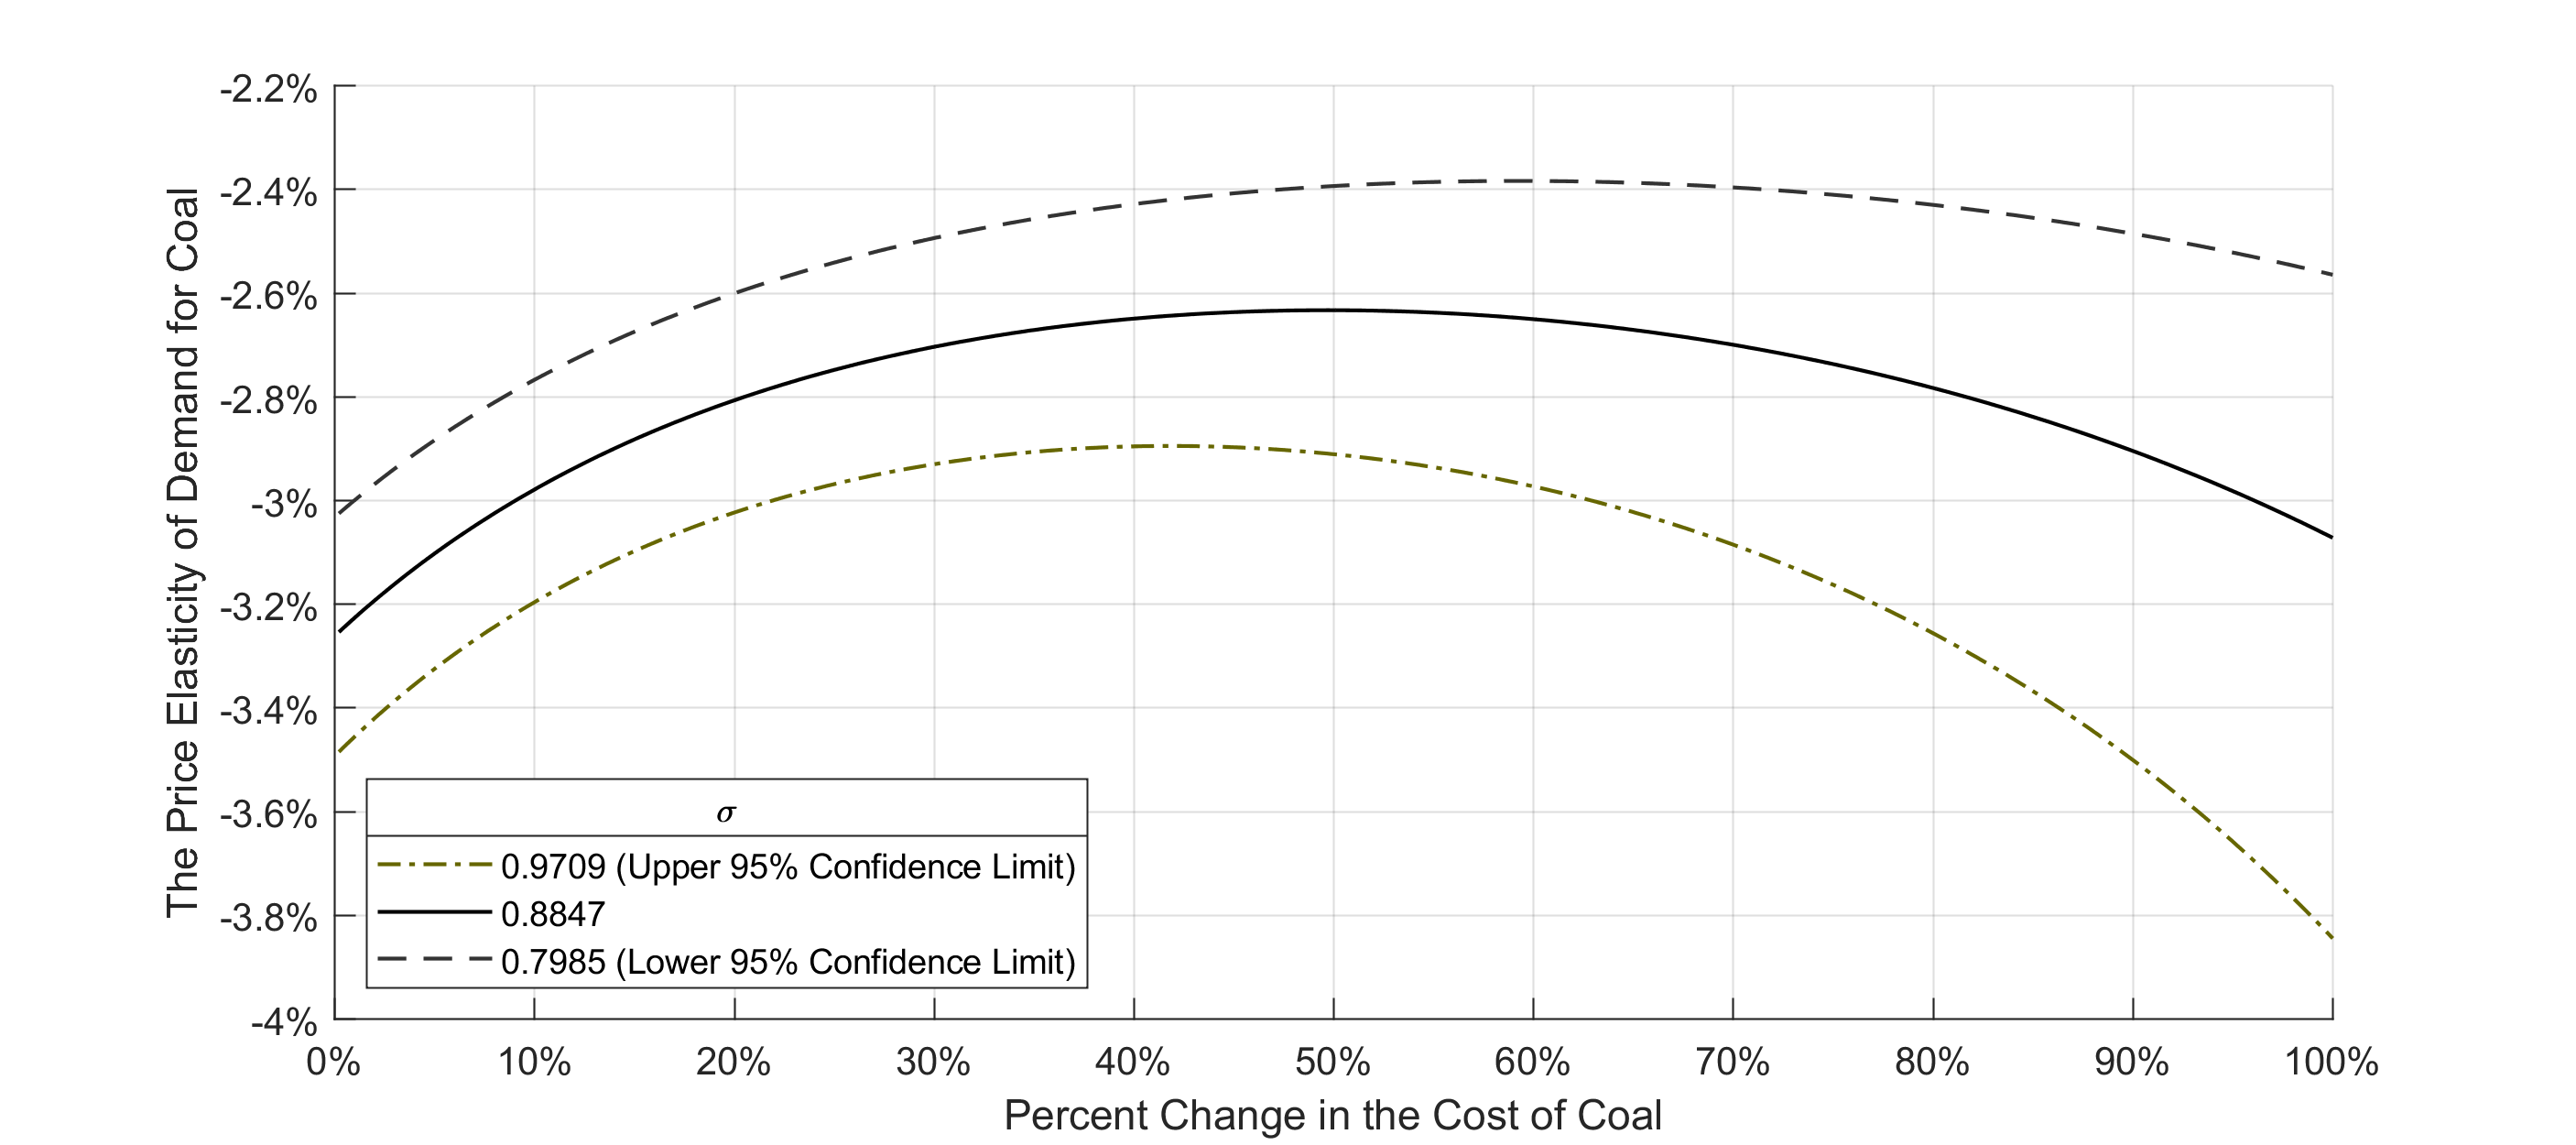
\includegraphics[width=1\linewidth]{../figures/fig_coal_elas} \\
			\multicolumn{1}{@{\hspace{0.2in}}p{5.9in}@{}}{ \textit{Note: } These results were obtained using the following parameters: $\alpha_t = 0.6$, $\alpha_s = 0.4$, $\xi_1 = (1, \, 1)$, $\xi_2 = (1, \, 0.1)$, $c_1 = 104.3$, $c_2 = 60$, $\sigma = 0.5$. We generate these results by finding the optimal quantity of coal, $X_1$, over a range of percent changes in its price $c_1$. Then, on the y-axis, we plot the log difference in $X_1$ divided by the log difference in its price. This is equivalent to the price elasticity of demand for $X_1$. }     \\  
		\end{tabular}
	\end{figure}
	\clearpage
	
	\begin{figure}[!h]
		\captionsetup{format=centerproper}
		\caption{The Effect of Battery Storage on the Elasticity\newline of Substitution between Solar and Coal} 
		\label{fig:battery}
		\footnotesize
		\vspace{-1em}
		\begin{tabular}{@{\extracolsep{0em}}c}
			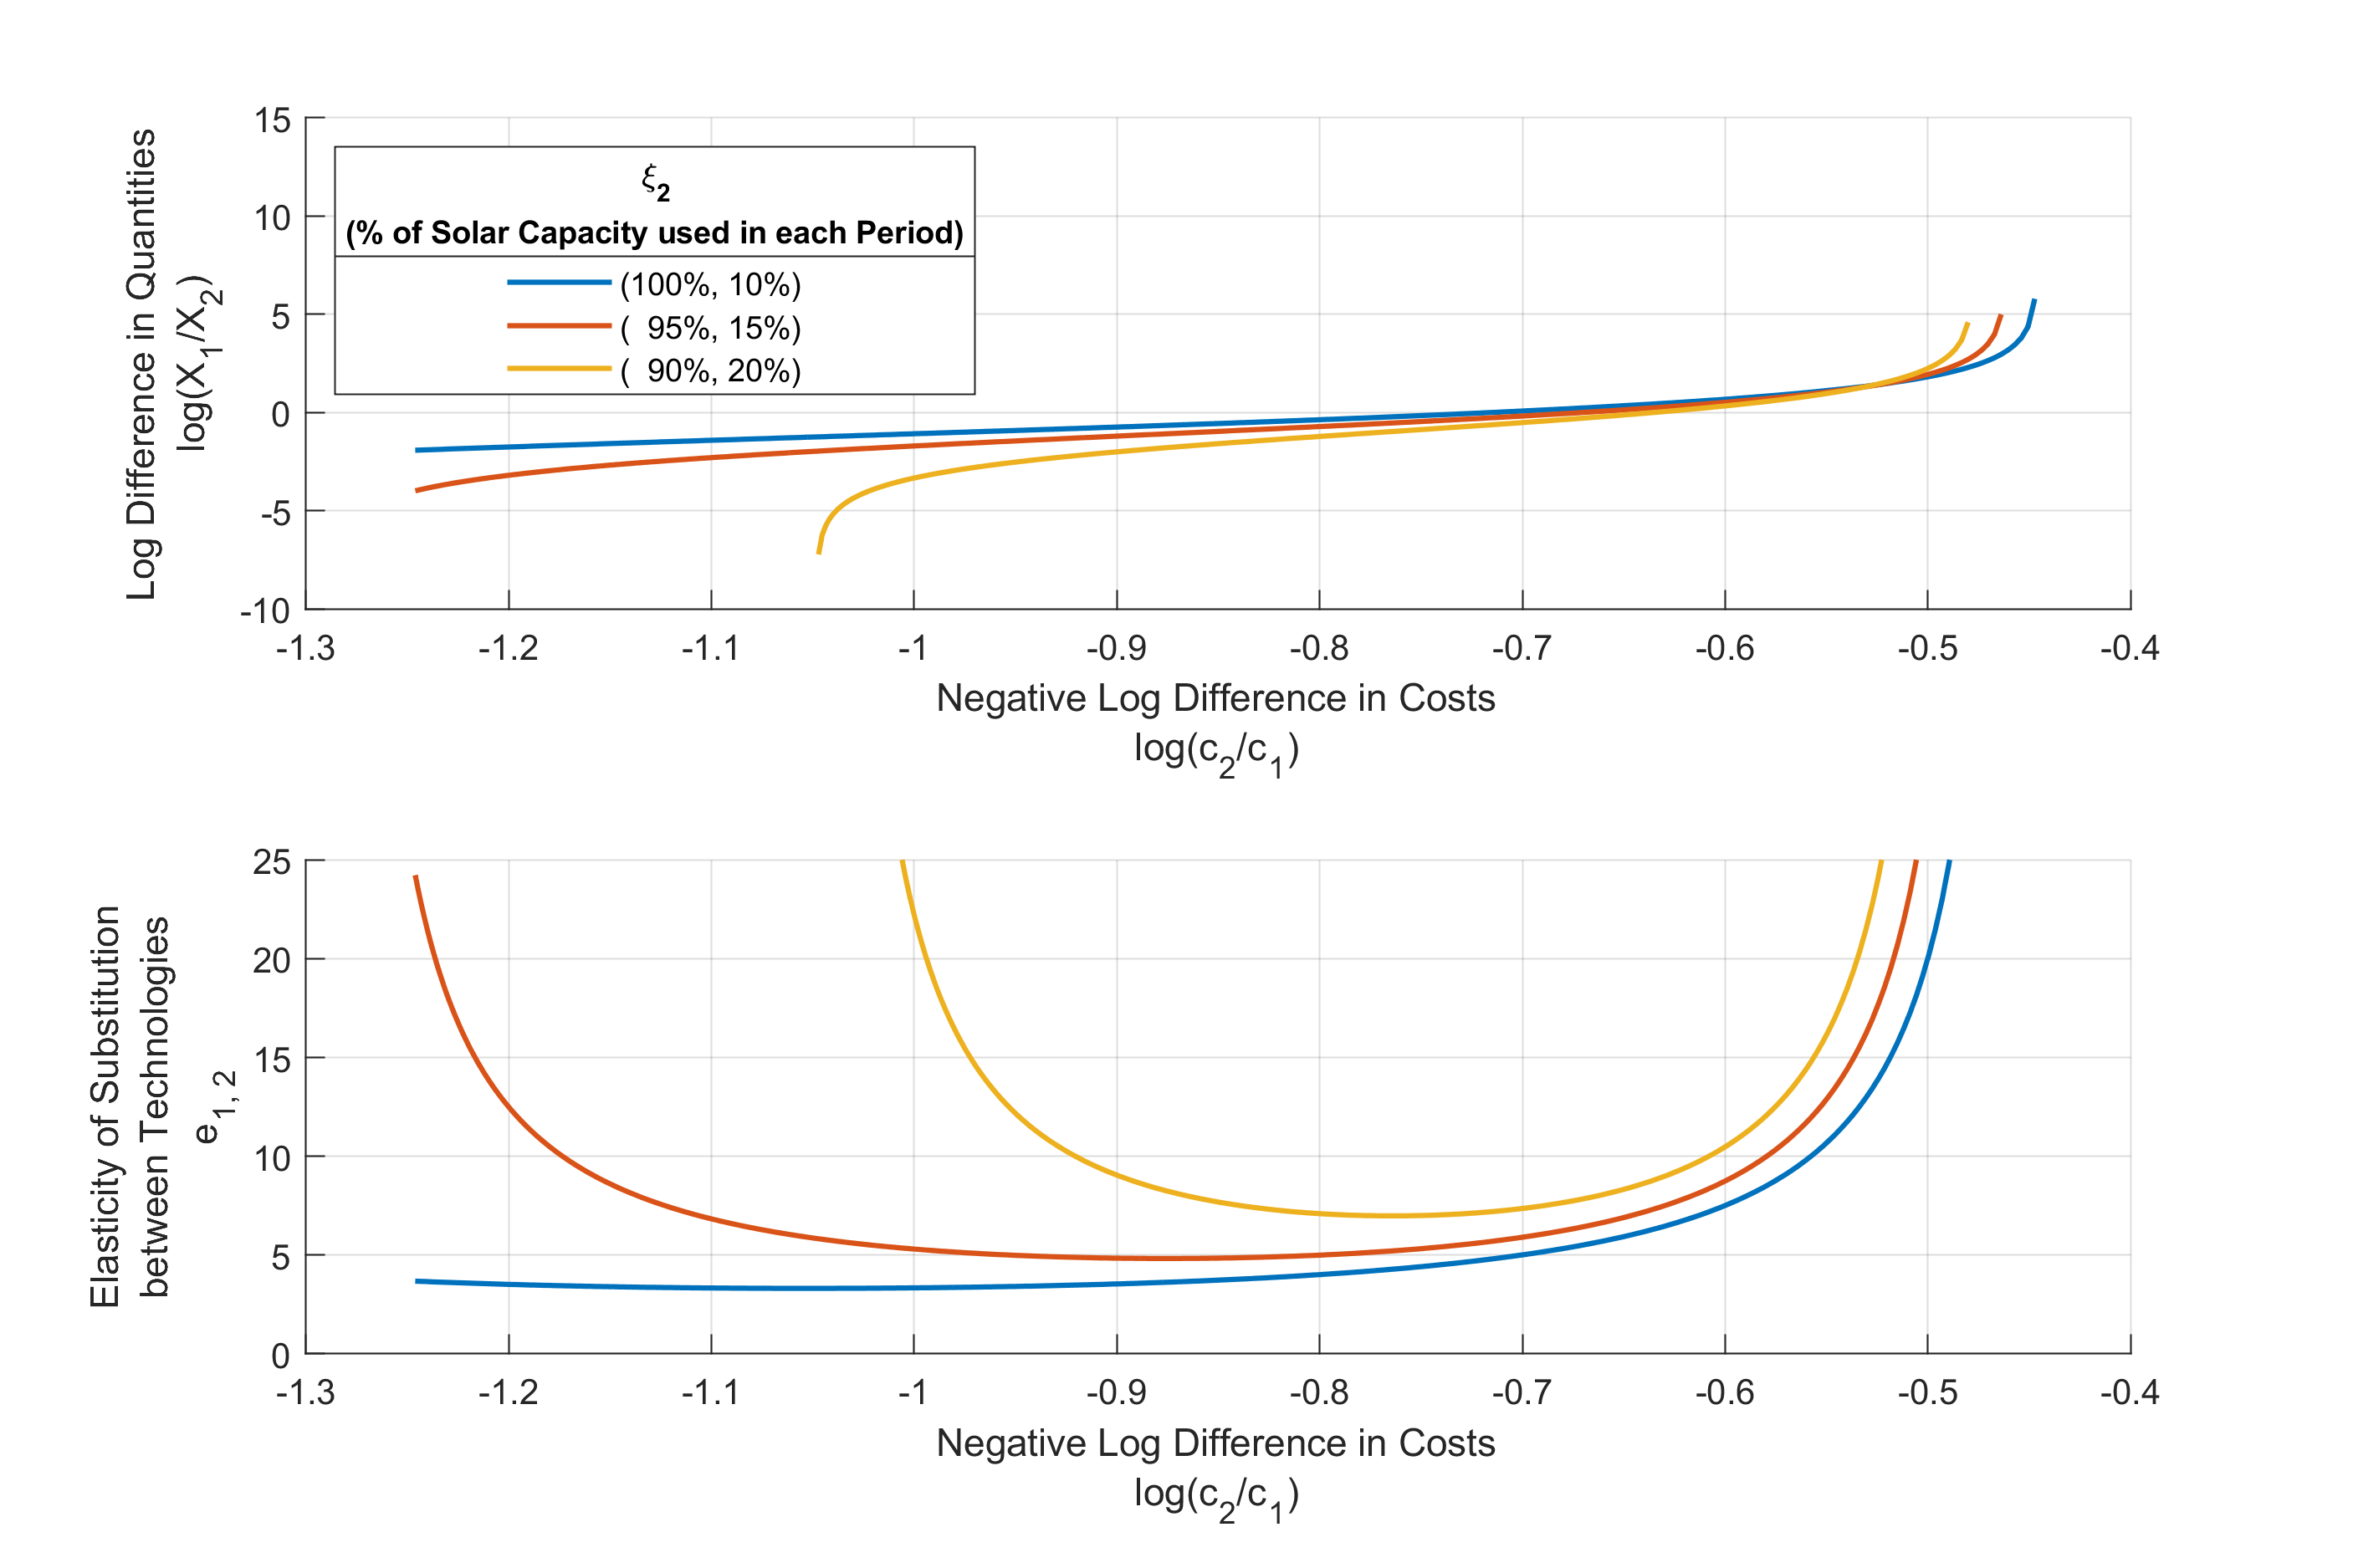
\includegraphics[width=1\linewidth]{../figures/fig_batteries} \\
			\multicolumn{1}{@{\hspace{0.2in}}p{5.9in}@{}}{ \textit{Note: } Technology 1 is coal and technology 2 is solar. The legend in the upper subplot also applies to the lower subplot. The elasticity of substitution  between technology 1 and 2 is given by the slope of the upper subplot, and it is graphed in the lower subplot.  These results were obtained using the following parameters: $\alpha_t = 0.6$, $\alpha_s = 0.4$, $\xi_1 = (1, \, 1)$, $\xi_2 = (1, \, 0.1)$, $c_1 = 104.3$, $c_2 = 60$. Furthermore, we set the parameter for the intertemporal elasticity of substitution for electricity consumption equal to our estimate $\hat{\sigma} = 0.8847$. We generated these numerical results with the same procedure used for \autoref{fig:eosnum}. We repeated this procedure with $\xi_2 = (0.95, 0.15)$ and $\xi_2 = (0.90, 0.20)$ to simulate the effects of shifting solar power output using batteries. }     \\  
		\end{tabular}
	\end{figure}
	\clearpage
	
	\begin{table}[!h] \centering 
		\captionsetup{format=centerproper}
		\caption{The Effect of Battery Storage on the   \newline Elasticity of Demand for Coal Power} 
		\label{table:storelas} 
		\small
		\begin{tabular}{@{\extracolsep{2em}}ccc} 
			\\[-4ex]\hline  
			\hline \\[-1.8ex] 
			\\[-2.6ex] \specialcell{Solar Output during \\ Peak Hours ($\xi_{2t}$)} &  \specialcell{Solar Output during \\ Off-Peak Hours ($\xi_{2s}$)}  & \specialcell{The Elasticity of  \\ Demand for Coal Power}\\ [0.5ex]
			\hline \\[-1.8ex] 
			100\% &  \phantom{1}5\%  &  -3.25 \\
			\phantom{1}95\% &            10\%  &  -3.71 \\
			\phantom{1}90\% &            15\%  &  -4.40 \\
			\phantom{1}85\% &            20\%  &  -5.48 \\
			\phantom{1}80\% &            25\%  &  -7.29 \\
			\hline 
			\hline \\[-1.8ex] 
			\multicolumn{3}{@{}p{34.2em}@{}}{\textit{Note: } These results were obtained using the following parameters: $\alpha_t = 0.6$, $\alpha_s = 0.4$, $\xi_1 = (1, \, 1)$, $c_1 = 104.3$, $c_2 = 60$, $\sigma = 0.8847$. We generated these results by numerically differentiating the optimal quantity of coal power, $X_1$, with respect to its own price, $c_1$, around its initial price $104.3$. We repeated this process for various values of the output parameter for solar power, $\xi_{2}$. Specifically, we considered 5\% to 20\% shifts in the output of solar power from peak to  off-peak hours to simulate the effects of implementing battery storage. }  \\ 
		\end{tabular} 
	\end{table} 
	\clearpage
	
	\begin{figure}[!h]
		\captionsetup{format=centerproper}
		\caption{The VES Approximation of the Elasticity of Substitution \\ between Solar and Coal } 
		\label{fig:ves}
		\footnotesize
		\vspace{-1em}
		\begin{tabular}{@{\extracolsep{0em}}c}
			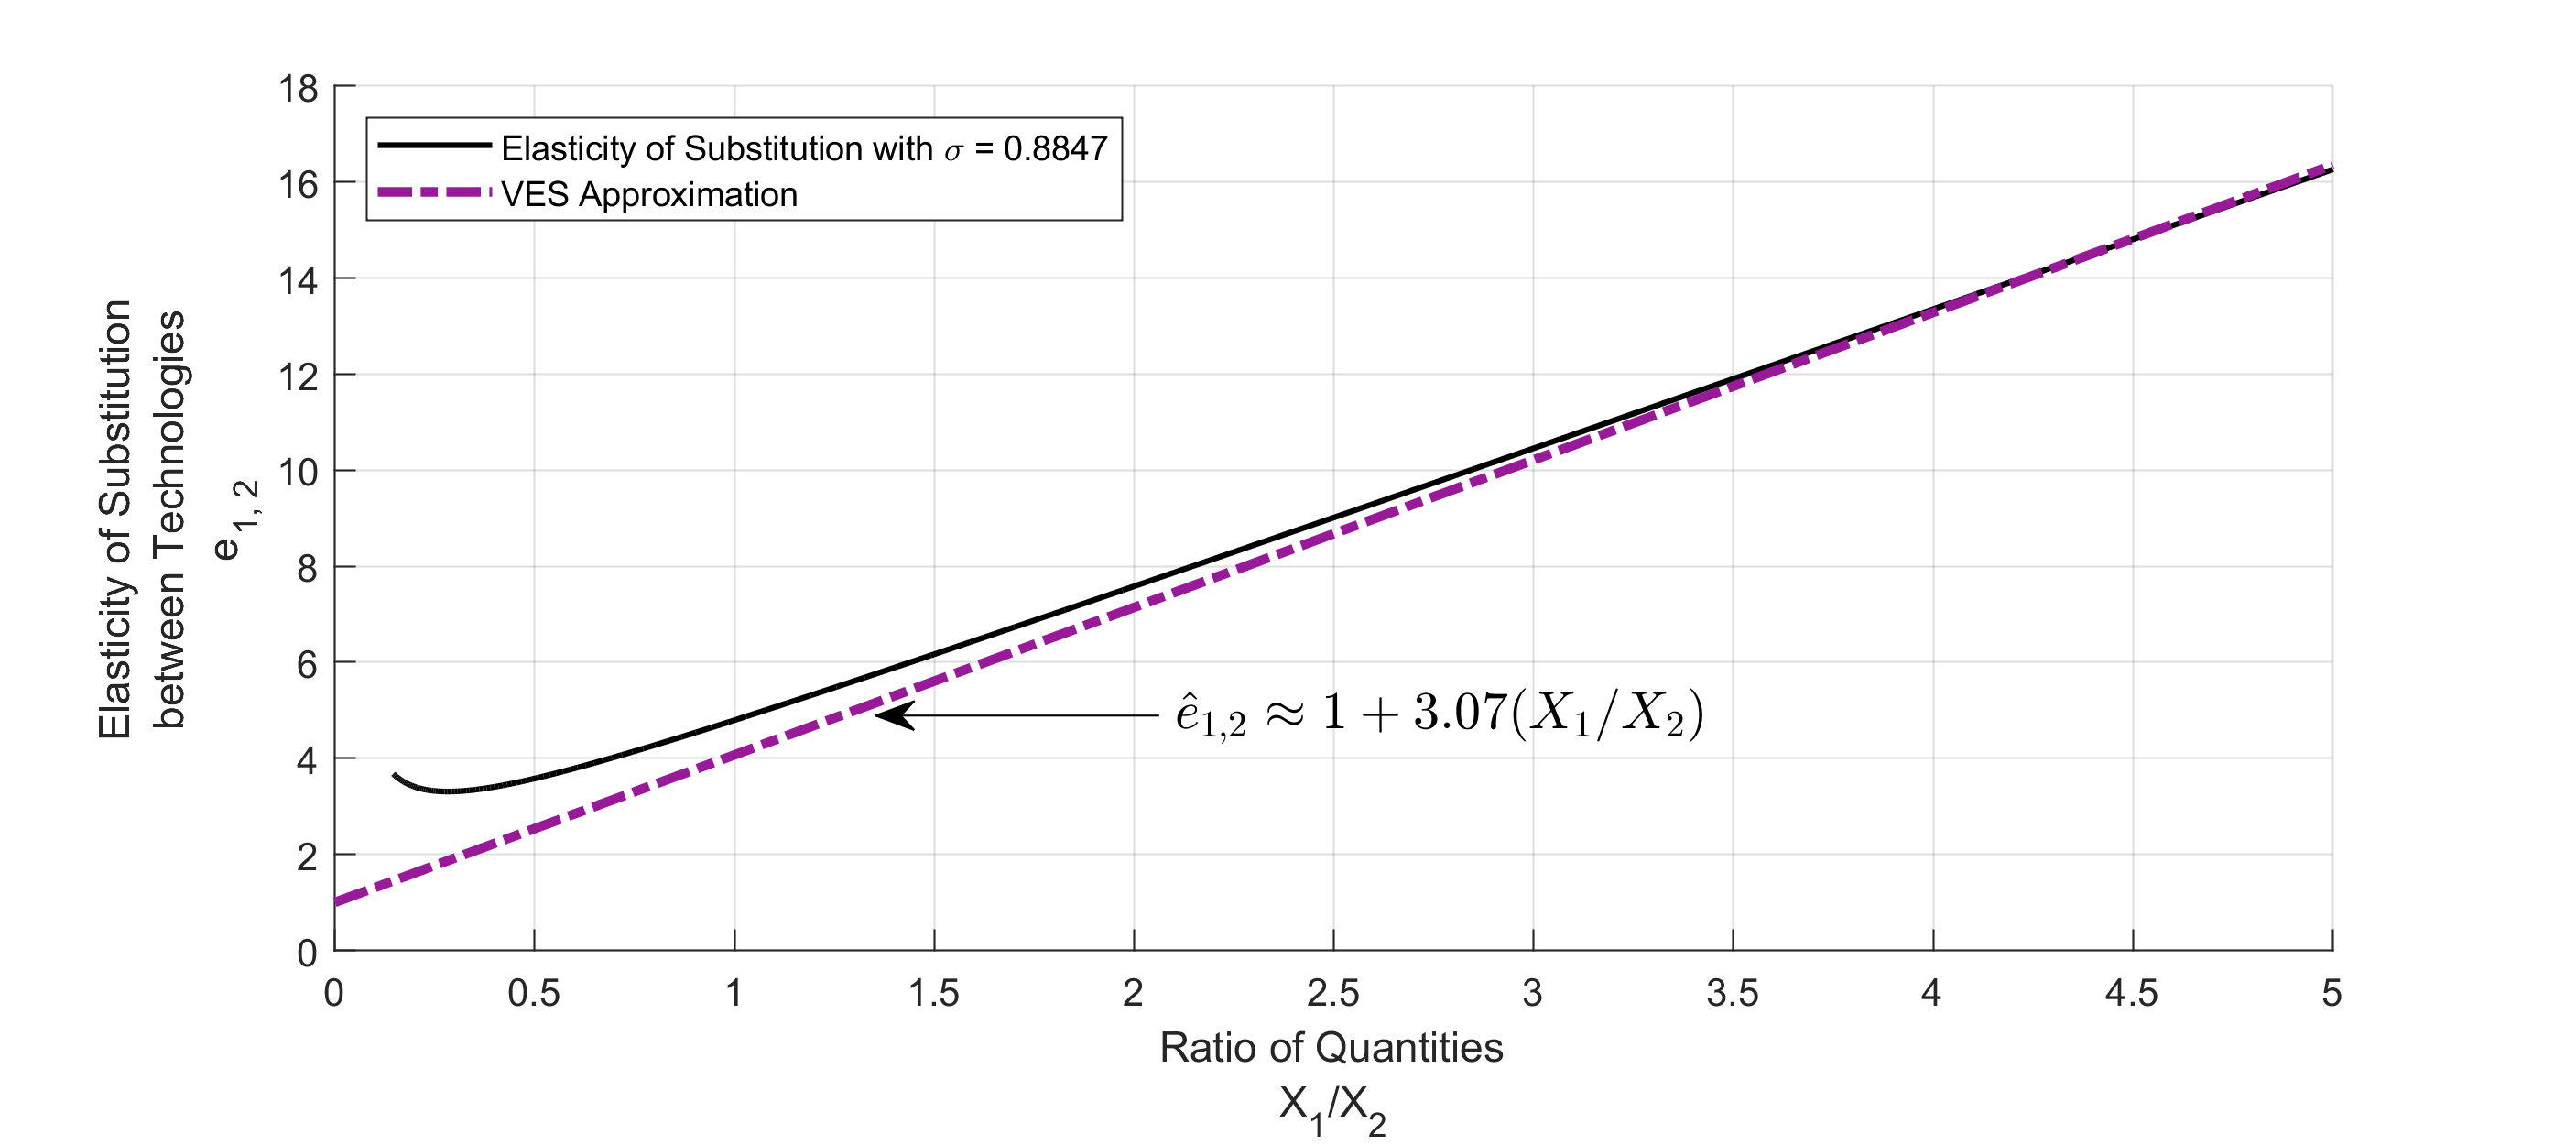
\includegraphics[width=1\linewidth]{../figures/fig_ves_approx} \\
			\multicolumn{1}{@{\hspace{0.2in}}p{5.9in}@{}}{ \textit{Note: } Technology 1 is coal and technology 2 is solar. The purple, dash-dots line represents a linear approximation of $e_{1,2}$ for $\sigma = 0.8847$ with a fixed intercept of 1. These results were obtained using the following parameters: $\alpha_t = 0.6$, $\alpha_s = 0.4$, $\xi_1 = (1, \, 1)$, $\xi_2 = (1, \, 0.1)$, $c_1 = 104.3$, $c_2 = 60$. Furthermore, we set the parameter for the intertemporal elasticity of substitution for electricity consumption equal to our estimate $\hat{\sigma} = 0.8847$. In order to generate these numerical results, we first found the optimal quantities of $\mathbf{X}$ over a range of prices $c_1^* \in (0.5\, c_1, 2 \,c_1)$. Then, we obtained estimates of the elasticity of substitution by numerically differentiating $\ln(X_1/X_2)$ with respect to $-\ln(c_1, c_2)$.  }     \\  
		\end{tabular}
	\end{figure}
	\clearpage
	
		
	
	\begin{table}[h!]
		\caption{Parameter Restrictions for $Z, X > 0$} 
		\label{tab:paramrest}
		\small
		\centering
		\begin{tabular}{@{\extracolsep{2em}}l@{\hspace{-0.5 em}}cc}
			\\[-4ex]
			\toprule \\[-2.5ex]
			& \textbf{Case 1} & \textbf{Case 2 } \\
			\cmidrule(lr){2-2} \cmidrule(lr){3-3} \\[-1.5ex]
			\textbf{Cost Efficiency}& $\xi_{2t}/c_2 > \xi_{1t}/c_1$ & $\xi_{2t}/c_2 < \xi_{1t}/c_1 $\\
			\textbf{Restrictions} & $\xi_{1s}/c_1 > \xi_{2s}/c_2$  & $\xi_{1s}/c_1 < \xi_{2s}/c_2 $ 		\\ [3ex]
			\textbf{Output Efficiency}& $\xi_{2t}/\xi_{2s} > \xi_{1t}/\xi_{1s}$ & $\xi_{2t}/\xi_{2s} < \xi_{1t}/\xi_{1s}$\\
			\textbf{Restrictions} & $\xi_{1s}/\xi_{1t} > \xi_{2s}/\xi_{2t} $  & $\xi_{1s}/\xi_{1t} < \xi_{2s}/\xi_{2t}  $ 		\\ [3ex]
			\multirow{2}{10em}{\textbf{Mixed Efficiency Restrictions}}& $\dfrac{\alpha_s \left(\xi_{1s}/c_1 - \xi_{2s}/c_2\right)}{\alpha_t \left( \xi_{2t}/c_2 - \xi_{1t}/c_1 \right)} > \xi_{2s}/\xi_{2t}$ & $\dfrac{\alpha_s \left(\xi_{1s}/c_1 - \xi_{2s}/c_2\right)}{\alpha_t \left( \xi_{2t}/c_2 - \xi_{1t}/c_1 \right)} < \xi_{2s}/\xi_{2t}$\\
			& $\dfrac{\alpha_s \left(\xi_{1s}/c_1 - \xi_{2s}/c_2\right)}{\alpha_t \left( \xi_{2t}/c_2 - \xi_{1t}/c_1 \right)} < \xi_{1s}/\xi_{1t} $  & $\dfrac{\alpha_s \left(\xi_{1s}/c_1 - \xi_{2s}/c_2\right)}{\alpha_t \left( \xi_{2t}/c_2 - \xi_{1t}/c_1 \right)} > \xi_{1s}/\xi_{1t} $ 		\\[2ex] 
			\midrule
			\multicolumn{3}{@{}p{40em}@{}}{\footnotesize \textit{Note: } The inequalities in this table assume that all elements of $\xi$ are greater than $0$. The full proof given below provides equivalent restrictions for the zero cases.   }  
		\end{tabular} 
	\end{table}
	\clearpage
	
	\begin{figure}[h!]
		\captionsetup{format=centerproper}
		\caption{Partially Linear IV Regression Estimates with State Drop Outs} 
		\label{fig:regstaterobust}
		\footnotesize
		\vspace{-1em}
		\begin{tabular}{@{\extracolsep{0em}}c}
			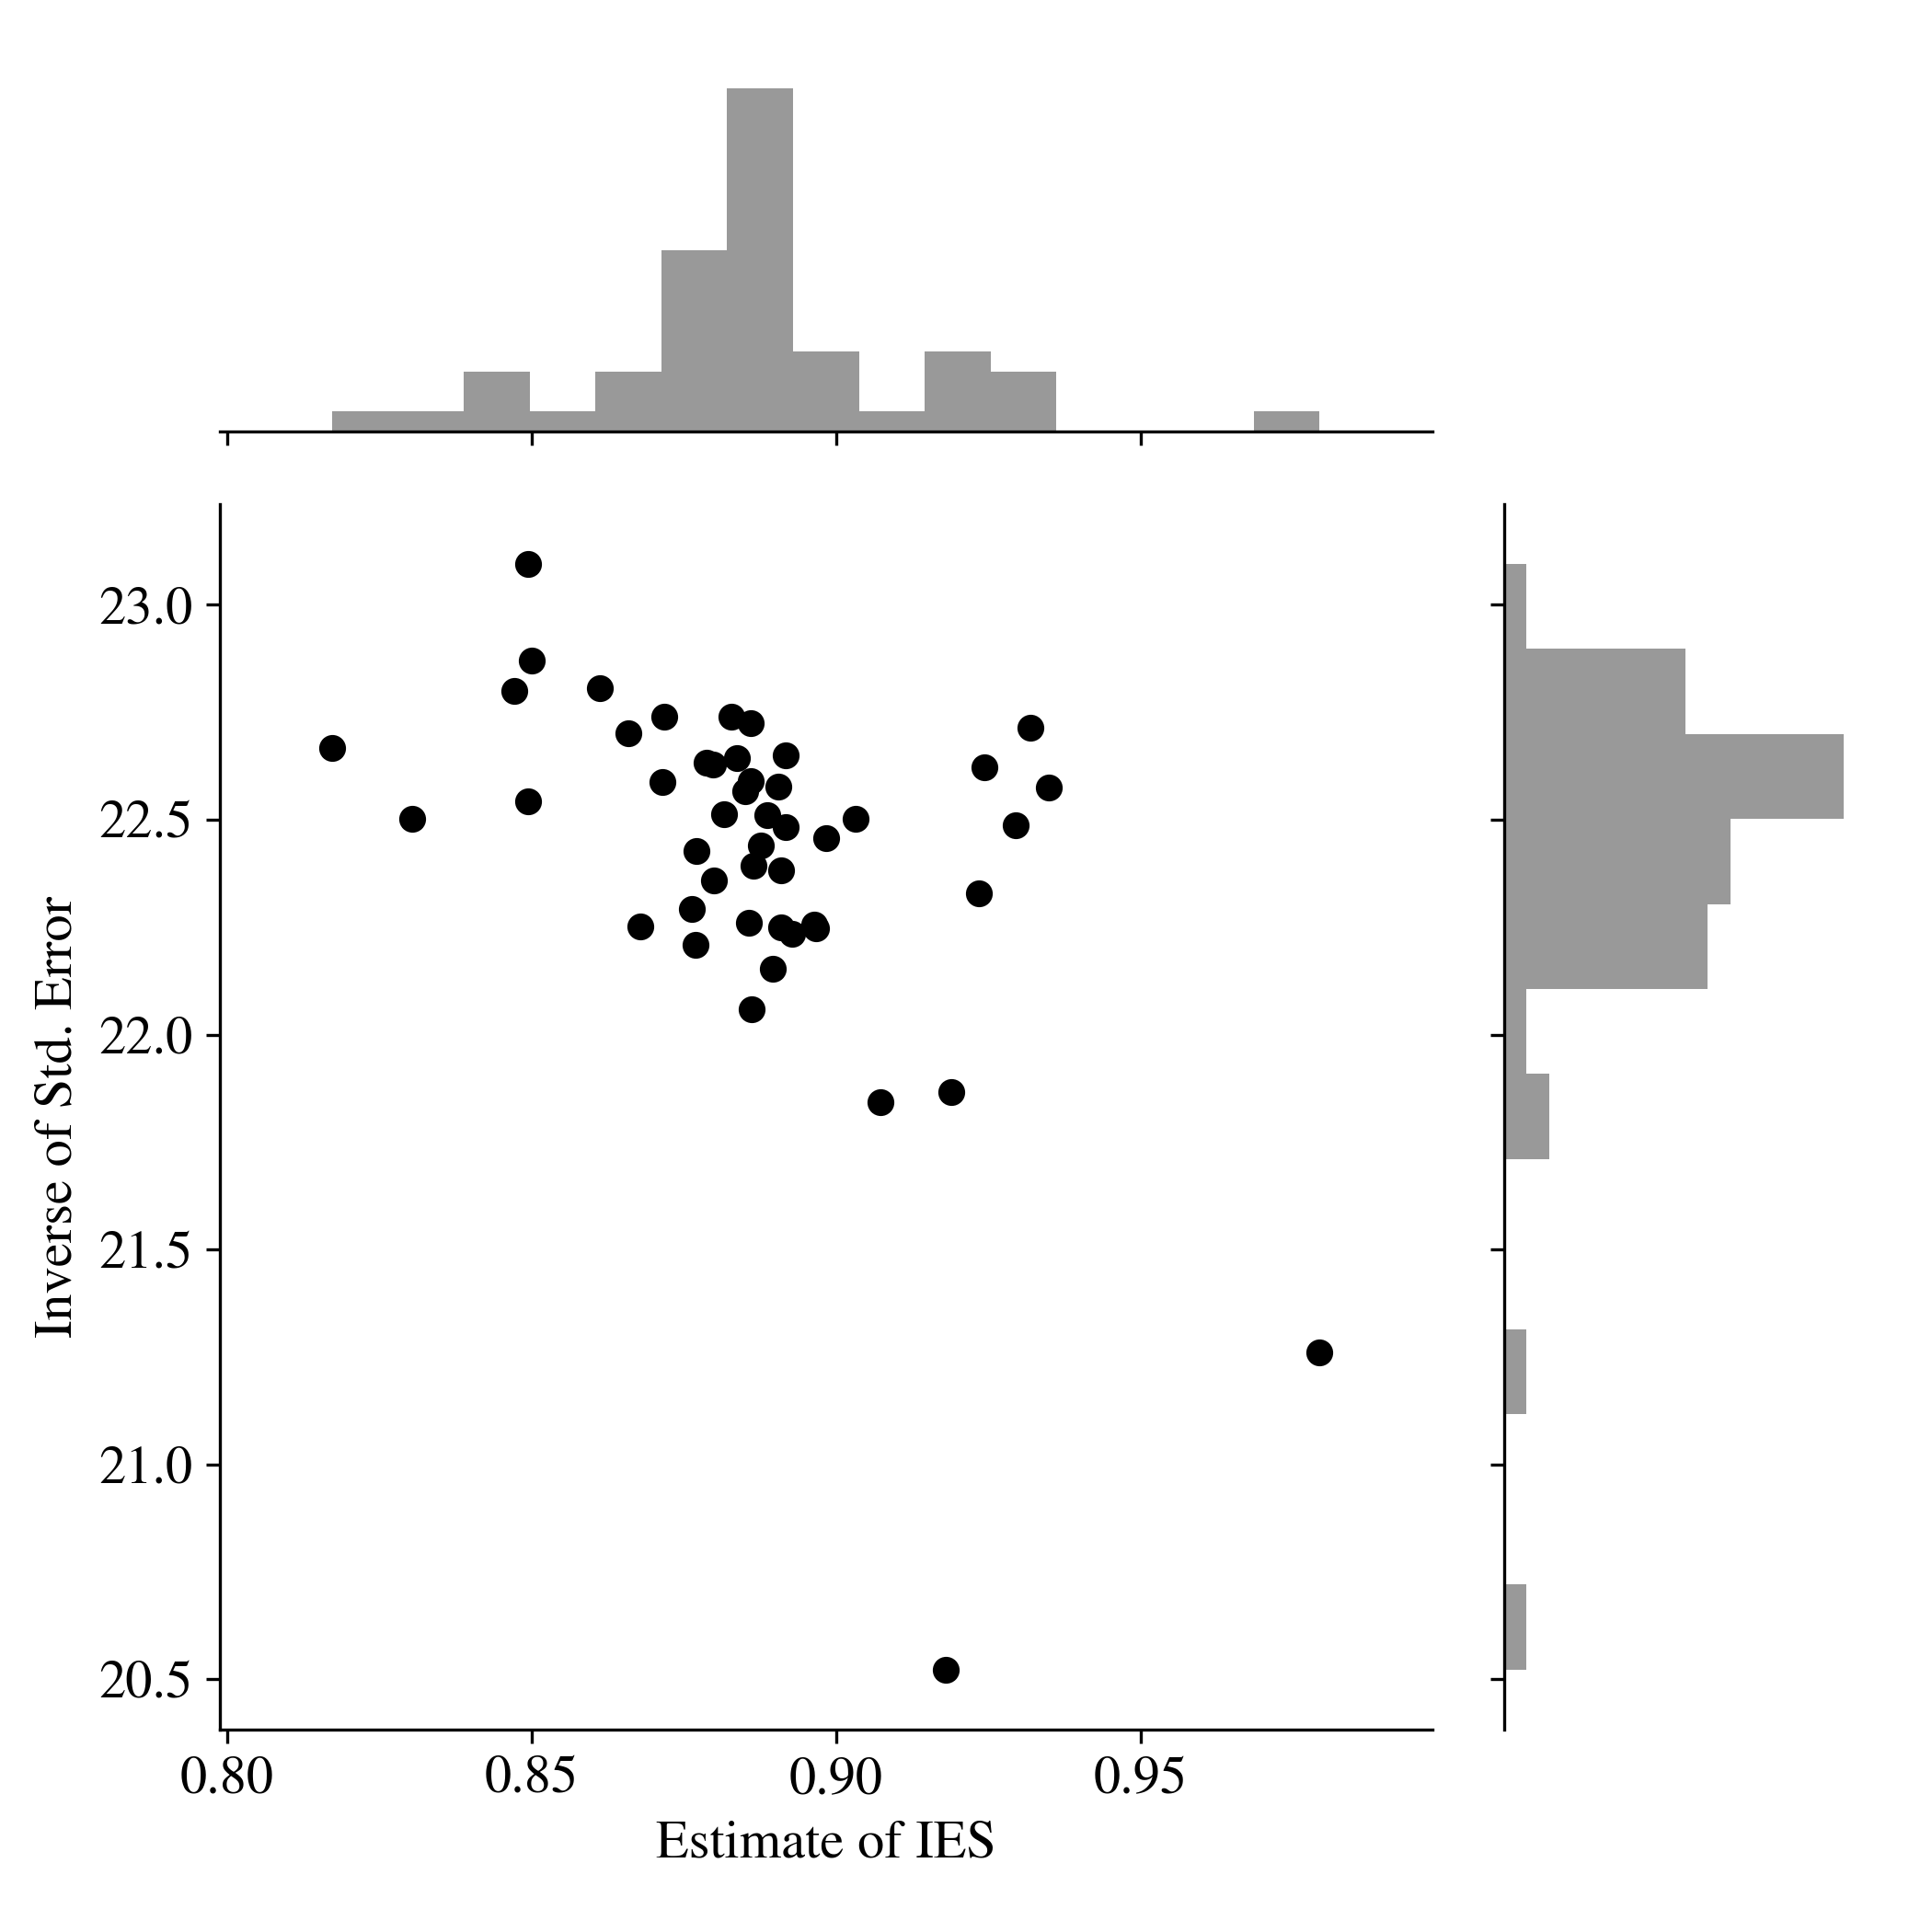
\includegraphics[width=0.75\linewidth]{../figures/regression_state_robustness_check.png} \\
			\multicolumn{1}{@{\hspace{0.2in}}p{5.9in}@{}}{ \textit{Note: } This is a joint plot of the IES  $\hat{\sigma}$ against the inverse of its estimated standard deviation from fit (3) of \autoref{table:pariv}. Each point represents an estimate obtained from regressing on a dataset that drops out one state from the full sample. Since the sample consists of the 48 contiguous US states, this regression is a decrease in sample size of 2.08\% relative to the full dataset. On the top and right side of the graph are histograms for the two variables.}     \\  
		\end{tabular}
	\end{figure}
	\clearpage
	
	\begin{figure}[h!]
		\captionsetup{format=centerproper}
		\caption{The Elasticity of Substitution Between between Solar and Coal \newline  (Robustness Check) } 
		\label{fig:eosrobust}
		\footnotesize
		\vspace{-1em}
		\begin{tabular}{@{\extracolsep{0em}}c}
			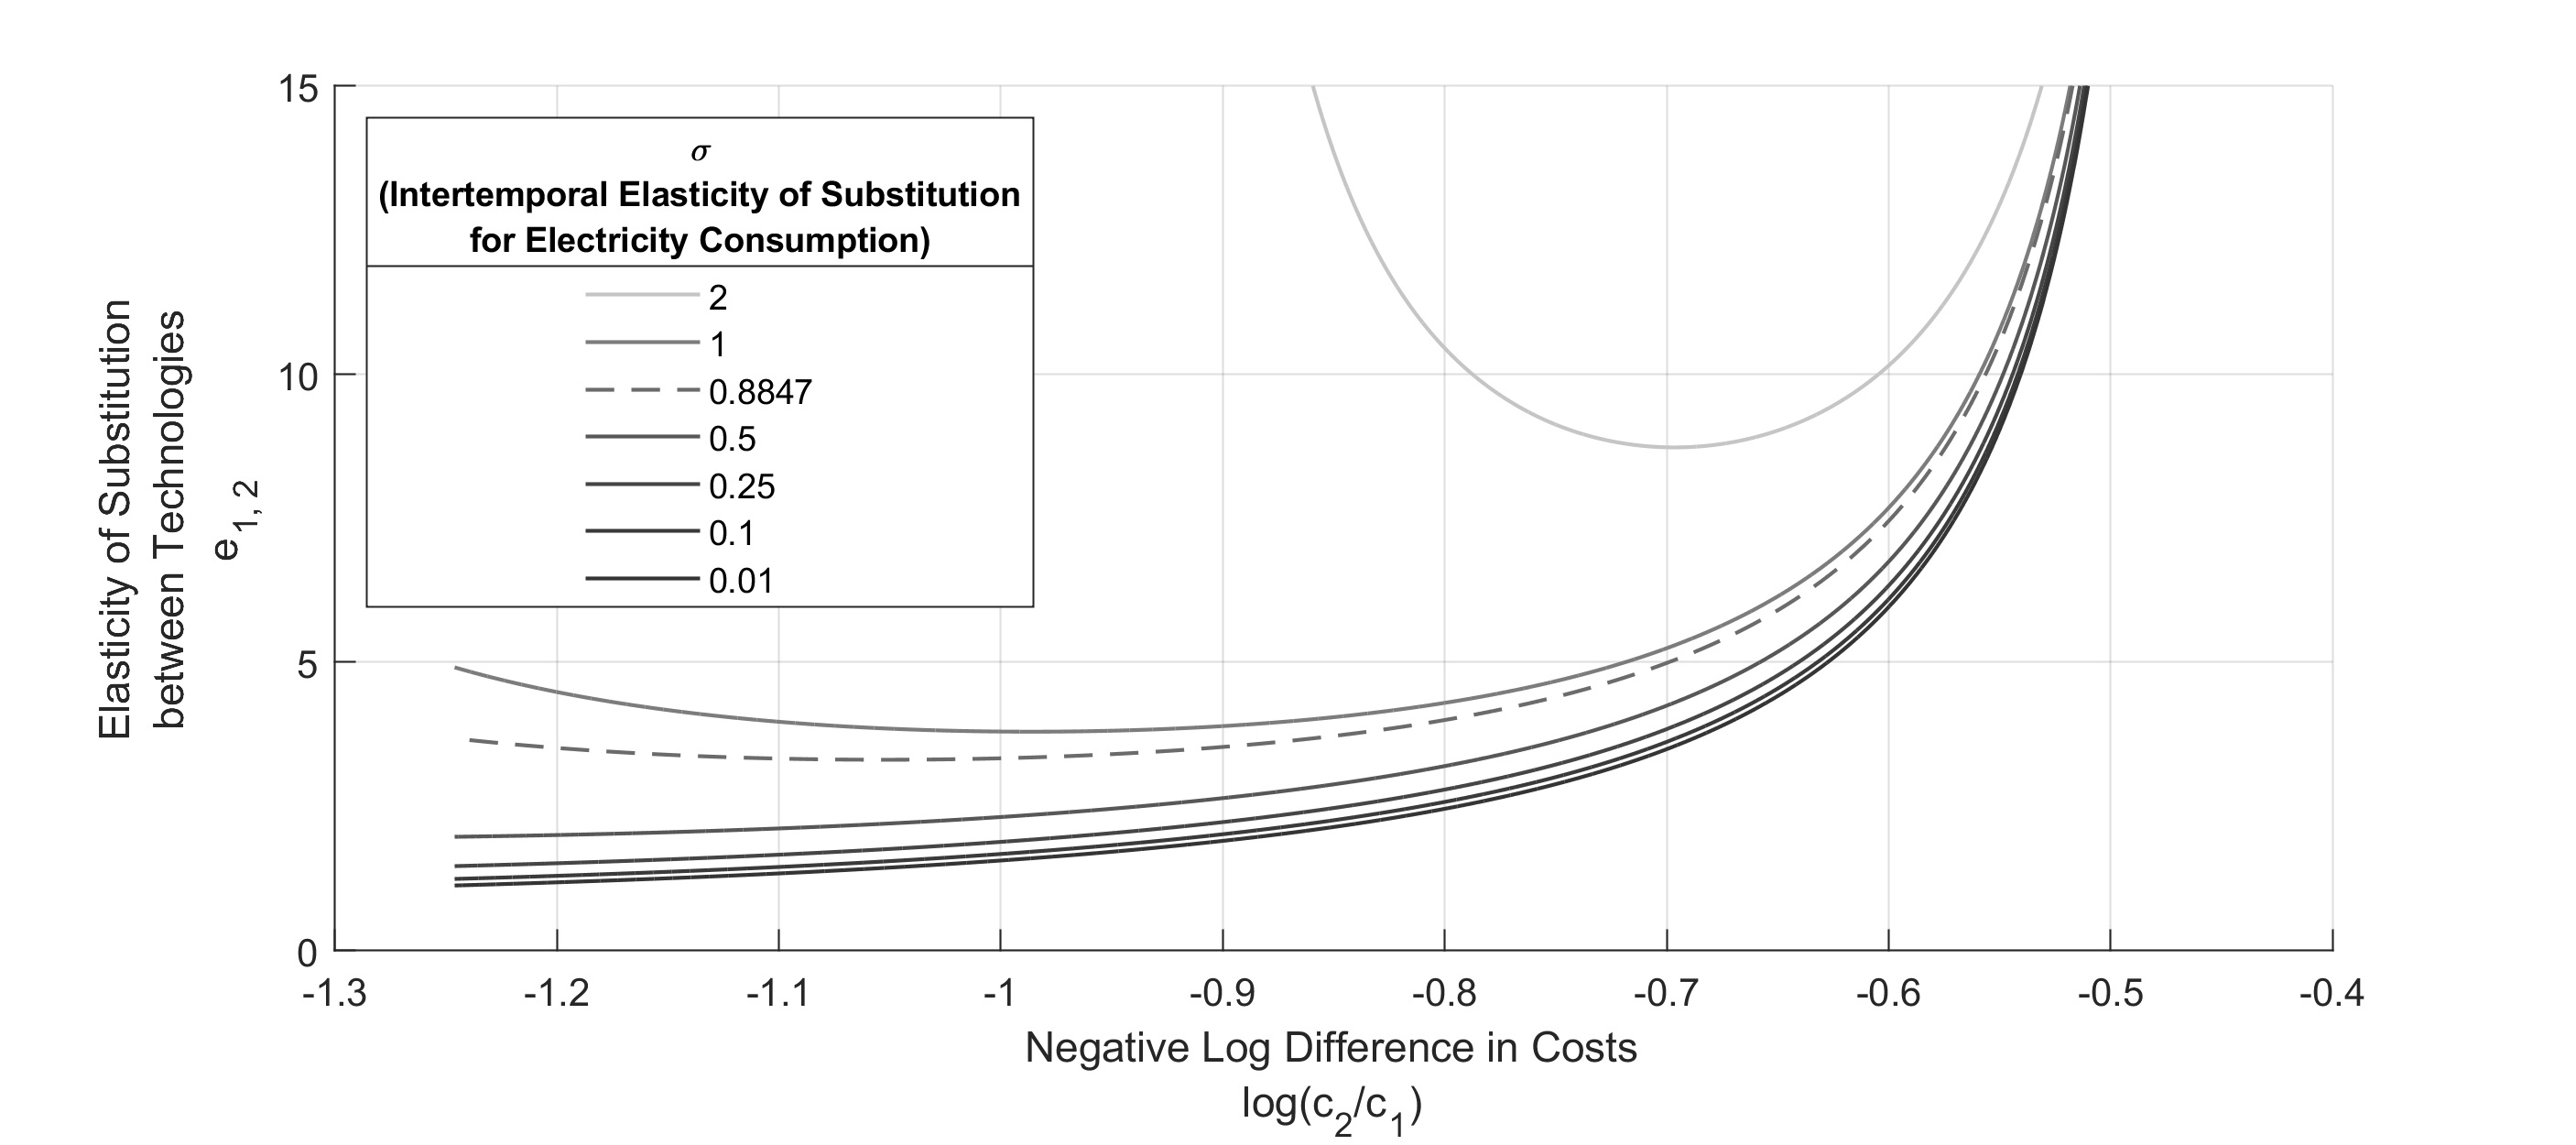
\includegraphics[width=1\linewidth]{../figures/fig_elasticity_robust} \\
			\multicolumn{1}{@{\hspace{0.2in}}p{5.9in}@{}}{ \textit{Note: } This figure is identical to \autoref{fig:eosnum}, but it considers a large range of values for $\sigma$. Technology 1 is coal and technology 2 is solar. The purple, dash-dots line represents a linear approximation of $e_{1,2}$ for $\sigma = 0.8847$ with a fixed intercept of 1. These results were obtained using the following parameters: $\alpha_t = 0.6$, $\alpha_s = 0.4$, $\xi_1 = (1, \, 1)$, $\xi_2 = (1, \, 0.1)$, $c_1 = 104.3$, $c_2 = 60$. Furthermore, we set the parameter for the intertemporal elasticity of substitution for electricity consumption equal to our estimate $\hat{\sigma} = 0.8847$. In order to generate these numerical results, we first found the optimal quantities of $\mathbf{X}$ over a range of prices $c_1^* \in (0.5\, c_1, 2 \,c_1)$. Then, we obtained estimates of the elasticity of substitution by numerically differentiating $\ln(X_1/X_2)$ with respect to $-\ln(c_1, c_2)$. }     \\  
		\end{tabular}
	\end{figure}
	\clearpage
	
	\begin{figure}[h!]
		\captionsetup{format=centerproper}
		\caption{The Elasticity of Substitution Between Two \newline  Minimally Intermittent Technologies} 
		\label{fig:eosrange}
		\footnotesize
		\vspace{-1em}
		\begin{tabular}{@{\extracolsep{0em}}c}
			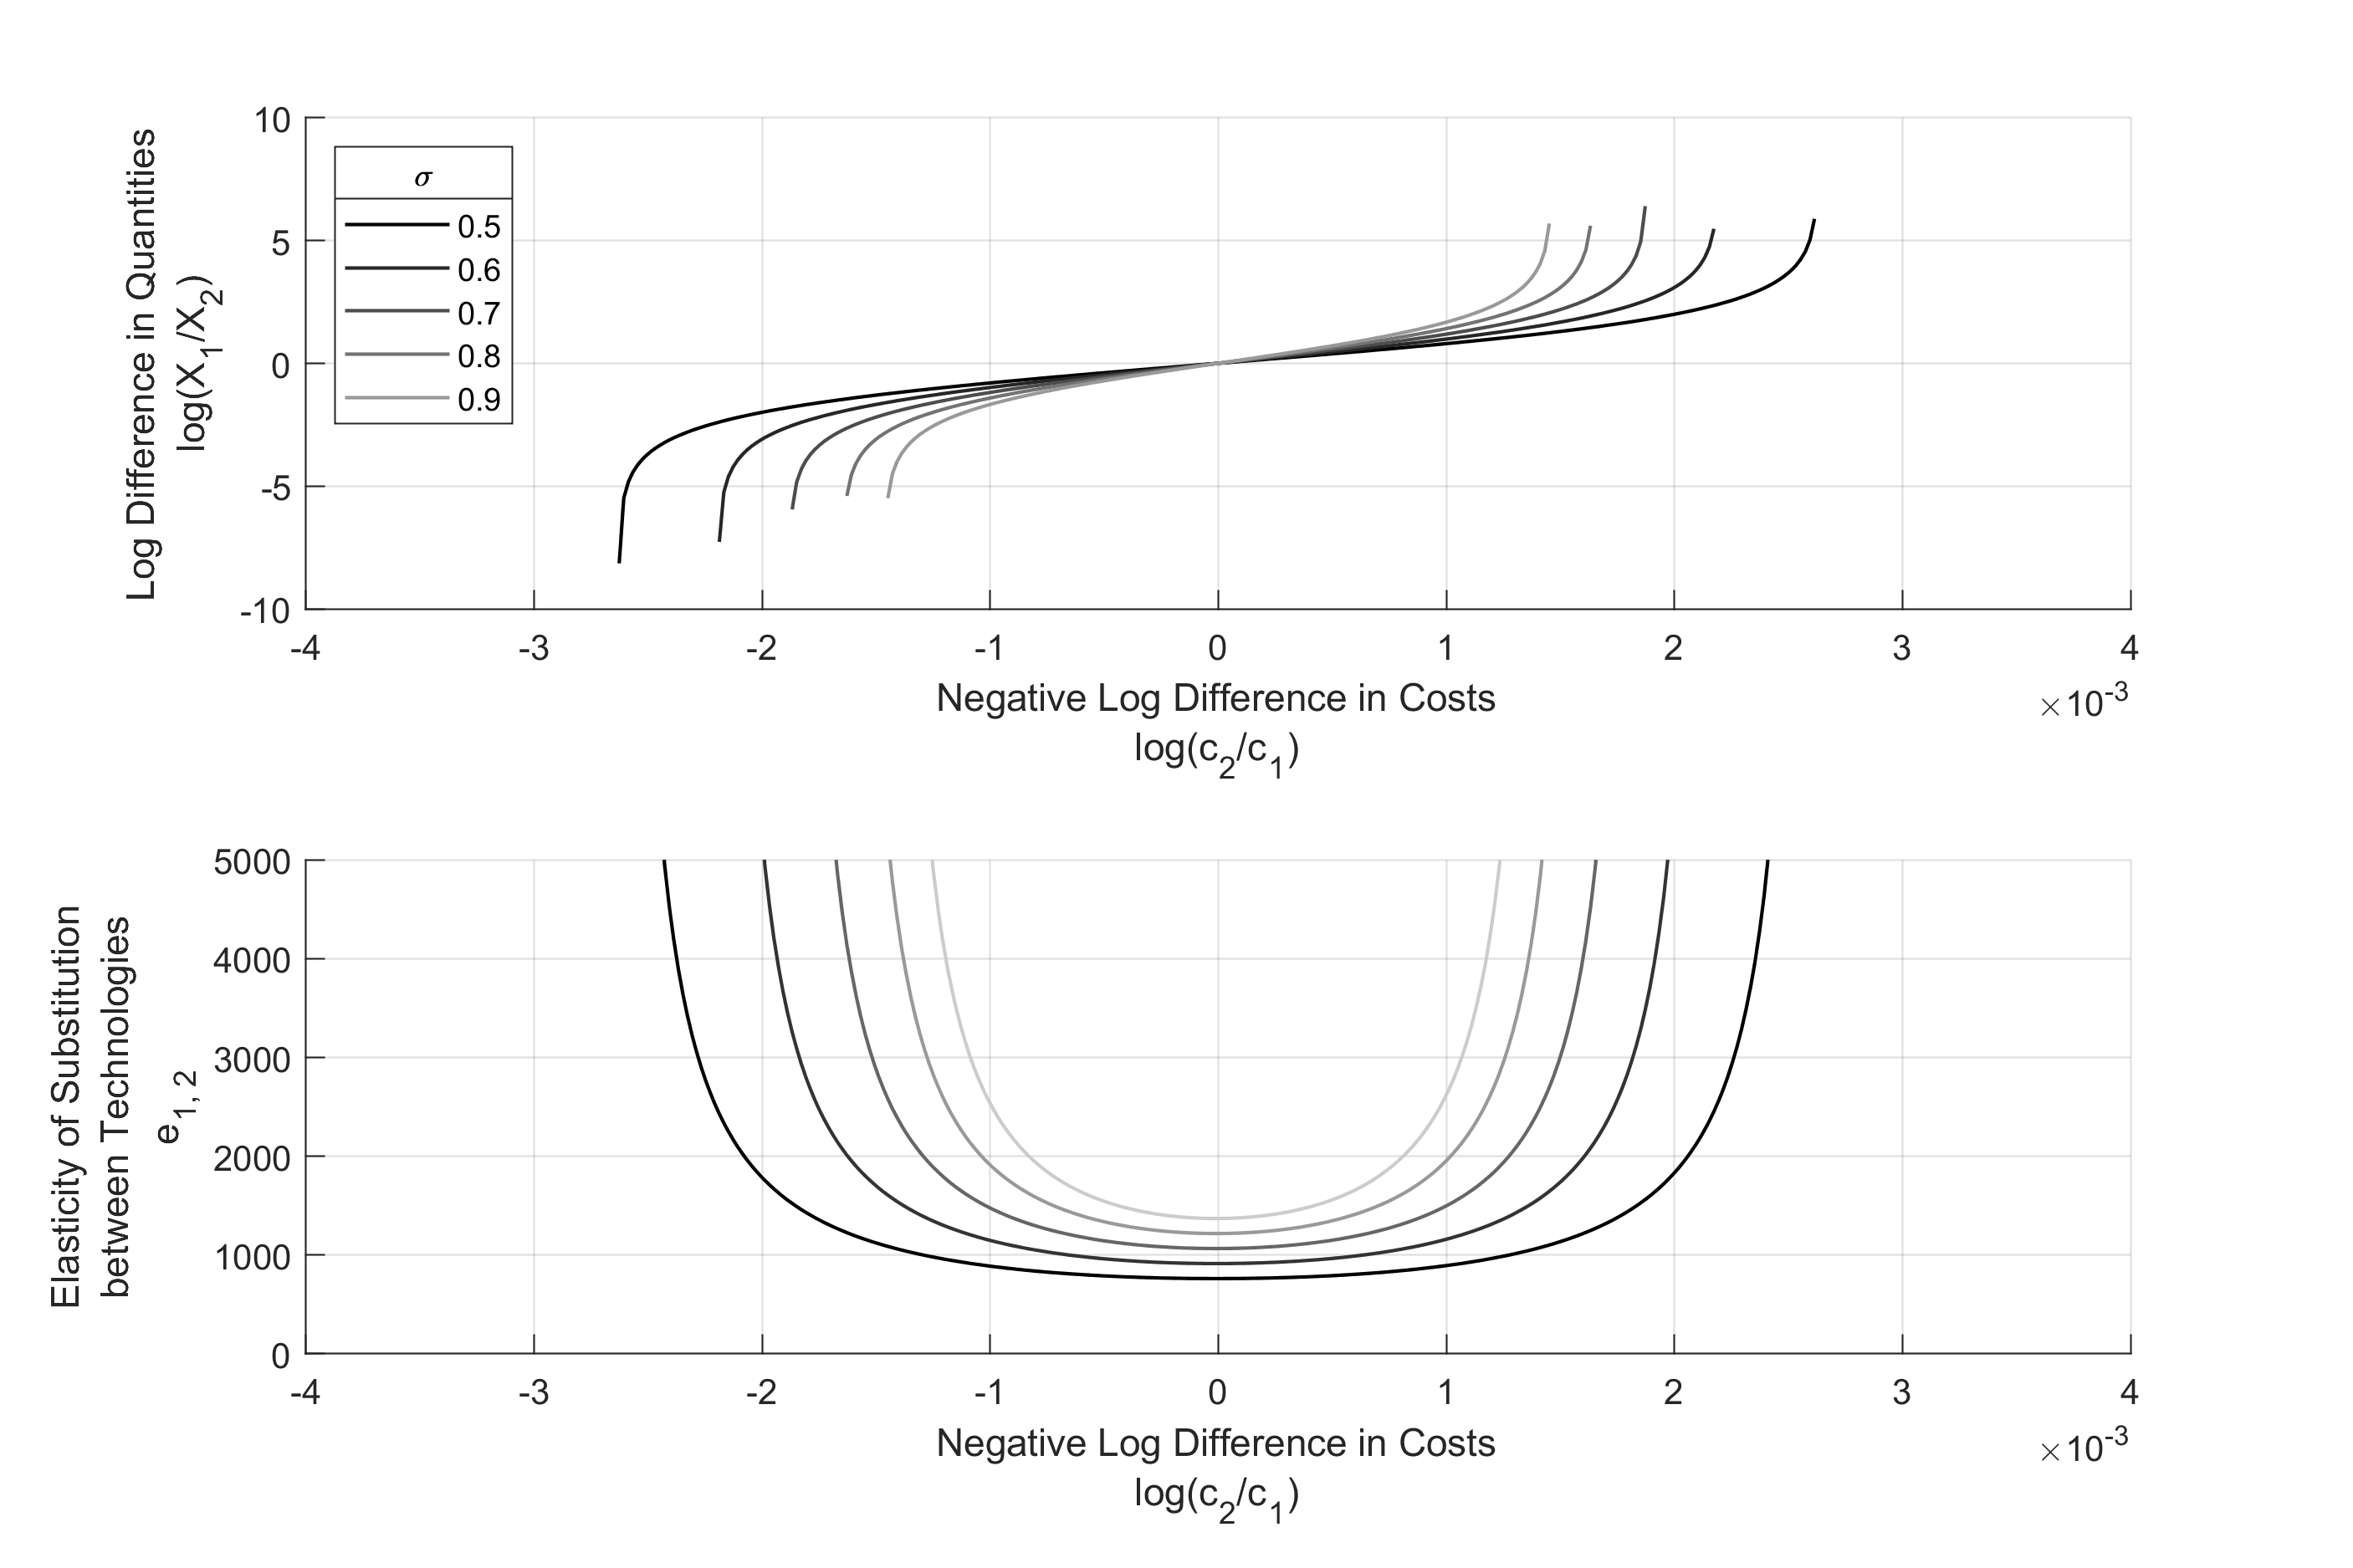
\includegraphics[width=1\linewidth]{../figures/fig_elasticity_range} \\
			\multicolumn{1}{@{\hspace{0.2in}}p{5.9in}@{}}{ \textit{Note: } The y-axis of the first plot is equivalent to $\log(X_1/X_2)$ and the x-axis of both plots is equivalent to  $\log(c_2/c_1)$. Technology 1 and 2 represent two arbitrary technologies that are practically non-intermittent. The legend in the upper subplot also applies to the lower subplot. These results were obtained using the following parameters: $\alpha_t = 0.5$, $\alpha_s = 0.5$, $\xi_1 = (0.95, \, 1)$, $\xi_2 = (1, \, 0.95)$, $c_1 = 100$, $c_2 = 100$. In order to generate these numerical results, we first found the optimal quantities of $\mathbf{X}$ over a range of prices $c_1^* \in (0.5\, c_1, 1.5 \,c_1)$. Then, we obtained estimates of the elasticity of substitution by numerically differentiating $\ln(X_1/X_2)$ with respect to $-\ln(c_1, c_2)$. That is, the elasticity of substitution  between technology 1 and 2 is given by the slope of the upper subplot, and it is graphed in the lower subplot. Finally, we repeat this procedure for various values of $\sigma$. }     \\  
		\end{tabular}
	\end{figure}
	\clearpage
	
	
	\begin{figure}[h!]
		\captionsetup{format=centerproper}
		\caption{The VES Approximation of the Elasticity of Substitution \\ between Highly Intermittent Solar and Coal} 
		\label{fig:ves_int}
		\footnotesize
		\vspace{-1em}
		\begin{tabular}{@{\extracolsep{0em}}c}
			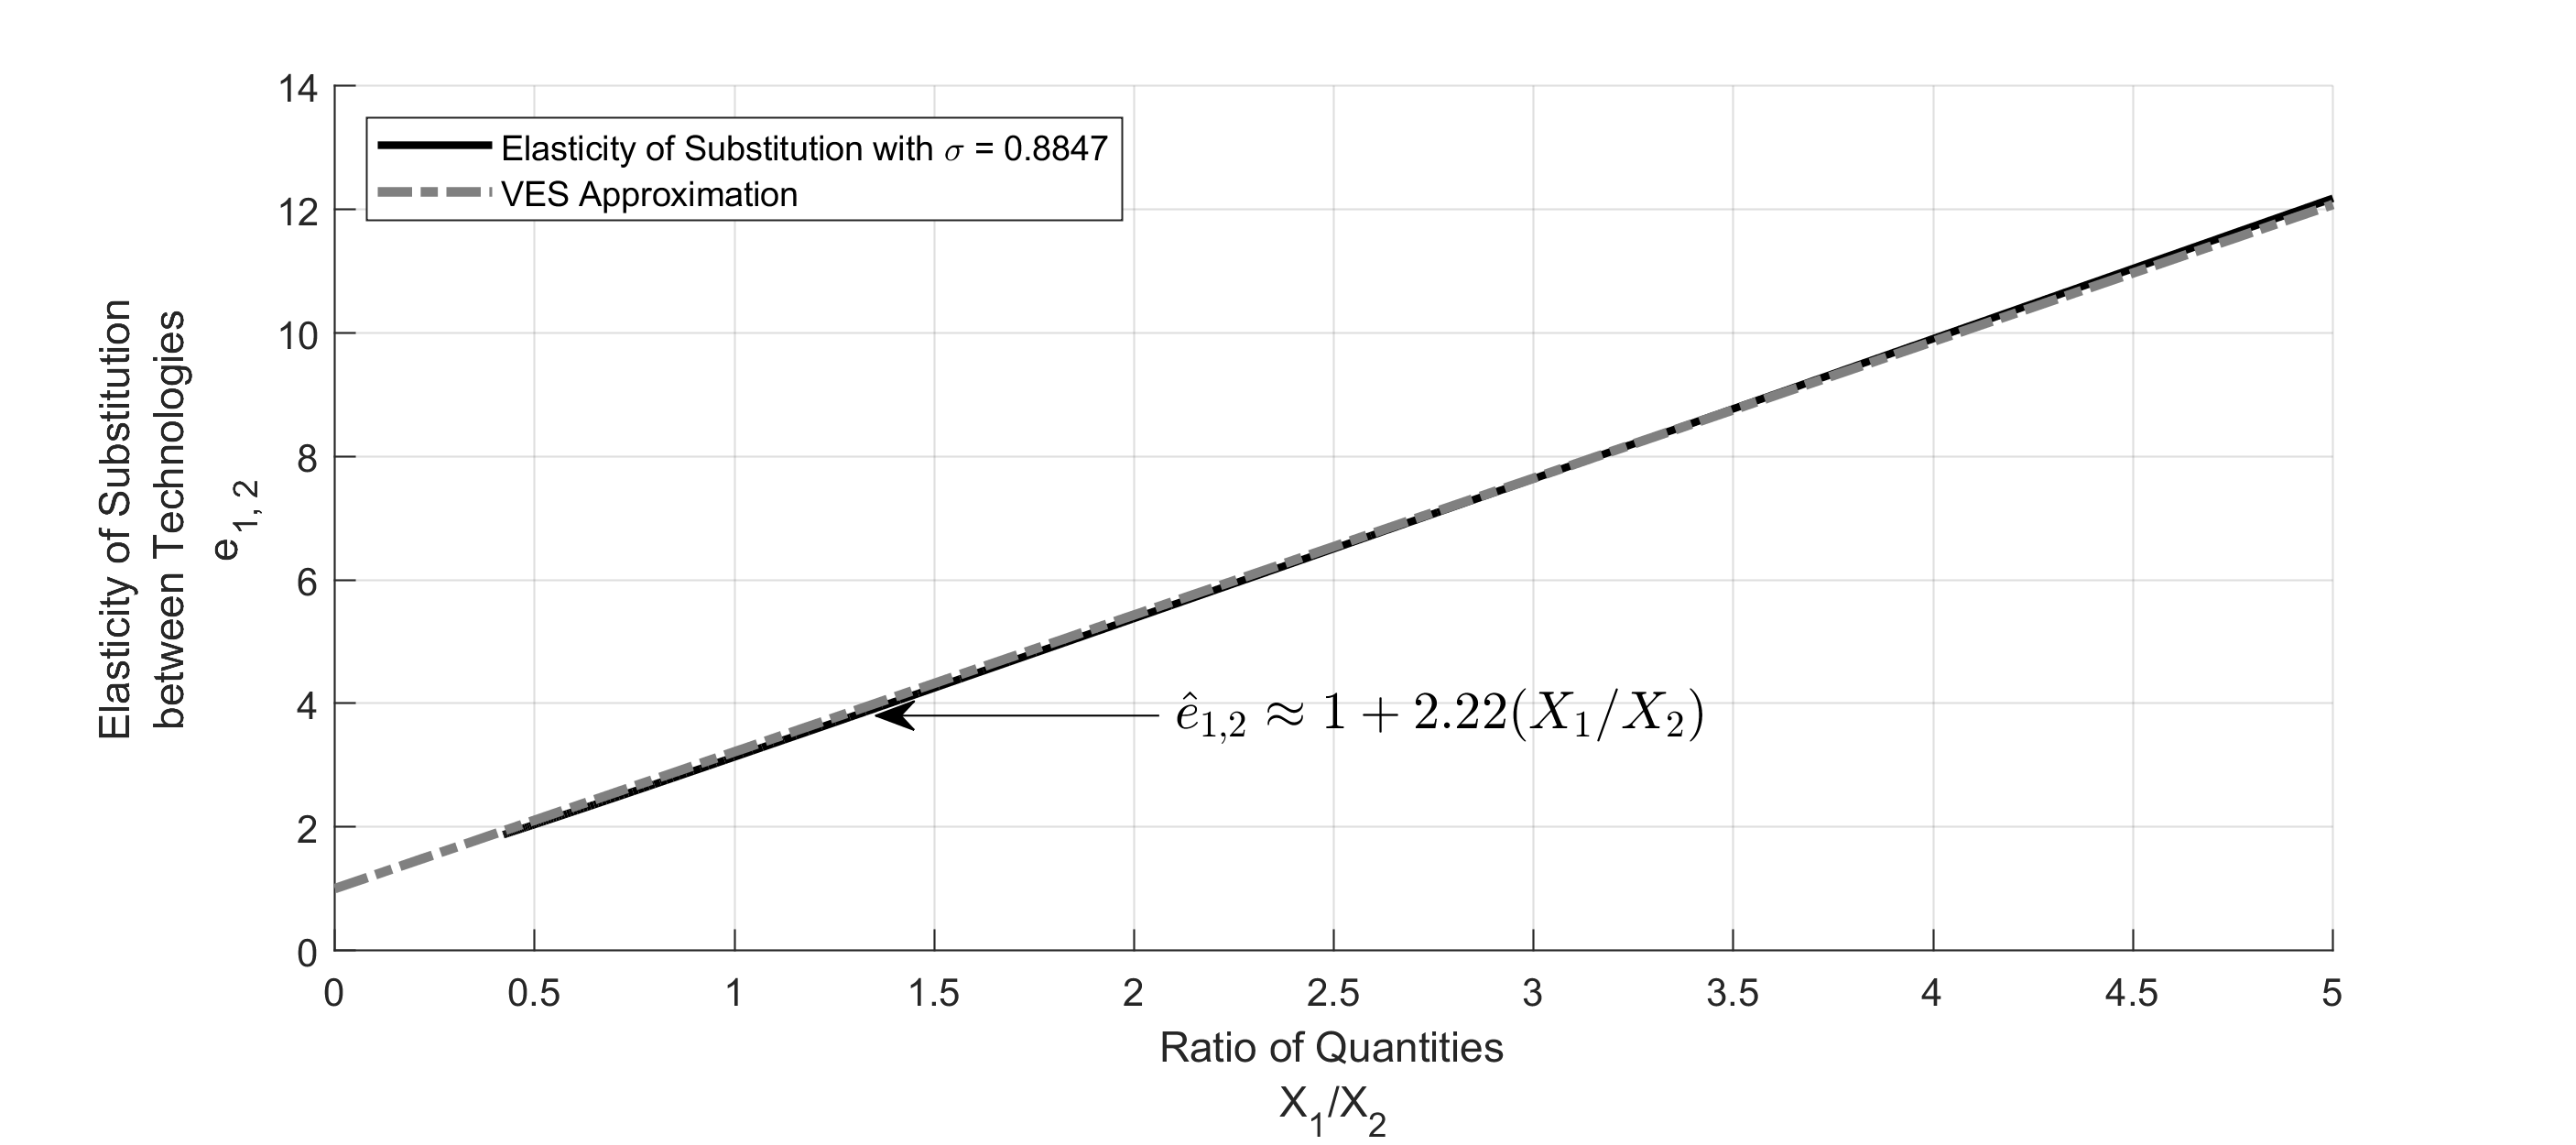
\includegraphics[width=1\linewidth]{../figures/fig_ves_approx_int} \\
			\multicolumn{1}{@{\hspace{0.2in}}p{5.9in}@{}}{ \textit{Note: } Technology 1 is coal and technology 2 is solar. The purple, dash-dots line represents a linear approximation of $e_{1,2}$ for $\sigma = 0.8847$ with a fixed intercept of 1. These results were obtained using the following parameters: $\alpha_t = 0.6$, $\alpha_s = 0.4$, $\xi_1 = (1, \, 1)$, $\xi_2 = (1, \, 0.01)$, $c_1 = 104.3$, $c_2 = 60$. Furthermore, we set the parameter for the intertemporal elasticity of substitution for electricity consumption equal to our estimate $\hat{\sigma} = 0.8847$. In order to generate these numerical results, we first found the optimal quantities of $\mathbf{X}$ over a range of prices $c_1^* \in (c_1, 2 \,c_1)$. Then, we obtained estimates of the elasticity of substitution by numerically differentiating $\ln(X_1/X_2)$ with respect to $-\ln(c_1, c_2)$.  }     \\  
		\end{tabular}
	\end{figure}
	\clearpage
	

	
\end{document}





